%%%  Ukázkový text a dokumentace stylu pro text závěrečné (bakalářské a
%%%  diplomové) práce na KI PřF UP v Olomouci
%%%  Copyright (C) 2012 Martin Rotter, <rotter.martinos@gmail.com>
%%%  Copyright (C) 2014 Jan Outrata, <jan.outrata@upol.cz>


%%  Pro získání PDF souboru dokumentu je třeba tento zdrojový text v
%%  LaTeXu přeložit (dvakrát) programem pdfLaTeX.

%%  V případě použití programu BibLaTeX pro tvorbu seznamu literatury
%%  je poté ještě třeba spustit program Biber s parametrem jméno
%%  souboru zdrojového textu bez přípony a následně opět (dvakrát)
%%  přeložit zdrojový text programem pdfLaTeX.

%%  Postup získání Postscriptového souboru je popsán v dokumentaci.


%%  Třída dokumentu implementující styl pro závěrečnou práci. Vybrané
%%  nepovinné parametry (ostatní v dokumentaci):

%%  'master' pro sazbu diplomové práce, jinak se sází bakalářská práce

%%  'field=kód' pro Váš studijní obor, kódy pro diplomovou práci 'uvt'
%%  pro Učitelství výpočetní techniky pro střední školy a 'binf' pro
%%  Bioinformatiku, jinak je výchozí Informatika, a pro bakalářskou
%%  práci 'ainfk' pro Aplikovanou informatiku v kombinované formě,
%%  'inf' pro Informatiku, 'infv' pro Informatiku pro vzdělávání a
%%  'binf' pro Bioinfomatiku, jinak je výchozí Aplikovaná informatika
%%  v prezenční formě

%%  'printversion' pro sazbu verze pro tisk (nebarevné logo a odkazy,
%%  odkazy s uvedením adresy za odkazem, ne odkazy do rejstříku),
%%  jinak verze pro prohlížeč

%%  'biblatex' pro zapnutí podpory pro sazbu bibliografie pomocí
%%  BibLaTeXu, jinak je výchozí sazba v prostředí thebibliography

%%  'language=jazyk' pro jazyk práce, jazyky english pro anglický,
%%  slovak pro slovenský, jinak je výchozí czech pro český

%%  'font=sans' pro bezpatkový font (Iwona Light), jinak výchozí
%%  patkový (Latin Modern)

\documentclass[
  master,
  field=inf,
  %printversion,
  biblatex=true,
  language=czech,
  theorems=false,
  sourcecodes=false,
  glossaries=false,
  index=false,
]{kidiplom}

%% Informace pro úvodní strany. V jazyku práce (pokud není v komentáři
%% uvedeno česky) a anglicky. Uveďte všechny, u kterých není v
%% komentáři uvedeno, že jsou volitelné. Při neuvedení se použijí
%% výchozí texty. Text pro jiný než nastavený jazyk práce (nepovinným
%% parametrem language makra \documentclass, výchozí český) se zadává
%% použitím makra s uvedením jazyka jako nepovinného parametru.

%% Název práce, česky a anglicky. Měl by se vysázet na jeden řádek.
\title{Aplikace fuzzy a pravděpodobnostních automatů}
\title[english]{Applications of fuzzy and probabilistic automata}

%% Volitelný podnázev práce, česky a anglicky. Měl by se vysázet na
%% jeden řádek. Výchozí je prázdný.
%\subtitle{}
%\subtitle[english]{}

%% Jméno autora práce. Makro nemá nepovinný parametr pro uvedení
%% jazyka.
\author{Bc.~Martin~Jašek}

%% Jméno vedoucího práce (včetně titulů). Makro nemá nepovinný
%% parametr pro uvedení jazyka.
\supervisor{doc.~RNDr.~Michal Krupka,~Ph.D.}

%% Volitelný rok odevzdání práce. Výchozí je aktuální (kalendářní)
%% rok. Makro nemá nepovinný parametr pro uvedení jazyka.
%\yearofsubmit{\the\year}

%% Anotace práce, včetně anglické (obvykle překlad z jazyka
%% práce). Jeden odstavec!
\annotation{Fuzzy a pravděpodobnostní automaty jsou poměrně moderní výpočetní modely. Tato práce se zabývá jejich uplatněním v praxi. Práce prezentuje značné množství oblastí, kde nacházejí tyto modely uplatnění, a to včetně konkrétních příkladů jejich aplikací. Součástí práce je software, který některé aplikace implementuje.}

\annotation[english]{Fuzzy and probabilistic automata are quite modern computational models. This thesis is about their practical applications. Thesis presents considerable amount of domains, where theese models find usage, so with the particular examples of their applications. This thesis also includes software, which some of such applications implements.}

%% Klíčová slova práce, včetně anglických. Oddělená (obvykle) středníkem.
\keywords{automaty; fuzzy množiny; pravděpodobnostní počet; aplikace}
\keywords[english]{automata; fuzzy sets; probability; applications}

%% Volitelná specifikace příloh textu práce, i anglicky. Výchozí je '1
%% CD/DVD'.
%\supplements{jedno kulaté placaté CD/DVD s malou kulatou dírou uprostřed}
%\supplements[english]{one round flat CD/DVD with a small round hole in the middle}

%% Volitelné poděkování. Stručné! Výchozí je prázdné. Makro nemá
%% nepovinný parametr pro uvedení jazyka.
\thanks{Chtěl bych poděkovat vedoucímu práce, doc.~RNDr.~Michalovi Krupkovi,~Ph.D., za velmi cenné a přínosné rady. Dále bych chtěl poděkovat všem mým blízkým, kteří mi po dobu vypracovávání této práce byli oporou.}

%% Cesta k souboru s bibliografií pro její sazbu pomocí BibLaTeXu
%% (zvolenou nepovinným parametrem biblatex makra
%% \documentclass). Použijte pouze při této sazbě, ne při (výchozí)
%% sazbě v prostředí thebibliography.
\bibliography{resources.bib}

%% Další dodatečné styly (balíky) potřebné pro sazbu vlastního textu
%% práce.
%%%%%%%%%%%%%%%%%%%%%%%%%%%%%%%%%%%%%%%%%%%%%%%%%%%%%%%%%%%%%%%%%%%%%
%% různé matematické package
\usepackage{amsthm}
\usepackage{amsmath}
\usepackage{amsfonts}
\usepackage{amssymb}
\usepackage{mathrsfs}
\usepackage{mathtools}

%% číslovaný cases
\usepackage[subnum]{cases}

%% colspan a rowspan v tabulkách
\usepackage{multirow}


%% subfigures, https://en.wikibooks.org/wiki/LaTeX/Floats,_Figures_and_Captions#Subfloats
\usepackage{subcaption}

%% zobrazování labelů, http://tex.stackexchange.com/a/361157
%\usepackage{showlabels}

%% číslování řádků, https://texblog.org/2012/02/08/adding-line-numbers-to-documents/
%\usepackage{lineno}

%% chorvatská jména autorů, https://tex.stackexchange.com/questions/14872/croatian-serbian-letters-in-cv-problem
\usepackage[T1]{fontenc}

%% zalamování URL, https://tex.stackexchange.com/questions/298851/linebreak-in-long-url-breakurl-wont-break-it/298856
%%\usepackage[anythingbreaks]{breakurl}

%% česká sazba bibtexu, https://tex.stackexchange.com/questions/194830/biber-locale-does-not-match-system-language-nor-biblatex-language
%\usepackage[czech]{babel}

%% https://tex.stackexchange.com/questions/4465/put-a-slash-through-a-word?rq=1
%% \usepackage{cancel}

%% \verb , https://tex.stackexchange.com/questions/2790/when-should-one-use-verb-and-when-texttt
%\usepackage{verbatim}

%Definice, věta, důkaz!
%\newtheorem{definition}{Definice}
%\newtheorem{theorem}{Věta}
\newtheorem*{notation*}{Značení} %\TODO{nahrazeno 'notation'}
\newtheorem{notation}{Značení}
\newtheorem{note}{Poznámka}
%\newtheorem{example}{Příklad}


\numberwithin{definition}{section}
\numberwithin{theorem}{section}
%\numberwithin{notation}{section}
\numberwithin{note}{section}
\numberwithin{example}{section}


%Ostatní makra
\newcommand{\TODO}[1]{ } 	%\textit{\small(zde bude doplněno: #1)}} 
\newcommand{\RLY}{?? }

\newcommand{\lattL}{\mathbb{L}}
\newcommand{\fsubsets}[1]{\mathcal{F}(#1)}

\newcommand{\term}[1]{\textit{#1}}
\newcommand{\str}[1]{{\textit{#1}}}
\newcommand{\regex}[1]{{\ttfamily#1}}
\newcommand{\ifthen}{\textsc{If--Then} }

\newcommand{\impl}[2]{{\ttfamily#1/}{\ttfamily test/data/}{\ttfamily#2}}

%%%%%%%%%%%%%%%%%%%%%%%%%%%%%%%%%%%%%%%%%%%%%%%%%%%%%%%%%%%%%%%%%%%%%

\begin{document}
%% Sazba úvodních stran -- titulní, s bibliografickými údaji, s
%% anotací a klíčovými slovy, s poděkováním a prohlášením, s obsahem a
%% se seznamy obrázků, tabulek, vět a zdrojových kódů (pokud jejich
%% sazba není vypnutá).
\maketitle

%% -------------------------------------------------------------------

% \documentclass[a4paper,10pt]{article}
% \usepackage[utf8x]{inputenc}
% \usepackage[czech]{babel}
% 
% \usepackage{amsthm}
\usepackage{amsmath}
\usepackage{amsfonts}
\usepackage{mathtools}

%% číslovaný cases
\usepackage[subnum]{cases}

%% colspan a rowspan v tabulkách
\usepackage{multirow}

%%  http://tex.stackexchange.com/a/361157
\usepackage{showlabels}

%% subfigures, https://en.wikibooks.org/wiki/LaTeX/Floats,_Figures_and_Captions#Subfloats
\usepackage{subcaption}

%% číslování řádků, https://texblog.org/2012/02/08/adding-line-numbers-to-documents/
\usepackage{lineno}

%Definice, věta, důkaz!
\newtheorem{definition}{Definice}
\newtheorem{theorem}{Věta}
\newtheorem*{notation*}{Značení}
\newtheorem{note}{Poznámka}
\newtheorem{example}{Příklad}


\numberwithin{definition}{section}
\numberwithin{theorem}{section}
%\numberwithin{notation}{section}
\numberwithin{note}{section}
\numberwithin{example}{section}


%Ostatní makra
\newcommand{\TODO}[1]{ \textit{\small(zde bude doplněno: #1)} }	
\newcommand{\RLY}{?? }

\newcommand{\lattL}{\mathbb{L}}
\newcommand{\fsubsets}[1]{\mathcal{F}(#1)}

\newcommand{\term}[1]{\textit{#1}}
\newcommand{\str}[1]{{\ttfamily#1}}
\newcommand{\regex}[1]{{\ttfamily#1}}

\newcommand{\impl}[2]{{\ttfamily#1/}{\ttfamily test/data/}{\ttfamily#2}}

% Speciální nastavení

% vycentrované floating objekty
% http://tex.stackexchange.com/questions/2651/should-i-use-center-or-centering-for-figures-and-tables
\makeatletter
\g@addto@macro\@floatboxreset\centering
\makeatother

\linenumbers
\modulolinenumbers[10]

% 
% %opening
% \title{Aplikace fuzzy a pravděpodobnostních automatů}
% \author{Martin Jašek}
% \date{12. září 2016 --- ???}
% 
% \begin{document}
% 
% \maketitle
% \tableofcontents
% \newpage

%%%%%%%%%%%%%%%%%%%%%%%%%%%%%%%%%%%%%%%%%%%%%%%%%%%%%%%%%%%%%%%%%%%%%%%%%%%%%%%
%%%%%%%%%%%%%%%%%%%%%%%%%%%%%%%%%%%%%%%%%%%%%%%%%%%%%%%%%%%%%%%%%%%%%%%%%%%%%%%
%%%%%%%%%%%%%%%%%%%%%%%%%%%%%%%%%%%%%%%%%%%%%%%%%%%%%%%%%%%%%%%%%%%%%%%%%%%%%%%
%%%%%%%%%%%%%%%%%%%%%%%%%%%%%%%%%%%%%%%%%%%%%%%%%%%%%%%%%%%%%%%%%%%%%%%%%%%%%%%
\section{Úvod}
Fuzzy automaty jsou výpočetní modely, které propojují teorii automatů s fuzzy množinami. Obdobně, pravděpodobnostní automaty spojují teorii automatů s pravděpodobnostním počtem.

Teorie automatů, fuzzy množiny i pravděpodobnostní počet jsou v současné době poměrně hluboce prozkoumány. Je proto přirozené, že se současný výzkum zabývá také jejich vzájemným propojováním, tj. fuzzy a pravděpodobnostními automaty. Teoretický výzkum těchto modelů přinesl mnohé výsledky. Otázkou však je, jaké je uplatnění těchto modelů v praxi.

Fuzzy množiny a pravděpodobnostní počet slouží k popisu různých forem neurčitosti, nepřesnosti či nejistoty. To jsou jevy, se kterými se setkáváme v běžném životě prakticky denně. Fuzzy a pravděpodobnostní automaty by tak mohly mít velký potenciál pro uplatnění v praxi. Úkolem této práce je tuto hypotézu ověřit.

V první části této práce jsou uvedeny základní teoretické poznatky studia fuzzy a pravděpodobnosních automatů. Druhá část práce je poté věnována popisu samotných aplikací. Kromě teoretického popisu možností uplatnění tato práce prezentuje reálné ukázky uplatnění a konkrétní příklady. Závěr práce je věnován popisu softwaru, který některé z aplikací přímo implementuje.


%%%%%%%%%%%%%%%%%%%%%%%%%%%%%%%%%%%%%%%%%%%%%%%%%%%%%%%%%%%%%%%%%%%%%%%%%%%%%%%
%%%%%%%%%%%%%%%%%%%%%%%%%%%%%%%%%%%%%%%%%%%%%%%%%%%%%%%%%%%%%%%%%%%%%%%%%%%%%%%
%%%%%%%%%%%%%%%%%%%%%%%%%%%%%%%%%%%%%%%%%%%%%%%%%%%%%%%%%%%%%%%%%%%%%%%%%%%%%%%
%%%%%%%%%%%%%%%%%%%%%%%%%%%%%%%%%%%%%%%%%%%%%%%%%%%%%%%%%%%%%%%%%%%%%%%%%%%%%%%
\section{Úvodní pojmy}
V této kapitole budou popsány základní pojmy, bez kterých nebude možné se studiu fuzzy a pravděpodobnostních automatů věnovat. Bude zde představen koncept fuzzy množin, pravděpodobnostního počtu a základní pojmy z teorie automatů.

%%%%%%%%%%%%%%%%%%%%%%%%%%%%%%%%%%%%%%%%%%%%%%%%%%%%%%%%%%%%%%%%%%%%%%%%%%%%%%%
\subsection{Fuzzy množiny a fuzzy logika}
Pomocí matematiky můžeme formalizovat svět kolem nás. Zatímco matematika je založena na přesnosti, většinu okolního světa lze přesně popsat jen s těží. Při popisu okolního světa pracujeme mnohem častěji s vágními pojmy jako \uv{málo}, \uv{téměř} či \uv{trochu} než s jednoznačným \uv{ano} a \uv{ne}. Například, tvrzení \uv{student učivo umí} lze těžko ohodnotit pravdou či nepravdou, pokud student z testu získal $50\%$ bodů. Naopak, říci, že \uv{student učivo umí z $1/2$} je mnohem přirozenější. V případech jako je tento mohou fuzzy množiny přinést značné zpřehlednění.

Podobně jako například predikátová logika tvoří matematický nástroj pro popis logického uvažování, fuzzy množiny (případně fuzzy logiky od nich odvozené) jsou matematický nástroj pro práci s nepřesnými pojmy\footnote{Slovo \uv{fuzzy} v angličtině znamená \uv{nejasný}, \uv{rozmazaný}, \uv{neostrý}}. Oproti \uv{klasické} množině, která prvek buďto obsahuje nebo neobsahuje, fuzzy množině může prvek nálažet v určitém stupni, který se nachází někde mezi \uv{nenáleží vůbec} a \uv{náleží plně}. Obdobně, pravdivost tvrzení (tedy formule vyjádřené v přirozeném jazyce) ve fuzzy logice nemusí být pouze pravdivé či nepravdivé, ale může nabývat libovolného stupně pravdivosti.

Fuzzy množiny jsou tedy matematickým nástrojem. Následuje jejich formální definice. Definice a související pojmy jsou přejaty z \cite{Bel-FuzRelSys}.

\begin{definition}[Fuzzy množina]
 Mějme libovolnou neprázdnou množinu $U$ (tzv. univerzum). Pak zobrazení $\rho: U \rightarrow [0, 1]$ nazvěme fuzzy množina nad $U$. Pro $x \in U$ říkáme, že prvek $x$ náleží do množiny $\rho$ ve stupni $\rho(x)$.
\end{definition}

\begin{notation*}
 Abychom rozlišili \uv{klasické} (tzv. bivalentní) množiny od fuzzy množin, budou fuzzy množiny v tomto textu obvykle značeny malými řeckými písmeny. Fakt, že fuzzy množina $\rho$ obsahuje prvky $x_1, \dots, x_n \in U$ ve stupních $d_1, \dots, d_n \in [0,1]$ budeme psát $\rho = \{ x_1 / d_1, \dots x_n / d_n \}$. 
\end{notation*}

V této práci se dopouštíme význameného zjednodušení. Množina stupňů pravdivosti, kterou zde uvažujeme jako interval $[0, 1]$, může být ve skutečnosti mnohem obecnější. Takové zobecnění by však vyžadovalo výrazně hlubší popis jejich vlastnostní, který je u intervalu $[0, 1]$ intuitivní. Navíc, použití intervalu $[0, 1]$ je pro člověka přirozené, $0$ přirozeně odpovídá \uv{nulové pravdivosti} a $1$ \uv{plné pravdivosti}. V neposlední řadě, použití intervalu $[0, 1]$ je výhodné také kvůli snadné implementaci na počítači.


Nyní se podíváme na základní operace nad fuzzy množinami.

\begin{definition}[Operace nad fuzzy množinami]
 Mějme dvě fuzzy množiny $\pi$ a $\rho$ nad univerzem $U$. Pak definujme jejich průnik, sjednocení a doplňěk (komplement) jako fuzzy množiny $\pi \cap \rho$, $\pi \cup \rho$ a $\neg \pi$ nad téže univerzem, které pro všechna $x \in U$ splňují:
 \begin{align*}
  (\pi \cap \rho)(x) 	\; &= \; \pi(x) \wedge \rho(x) \\
  (\pi \cup \rho)(x) 	\; &= \; \pi(x) \vee \rho(x) \\
  (\neg \pi)(x) 	\; &= \; 1 - \pi(x) \\
 \end{align*}
\end{definition}

\begin{definition}[Relace mezi fuzzy množinami]
 Mějme dvě fuzzy množiny $\pi$ a $\rho$ nad univerzem $U$. Pak definujme jejich rovnost a inkluzi (relaci \uv{býti podmnožinou}) jako relace $=,\subseteq: (U \rightarrow [0,1]) \times (U \rightarrow [0,1])$:
 \begin{align*}
  \pi = \rho 		&\text{ právě tehdy když } \pi(x) = \rho(x) 	\text{ pro každé $x \in U$}	\\
  \pi \subseteq \rho 	&\text{ právě tehdy když } \pi(x) \leq \rho(x) 	\text{ pro každé $x \in U$}	\\	
 \end{align*}
\end{definition}

Připomeňme, že operátory $\wedge$ a $\vee$ na reálném intervalu $[0, 1]$ jsou definovány jako $\min$ a $\max$. Operátor $\le$ značí přirozené uspořádání čísel a $=$ jejich rovnost.

Kromě operací s fuzzy množinami ještě budeme pracovat s operacemi t-norma a t-konorma, což jsou binární operace na množině $[0,1]$.
\begin{definition}[T-norma a t-konorma]
 Binární operace $\otimes$ (t-norma) na množině $[0,1]$ je asociativní, komutativní, monotonní operátor s neutrálním prvkem $1$.
 Binární operace $\oplus$  (t-konorma) na množině $[0,1]$ je asociativní, komutativní, monotonní operátor s neutrálním prvkem $0$.
\end{definition}

Operace t-norma a t-konorma si lze představit jako zobecnění disjunkce a konjunkce. Je proto vhodné, aby t-norma a t-konorma splňovaly zobecněný De~Morganův zákon, tj. aby pro všechna $a, b \in [0,1]$ platila následující rovnost:
$$
  a \oplus b = 1 - ((1 - a) \otimes (1 - b))
$$
popř. ekvivalentně:
$$
  a \otimes b = 1 - ((1 - a) \oplus (1 - b))
$$

V tabulce \ref{tbl:Norms} jsou uvedeny nejpoužívanější tři t-normy a jim odpovídající t-konormy, tak, aby splňovaly zobecněný De~Morganův zákon.
\begin{table}
 \centering
 \begin{tabular}{|l|l||l|l|}
  \hline
  \multicolumn{2}{|c||}{t-norma}			& \multicolumn{2}{|c|}{t-konorma}			\\\hline 
  název	 		& $a \otimes b$		& název				& $a \oplus b$		\\\hline \hline
  Gödelova 		& $\min(a, b)$ 		& maximální 			& $\max(a, b)$		\\
  (minimální) 		&			&				&			\\\hline
  Produktová 		& $a b$ 		& probabilistický  		& $a + b - a b$		\\
			&			& součet			&			\\\hline
  \L{}ukasiewiczova 	& $\max(0, a + b - 1)$ 	& ohraničený 			& $\min(a + b, 1)$	\\
			&			& součet			&			\\\hline
 \end{tabular}

 \caption[Tři nejpoužívajší t-normy]{Tři nejpoužívajší t-normy a jim odpovídající t-konormy tak, aby splňovaly zobecněný De~Morganův zákon}
 \label{tbl:Norms}
\end{table}

Množinu všech fuzzy množin nad univerzem $U$ (tedy protějšek potenční množiny u \uv{klasických} množin) budeme značit $\fsubsets{U}$. Posledním z důležitých pojmů je fuzzy relace.

\begin{definition}[Fuzzy relace]
 Jako fuzzy relaci na fuzzy množinách $U_1, \dots, U_n$ nazýváme fuzzy množinu nad $U_1 \times \dots \times U_n$ (tj. nad kartézským součinem těchto množin).
\end{definition}

\begin{example}[Fuzzy množiny a fuzzy relace]
  Příkladem fuzzy množiny může být fuzzy množina reálných čísel, která jsou blízko nule. Taková fuzzy množina bude mít univerzum $U = \mathbb{R}$ a předpis například $\zeta(x) = 2^{-|x|}$, tj. $\zeta(x) = \{ x/d | x \in \mathbb{R}, d = 2^{-|x|} \}$. Pak platí $\zeta(0) = 1$ (tj. číslo $0$ je blízko nule v jednotkovém stupni), $\zeta(1) = 1/2$ (tj. pravdivost tvrzení \uv{číslo $1$ je blízko nule} je $0{,}5$), $\zeta(2) = 1/4$ a podob.
  
  Příklad fuzzy relace může být podobnost čísel. Tedy fuzzy relace popsiující vztah \uv{čísla $x$ a $y$ jsou si podobná ve stupni $\sigma(x, y)$}. Jedná se tedy o fuzzy relaci na $\mathbb{R} \times \mathbb{R}$ a dána může být například předpisem: $\sigma(x, y) = 2^{-|x-y|}$. Přirozeně, pak platí například $\sigma(1, 1) = 1$, $\sigma(1, 2) = 1/2$, $\sigma(1, 3) = 1/4$ a podob.
\end{example}

%%%%%%%%%%%%%%%%%%%%%%%%%%%%%%%%%%%%%%%%%%%%%%%%%%%%%%%%%%%%%%%%%%%%%%%%%%%%%%%
\subsection{Pravděpodobnostní počet}
Pravděpodobnost je další způsob popisu neurčitosti. Pozorujeme-li nějaký jev, pak pravděpodobnost vyjadřuje, jak moc je jisté, že tento jev nastane i v budoucnu. 

Z pohledu aplikací pravděpodobnostních automatů pro nás bude pravděpodobnost -- podobně, jako stupeň pravdivosti -- číslo z reálného intervalu $[0, 1]$ s některými dalšími vlastnostmi. Definice a vlastnosti pravděpodobností zde budou uvedeny ve zjednodušené podobě a jsou převzaty z \cite{Joh-ProbStaComSci}. 

\begin{definition}[Prostor jevů, jev]
  Označme neprázdnou množinu $\Omega$ jako prostor jevů, její prvky jako elementární jevy a její podmnožiny jako jevy.  
\end{definition}

\begin{definition}[Pravděpodobnost elementárních jevů]
 Pravděpodobnost (resp. pravděpodobnostní míra) elementárního jevu je zobrazení $P: \Omega \rightarrow [0,1]$, (tj. zobrazení, které každému elementárnímu jevu $\omega \in \Omega$ přiřazuje jeho pravděpodobnost $P(\omega)$) takové, že $\sum_{\omega \in \Omega} P(\omega) = 1$.
\end{definition}

\begin{definition}[Pravděpodobnostní míra]
 Mějme prostor jevů $\Omega$ a pravděpodobnost $P$ elementárních jevů z tohoto prostoru. Pak jako pravděpodobnost (pravděpodobnostní míra) jevu $A \subset \Omega$ nazýváme zobrazení $P: 2^\Omega \rightarrow [0,1]$ dané následujícím předpisem:
  $$
    P(A) = \sum_{\omega \in A} P(\omega)
  $$
\end{definition}

Libovolná pravděpodobnostní míra $P$ pro každý prostor jevů $\Omega$ a libovolné jevy $A, B \subseteq \Omega$ dále splňuje následující vlastnosti:
\begin{enumerate}
 \item $P(\emptyset) = 0$ (tzv. nemožný jev)
 \item $P(\Omega) = 1$ (tzv. jistý jev)
 \item $P(\overline{A}) = 1 - P(A)$
 \item $P(A \cap B) = P(A) P(B)$
 \item $P(A \cup B) \leq P(A) + P(B)$
 \item $P(A \cup B) = P(A) + P(B) - P(A \cap B)$
\end{enumerate}

Dalším důležitým pojmem je podmíněná pravděpodobnost. Zjednodušeně řečeno, podmíněná pravděpodobnost nám říká, s jakou pravděpodobností nastal jev $A$ jestliže víme, že nastal jev $B$.

\begin{definition}[Podmíněná pravděpodobnost]
 Mějme pravděpodobností prostor $\Omega$ a dva jevy $A, B \subseteq \Omega$ z tohoto prostoru tak, že $P(B) > 0$. Podmíněná pravděpodobnost jevu $A$ za podmínky, že nastal jev $B$, je pravděpodobnost 
 $$
  P(A | B) = \frac{P(A \cap B)}{P(B)}
 $$
\end{definition}

\begin{example}[Pravděpodobnost]
 Uvažujme příklad s klasickou šestistěnnou hrací kostkou. Prostor jevů je $\Omega = \{ 1,2,3,4,5,6 \}$. Označme $A = \{2, 4, 6\}$ jako jev \uv{padlo sudé číslo} a $B = \{ 5, 6 \}$ jako \uv{padlo číslo větší než $4$}.
 
 Pravděpodobnost jevu $A$ je $\frac{1}{2}$, pravděpodobnost jevu $B$ je $\frac{1}{3}$ a $P(A | B) = 1 / 2$ (tj. pravděpodobnost, že padlo sudé číslo za předpokladu, že padlo číslo větší než $4$ je $1/2$).
\end{example}


%%%%%%%%%%%%%%%%%%%%%%%%%%%%%%%%%%%%%%%%%%%%%%%%%%%%%%%%%%%%%%%%%%%%%%%%%%%%%%%
\subsection{Fuzzy vs. pravděpodobnostní přístup} \label{subsec:FuzzyVsProb}
V předchozích dvou podkapitolách byly zavedeny základní pojmy z oblasti fuzzy množin a pravděpodobnostního počtu. Je vidět, že jak stupeň pravdivosti, tak pravděpodobnostní míra, jsou obě reálná čísla z intervalu $[0, 1]$. Oba tyto pojmy totiž popisují určitou formu neurčitosti, avšak každá jinou. 

Popisujeme-li nějaký jev, pak stupeň pravdivosti udává, jak moc jev odpovídá jeho popisu. Například tvrzení \uv{osoba $X$ je vysoká} může být pravdivé ve stupni $1$, pokud je osoba vysoká $180$ centimetrů a víc a ve stupni $0{,}5$, pokud osoba měří $160$ centimetrů. Popisujeme tedy skutečnost, která je nám známá, avšak při jejím popisu používáme vágní pojem (\uv{vysoká}). Ohodnocení stupňem pravdivosti tak záleží významu tohoto pojmu.

Naopak, tvrzení \uv{zítra mi ujede autobus} je popsáno přesně (nepoužívá žádné vágní pojmy), avšak nejistota je zde skryta v pozorovaném jevu. Zda-li tento jev nastane (a tvrzení je tudíž pravdivé) nebo nenastane nám není známo. Můžeme se však bavit o pravděpodobnosti, s jakou nastane.

Matoucí může být tvrzení \uv{uživatel píše slovo $X$}. Na jednu stranu může být chápáno ve smyslu pravděpodobnosti. Tedy, že na základě určitých pozorování predikujeme s jakou pravděpodobností slovo, které uživatel píše, je slovem $X$. Na druhou stranu toto tvrzení může být chápáno tak, že víme, (se stoprocentní jistotou) jaké slovo uživatel píše, a pak můžeme studovat stupeň pravivosti, v jakém je psané slovo slovem $X$.

Poněkud jinou situací je tvrzení \uv{zítra bude pěkné počasí}. Toto tvrzení totiž obsahuje jak vágní pojem \uv{pěkné}, tak nejistotu (nevíme, jaké bude počasí). Využívá tedy obou přístupů současně.

Při návrhu systému pracujícího s neurčitostí je tedy nutné se vždy zamyslet, jestli jeho neurčitost tkví spíše v nepřesném označení nebo naopak v nepřesné znalosti popisované situace.

\begin{note}
 Existují snahy fuzzy a pravděpodobnostní přístup sjednotit. Takovýmto \uv{univerzálním stupňům neurčitosti} se obvykle říká \uv{váhy}. Systém pracující s vahami však nemá oporu v logickém popisu okolního světa a tak není vhodné jej používat v reálných aplikacích. Sloužit může jen jako teoretický model.
\end{note}


%%%%%%%%%%%%%%%%%%%%%%%%%%%%%%%%%%%%%%%%%%%%%%%%%%%%%%%%%%%%%%%%%%%%%%%%%%%%%%%
\subsection{Popis v přirozeném jazyce}
Vzhledem k tomu, že účelem této práce je studovat uplatění fuzzy a pravděpodobnostních automatů v praxi, je nutné seznámit se s nástroji pro propojení matematického světa (tj. fuzzy množin a pravděpodobnostního počtu) a popisu v přirozeném jazyce.

Pravděpodobnostní počet k tomuto účelu používá slovní označení jevů. Je poměrně přirozené říkat \uv{Pravděpodobnost jevu $e$ je $p$.} nebo \uv{Jev $e$ jistý}.

Pro popis stupňů pravdivosti by bylo možné používat obdobný přístup, tj. říkat \uv{Tvrzení $t$ je pravdivé ve stupni $d$.}. Taková formulace však zní poněkud kostrbatě. Mnohem elegantněji lze podobná tvrzení vyjádřit pomocí tzv. lingvistikých proměnných \cite{Zad-ConLingVarAppApprRea}. Každá lingvistická proměnná $\alpha$ je tvořena univerzem $U$ hodnot a množinou lingvistických štítků $T$. Pro každý štítek $X \in T$ pak $\alpha$ definuje jeho \uv{význam} (významovou funkci) jako fuzzy množinu $M(X)$ nad $U$ (tj. funkci, která hodnotě z univerza přiřadí stupeň pravdivosti). Fakt, že lingvistická proměnná $\alpha$ nabývá \uv{hodnoty} (štítku) $X$ budeme zapisovat $\alpha = X$. Významová funkce štítku $X$ poté určuje stupeň pravdivosti tohoto tvrzení.

\begin{example}[Ligvistické proměnné]
 Mějme lingvistickou proměnnou $\alpha$ s významem \uv{výška osoby}. Univerzem hodnot jsou všechna nezáporná reálná čísla. Lingvistické štítky jsou $X_m$ (\uv{malá}), $X_s$ (\uv{střední}), $X_v$ (\uv{velká}) a $X_{vv}$ (\uv{velmi velká}). Významové funkce jednotlivých štítků jsou vyobrazeny na obrázku \ref{fig:lingVarsMeansChart}.

 Mějme výšku $h$ osoby. Namísto \uv{Platnost tvrzení \uv{výška $h$ osoby je střední} je ve stupni $M(X_s)(h)$} můžeme říkat \uv{výška $h$ osoby je střední}. Symbolicky zapsáno: $\alpha = X_s$.
\end{example}

\begin{figure}
 \centering
 \includegraphics{mpimg-charts0}
 
 \caption[Graf významových funkcí štítků]{Graf významových funkcí štítků $X_m$ (\uv{malá}), $X_s$ (\uv{střední}), $X_v$ (\uv{velká}) a $X_{vv}$ (\uv{velmi velká}) lingvistické porměnné \uv{výška osoby}.} \label{fig:lingVarsMeansChart}
\end{figure}

\begin{note}
 Někdy se můžeme setkat s ligvistickými proměnnými, které mají jen jeden štítek. Například, ligvistická proměnná \uv{závodník se nachází} se štítkem \uv{v cíli}. V takovém případě můžeme psát rovnou \uv{závodník se nachází v cíli}.
\end{note}

Pro popis netriviálních faktů (např. vztahů nebo závislostí) je potřeba pokročilejčí nástroj. Vztahy tak budeme popisovat pomocí tzv. fuzzy \ifthen pravidel\cite{Jan-FouFuzzContPracAppr}. Klasické bivalentní \ifthen pravidlo je výrok ve tvaru:
$$
 \text{Jestliže $x_1$, $\dots$, $x_n$, pak $y$}
$$
kde $x_1, \dots x_n, y$ jsou podvýroky\footnote{Zapíšeme-li \ifthen pravidlo jako formuli, obdržíme Hornovskou klauzuli.}.

\begin{example}[\ifthen pravidla]
 Následující výroky jsou \ifthen pravidla:
 \begin{itemize}
  \item Jestliže je spínač sepnut, pak žárovka svítí
  \item Jestliže je $\text{věk}(p) < 15$, pak $p$ je dítě
  \item Je-li $x \in \mathbb{N}$, $x > 2$, $\nexists y < x: y|x$, pak $x$ je prvočíslo
 \end{itemize}
\end{example}

Fuzzy \ifthen pravidla pak budou vypadat následovně:
$$
 \text{Jestliže $\alpha_1 = x_1$, $\dots$, $\alpha_n = x_n$, pak $\beta = y$}
$$
kde $\alpha_1, \dots \alpha_n, \beta$ jsou lingvistické proměnné a $x_1, \dots, x_n, y$ jsou po řadě jejich štítky.


\begin{example}[Fuzzy \ifthen pravidla]
 Uvažujme systém, u kterého známe tlak (lingvistická proměnná $\alpha_t$) a průtok (lingvistická proměnná $\alpha_p$) a popisujeme úroveň otevření bezpečnostního ventilu (lingvistická proměnná $\alpha_v$). 
 Označme štítky $t_M$ (\uv{tlak je malý}), $t_N$ (\uv{tlak je normální}), $t_V$ (\uv{tlak je velký}) a dále $p_N$ (\uv{průtok je v normě}) a $p_Z$ (\uv{průtok je zvýšený}). Konečně zaveďme štítky $v_U$ (\uv{ventil je uzavřen}) a $v_O$ (\uv{ventil je otevřen}). 
 
 Pak pravidla
 \begin{align*}
  \text{Pokud je tlak malý a průtok je v normě, }&\text{pak ventil je uzavřen} \\
  \text{Pokud je tlak velký a průtok je zvýšený, }&\text{pak ventil je otevřen}
 \end{align*}

 jsou fuzzy \ifthen pravidla. Symbolicky zapsána:
 \begin{align*}
  \text{Jestliže } \alpha_t = t_M, \alpha_p = p_N &\text{ pak } \alpha_v = v_U \\
  \text{Jestliže } \alpha_t = t_V, \alpha_p = p_Z &\text{ pak } \alpha_v = v_O 
 \end{align*}
\end{example}


%%%%%%%%%%%%%%%%%%%%%%%%%%%%%%%%%%%%%%%%%%%%%%%%%%%%%%%%%%%%%%%%%%%%%%%%%%%%%%%
\subsection{Teorie automatů}
Definice a značení následujících pojmů jsou převzaty z \cite{Koz-AutComp}.

Základním pojmem při studiu automatů je abeceda. Abeceda je neprázdná a konečná množina symbolů a značí se typicky $\Sigma$. Abecedou může být například \uv{všechna malá písmena latinky}, nebo např. číslice $0$ -- $9$.

Posloupnost $u = a_1 a_2 \dots a_n$ (kde $a_1,  a_2, \dots, a_n \in \Sigma$) se nazývá řetězec $u$ nad abecedou $\Sigma$. Číslo $n$ je pak délka řetězce $u$, která se jinak značí $|u|$. Řetězec, který má nulovou délku, značíme $\varepsilon$.

Řetězec $u \circ v = a_1 \dots a_n b_1 \dots b_m$ (častěji však $uv$) se nazývá zřetězení (konkatenace) řetězců $u = a_1 \dots a_n$ a $v = b_1 \dots b_m$. Přirozeně platí $|uv| = n + m$. Jako $n$-tá mocnina $u^n$ řetězce $u$ se označuje řetezec:
$$
  u^n = \begin{dcases}
    \varepsilon & \text{pokud } n = 0\\
    u u^{n-1} & \text{jinak}
  \end{dcases}
$$

Symbolem $\Sigma^*$ se značí množina všech řetězců nad abecedou $\Sigma$ (včetně $\varepsilon$). Symbol $\Sigma^+$ pak značí všechny řetězce nad abecedou $\Sigma$ vyjma $\varepsilon$. 

Pojmem (formální) jazyk nad abecedou $\Sigma$ se označuje určitá vybraná množina $\mathcal{L}$ řetězců nad touto abecedou, tj. $\mathcal{L} \subseteq \Sigma^*$.

% Nad jazyky $L$, $L_1$ a $L_2$ nad abecedami $\Sigma$, $\Sigma_1$ a $\Sigma_2$ se zavádí jazyky:
% $$
% \begin{array}{ll}
%   L_1 L_2 		= \left\{ u v \,|\, u \in L_1, v \in L_2 \right\}	& \text{zřetězení (produkt)}	\\ \\
%   L^n 			= \begin{dcases}
%       \left\{ \varepsilon \right\} 	& \text{pokud } n = 0 \\
%       L L^{n-1} 			& \text{jinak}
%     \end{dcases} 								& \text{$n$-tá mocnina}		\\ \\
%   
%   L^* 	= \bigcup\limits_{i=0}^{\infty} L^i						& \text{Kleeneho uzávěr}	\\ \\
%   L^+ 	= \bigcup\limits_{i=1}^{\infty} L^i						& \text{pozitivní uzávěr}
% \end{array}
% $$

Je-li jazyk konečná množina, tj, obsahuje konečně mnoho řetězců, nazýváme jej konečný. V opačném případě říkáme, že je jazyk nekonečný.

Obdobně, fuzzy jazyk $\mathcal{L}'$ nad abecedou $\Sigma$ je její libovolná fuzzy podmnožina, tj. $\mathcal{L}' \in \fsubsets{\Sigma^*}$. Nebude-li hrozit záměna, budou fuzzy jazyky značeny stejně jako uv{klasické} bivalentní jazyky.

\begin{note} \label{note:RegLangsExprsGrams}
 V teorii automatů se dále pracuje s pojmy regulérní jazyk, regulérní gramatika a regulérní výraz (a jim odpovídající regulérní fuzzy jazyk, regulérní fuzzy gramatika a regulérní fuzzy výraz). S těmito pojmy tato práce pracuje jen okrajově, takže se spokojíme jen s velmi zjednodušeným popisem těchto pojmů. Regulérní jazyk je jazyk rozpoznávaný konečným \uv{bivalentním} automatem (deterministickým nebo nedeterministickým). Regulérní gramatika je předpis popisující konstrukci řetězců regulérního jazyka. Regulérní výraz je způsob, jak poměrně přehledně popsat regulérní jazyk.
 
 Dalším třídou jazyků jsou bezkontextové jazyky. Zatímco regulérní jazyk si lze představit jako množinu lineárních sekvencí symbolů, bezkontextový jazyk umožňuje u řetězců rekurenci. Typickým regulérním jazykem je například jazyk sudých čísel zapsaných v binárním tvaru (tj. řetězce $0$ a $1$ končící vždy $0$), typickým regulérním jazykem je jazyk aritmetických výrazů (tvořený čísly, operátory a závorkami).
 
 Důležitou vlastností regulérních jazyků, se kterou se v této práci opakovaně setkáme, je, že každý konečný jazyk je regulérním. Pro každý konečný jazyk tak existuje konečný \uv{bivalentní} automat, který tento jazyk rozpoznává.
\end{note}


%%%%%%%%%%%%%%%%%%%%%%%%%%%%%%%%%%%%%%%%%%%%%%%%%%%%%%%%%%%%%%%%%%%%%%%%%%%%%%%
%%%%%%%%%%%%%%%%%%%%%%%%%%%%%%%%%%%%%%%%%%%%%%%%%%%%%%%%%%%%%%%%%%%%%%%%%%%%%%%
%%%%%%%%%%%%%%%%%%%%%%%%%%%%%%%%%%%%%%%%%%%%%%%%%%%%%%%%%%%%%%%%%%%%%%%%%%%%%%%
%%%%%%%%%%%%%%%%%%%%%%%%%%%%%%%%%%%%%%%%%%%%%%%%%%%%%%%%%%%%%%%%%%%%%%%%%%%%%%%
\section{Definice fuzzy automatu}
V této kapitole bude podrobně popsán a formálně definován \uv{fuzzy automat} a proces jeho výpočtu. Pro snažší ilustraci bude nejdříve popsán automat bivalentní a následně odvozen fuzzy automat. Popis bivalentního automatu je převzat z \cite{HopUl-IntrAutTheLangComp}, popis fuzzy automatu z \cite{GonGar-FuzzLangInfRanAccGuzzAutPumLemDetProc} (pokud není uvedeno jinak).

Hned na úvod je třeba zdůraznit terminologii. Jak bývá u automatů zvykem, pojem \uv{automat} označuje souhrnně různé varianty automatů, typicky nedeterministický i deterministický, bez dalšího rozlišování. Vzhledem k tomu, že základním (a nejpoužívanějším) fuzzy automatem je automat nedeterministický, bude proto tato kapitola věnována právě nedeterministickému fuzzy (a v závěru poté nedeterministickému pravděpodobnostnímu) automatu. Zbývající známé varianty fuzzy automatů budou poté shrnuty v následujcí kapitole.

\TODO{někde tady zdůraznit konečné (ve smyslu konečnosti automatu) automaty?}

%%%%%%%%%%%%%%%%%%%%%%%%%%%%%%%%%%%%%%%%%%%%%%%%%%%%%%%%%%%%%%%%%%%%%%%%%%%%%%%
\subsection{Koncept automatu}
Automat se řadí mezi tzv. výpočetní modely. Výpočetní model je označení pro matematický formalizmus, který popisuje určitý výpočet, algoritmus. Spolu s automaty (ve všech jejich variantách a modifikacích) se k výpočetním modelům řadí například také Turingovy stroje \cite{MorMal-FuzzyAutLang}. 

Automaty také často bývají nazývany jako stavové stroje. Na automat lze totiž nahlížet jako na určité zařízení. Toto zařízení je charakterizováno svým vnitřním stavem a v závislosti na vstupu se tento stav diskrétně mění, tj. můžeme tvrdit, že automat přecháhází od jednoho stavu k jinému.

Důležité je také dělení automatů na deterministické a nedeterministické. Obecná definice říká, že u deterministického automatu je jednoznačně dáno, do kterého stavu v každý moment výpočtu automat přejde. Naopak u nedeterminstického tento předpoklad neplatí, tj. výpočet automatu se může octnout v situaci, kdy má možnost přejít do dvou a více stavů \uv{současně}.

Tuto situaci budeme u nedeterministických automatů reprezentovat tak, že automat se při svém výpočtu nebude nacházet vždy v jednom stavu, ale jeho \uv{aktuální stav} bude popsán celou množinou stavů, ve kterých se aktuálně nachází.

Automat tedy musí zcela určitě obsahovat stavy, ve kterých se při svém výpočtu může nacházet. Spolu s nimi je každý automat určen vstupy, se kterými dokáže pracovat. Vstupy pro automat budou řetězce nad nějakou danou abecedou. O popis přechodů mezi stavy se bude starat přechodová funkce.

Dále, u každého automatu musí být stanoven počáteční stav. Vzhledem k tomu, že se budeme bavit o automatu nedeterministickém, budeme uvažovat množinu počátečních stavů.

Automaty původně vznikly jako nástroje pro rozpoznávání jazyků. To znamená, že automat musí pro libovolný řetězec určit, zda-li do jazyka patří nebo ne. U automatů je toto řešeno pomocí tzv. koncových stavů. Pokud výpočet automatu zkončí v koncovém stavu, pak je řetězec automatem zpracovávaný přijat, v opačném případě zamítnut.

Nyní máme známu obecnou představu, jak by měl automat vypadat. Následuje tedy definice nedeterministického bivalentního automatu, spolu se stručným popisem jeho činnosti. Následně je pak odvozena definice nedeterministického fuzzy automatu a jeho výpočtu.

%%%%%%%%%%%%%%%%%%%%%%%%%%%%%%%%%%%%%%%%%%%%%%%%%%%%%%%%%%%%%%%%%%%%%%%%%%%%%%%
\subsection{Nedeterminstický bivalentní automat}
Nedeterministický bivalentní automat je definován následovně:

\begin{definition}[Nedeterministický bivalentní automat]\label{def-NedBivAut}
 Nedeterministický konečný (bivalentní) automat $\mathbf{A}$ je pětice $(Q, \Sigma, \mu, I, F)$, kde $Q$ je konečná neprázdná množina stavů, $\Sigma$ je abeceda, $\mu: Q \times \Sigma \rightarrow 2^Q$ je přechodová funkce a $I \subseteq Q$ a $F \subseteq Q$ je množina počátačních a koncových stavů.
\end{definition}

Výpočet automatu, tedy zpracování vstupního řetězce, je definován jako posloupnost konfigurací. Konfigurace je popis aktuálního \uv{stavu} výpočtu (tzn. doposud nezpracovaná část vstupního řetězce a množina stavů, ve kterých se automat nachází). Na počátku se výpočet nachází v tzv. počáteční konfiguraci, tj. nezpracovanou částí celého řetězce je celý vstupní řetězec a množinou stavů, ve kterých se automat nachází, je množina $I$.

Automat čte ze vstupu postupně symboly. Pokud se automat nachází ve stavu $q$ a právě přečteným symbolem je symbol $a$, pak automat přechází do stavu $q'$ (a symbol $a$ je ze vstupu odebrán) pokud $q' \in \mu(q, a)$. Vyprázdní-li takto automat celý vstup (na vstupu je prázdný řetězec), ocitá se v tzv. koncové konfiguraci. Pokud alespoň jeden ze stavů, ve kterých se automat nachází, je koncový, nazývá se tato konfigurace přijímací, v opačném případě zamítací.

Pokud výpočet automatu pro řetězec $w$ zkončí přijímací konfigurací, říkáme, že automat řetězec přijímá. Pokud zkončí zamítací konfigurací, pak říkáme, že je řetězec zamítán. Jazyk rozpoznávaný automatem je pak množina takových řetězců $w \in \Sigma^*$, které automat přijímá.

Ekvivalentním způsobem, jak určit, zda-li je řetězec automatem přijímán či zamítán je pomocí rozšířené přechodové funkce $\mu^*: 2^Q \times \Sigma^* \rightarrow 2^Q$. Rozšířenou přechodovou funkci $\mu^*$ tak lze číst \uv{nachází-li se automat v množině stavů $Q'$ a na vstupu je řetězec $w$, pak automat přejde do množiny stavů $\mu^*(Q', w)$}.

\begin{example}[Nedeterministický bivalentní automat]
 Mějme $Q = \{ q_0, q_1 \}$, $\Sigma = \{ a, b \}$, $I = \{ q_0 \}$, $F = \{ q_1 \}$ a přechodovou funkci $\mu(q_0, a) = \{ q_0, q_1 \}$, $\mu(q_0, b) = \{ q_0 \}$, $\mu(q_1, a) = \{ q_0 \}$ a $\mu(q_1, b) = \emptyset $. Pak $\mathbf{A} = (Q, \Sigma, \mu, I, F)$ je nedeterministický bivalentní automat.
 
 Uvažujme řetězec \str{a b a}. Z počáteční konfigurace (vstup \str{a b a} a aktuální stavy $\{ q_0 \}$) přejde zpracováním \str{a} do množiny stavů $\{ q_0, q_1 \}$. Dále pak zpracováním \str{b} přejde do $\{ q_0 \}$ a následně zpracováním \str{a} do $\{ q_0, q_1 \}$. Automat se ocitá v koncové konfiguraci a protože se nachází ve stavech $\{ q_0, q_1 \}$ z nichž stav $q_1$ je koncový, je řetězec \str{a b a} automatem přijat. Stejnětak je přijat například řetězec \str{b a} nebo \str{a a b a}. Řetězec \str{a b} je automatem zamítán.
\end{example}

Následuje popis, jak pojmy týkající se nedeterministického bivalentního automatu \uv{zobecnit} na odpovídající pojmy z oblasti fuzzy automatů. 

%%%%%%%%%%%%%%%%%%%%%%%%%%%%%%%%%%%%%%%%%%%%%%%%%%%%%%%%%%%%%%%%%%%%%%%%%%%%%%%
\subsection{Nedeterministický fuzzy automat}
Stejně tak, jak fuzzy množiny jsou zobecněním klasických \uv{bivalentních} množin, dá se předpokládat, že i fuzzy automaty budou v určitém smyslu zobecněním klasických bivalentních automatů. A nebude tomu jinak ani u nedeterministického automatu. Je však třeba stanovit, co má či nemá smysl zobecňovat na fuzzy množiny či relace.

Abeceda symbolů i množina stavů zcela určitě můsí zůstat zachovány jako konečné bivalentní množiny. U přechodové funkce naopak její odstupňovanost (tj. fuzzy přechodová funkce) je poměrně vhodné (je přirozené říkat \uv{automat přejde do stavu $q$ ve stupni $d$}). Co se počátečních a koncových stavů týče, lze se setkat s reprezentací bivalentní množinou (např. v. \cite{AndAbdAsm-ApprPattMatcFuzzLog, SnaKepAbrHas-AproxStriMatchFuzzAut}) i fuzzy množinami (\cite{StaCir-ConsFuzzAutFuzzRegExp, AstGariGonVillFar-ApprStrMatUsiDefFuzzAutLearExpr, Bel-DetFuzAut, GonGar-FuzzLangInfRanAccGuzzAutPumLemDetProc})\footnote{Mezi oběma druhy automatů existuje ekvivalence (resp. vzájemná převoditelnost).}. Vzhledem k tomu, že druhý jmenovaný, tj. automat s fuzzy množinou počátečních i koncových stavů, je zřejmě obecnější, bude nadále uvažován pouze tento.

\begin{definition}[Nedeterministický fuzzy automat]\label{def-ZaklDefNedFuzzAut}
 Nedeterministický fuzzy automat $\mathbf{A}$ je pětice $(Q, \Sigma, \mu, \sigma, \eta)$, kde $Q$ je konečná množina stavů, $\Sigma$ je abeceda, $\mu$ je fuzzy přechodová funkce (fuzzy relace $Q \times \Sigma \times 2^Q \rightarrow [0, 1]$) a $\sigma$ a $\eta$ jsou po řadě fuzzy množiny nad $Q$ počátačních, resp. koncových stavů.
\end{definition}

\begin{notation} \label{not:muOverSym}
 Označme $\mu_x(p, q) = \mu(p, x, q)$, tj. přechody realizované přes symbol $x$.
\end{notation}

Před tím, než bude popsán výpočet automatu budou ukázány možnosti, jak fuzzy automat reprezentovat.

%%%%%%%%%%%%%%%%%%%%%%%%%%%%%%%%%%%%%%%%%%%%%%%%%%%%%%%%%%%%%%%%%%%%%%%%%%%%%%%
\subsection{Reprezentace nedeterministického fuzzy automatu}
Nedeterministické fuzzy automaty se typicky reprezentují třemi způsoby. Prvním z nich je přechodová tabulka (např. \cite{DooKre-NewDirFuzzAut}). 

Jedná se o tabulku, která v řádcích obsahuje aktuální stavy a ve sloupcích následující stavy. Poté buňka na řádku $q$ a ve sloupci $q'$ obsahuje $\mu(q, q')$, tj. výčet symbolů a stupňů pravdivosti jednotlivých přechodů. Dále tabulka obsahuje dva dodatečné sloupce pro určení stupně pravdivosti počátečního a koncového stavu každého stavu.

Tabulka však často může být rozsáhlá, proto se reprezentace tabulkou často nahrazuje maticovým způsobem (např. \cite{SnaKepAbrHas-AproxStriMatchFuzzAut, StaCir-ConsFuzzAutFuzzRegExp}). Očíslujme si stavy $Q = \{ q_0, \dots q_n \}$. Poté pro každý symbol $x \in \Sigma$ sestavíme matici $\mu_x$ takovou, že ${\mu_{x}}_{i,j} = \mu(q_i, x, q_j)$ pro $0 \leq i,j \leq n$. Dále přiložíme vektor počátečních (resp. koncových) stavů takový, že $i$-tá složka vektoru je rovna hodnotě $\sigma(q_i)$ (resp. $\eta(q_i)$).

Posledním používaným způsobem je reprezentace grafem (např. \cite{DooKre-NewDirFuzzAut, GonGar-FuzzLangInfRanAccGuzzAutPumLemDetProc, StaCir-ConsFuzzAutFuzzRegExp}). Jedná se o orientovaný ohodnocený graf, kde:
\begin{itemize}
 \item stavy automatu tvoří uzly grafu
 \item každý uzel stavu $q$ je označen $q / \sigma(q) / \eta(q)$
 \item hrana od uzlu $q$ k uzlu $q'$ je ohodnocena seznamem takových $x / d$, pro které $\mu(q, x, q') = d$
\end{itemize}

Pokud je některý ze stupňů pravidla roven $0$, tak se pravidlo v grafu vynechává.

\begin{example}[Fuzzy automat a jeho reprezentace] \label{ex:FuzAut}
  V tabulce \ref{tab:FuzAutTab} je uveden příklad reprezentace fuzzy automatu pomocí tabulky. Na obrázku \ref{img:FuzAutDiag} je téže automat reprezentován grafem. Maticově reprezentován by tento automat vypadal následovně:
  $$
  \mu_a = 
    \begin{pmatrix}
     1 		& 0{,}8 	& 0 \\
     0 		& 1 		& 0 \\
     0{,}5 	& 0		& 0 \\
    \end{pmatrix},
  \mu_b = 
    \begin{pmatrix}
     0{,}9 	& 0	 	& 0 \\
     0 		& 0 		& 1 \\
     0	 	& 0{,}7		& 0 \\
    \end{pmatrix},
  \sigma' = 
    \begin{pmatrix}
     1 		\\
     0{,}1 	\\
     0		\\
    \end{pmatrix},
  \eta' = 
    \begin{pmatrix}
     0 		\\
     0{,}9 	\\
     0{,}6	\\
    \end{pmatrix}
  $$
\end{example}

\begin{table}
 \centering
  \begin{tabular}{|l||c|c|c||l|l|}
    \hline
    ~			& \multicolumn{3}{c||}{$\mu(q, q')$} 			& $\sigma(q)$ 	& $\eta(q)$	\\
    $q \backslash q'$	& $q_0$ 		& $q_1$ 	& $q_2$ 	& ~  		& ~		\\ \hline \hline
    $q_0$ 		& $a/1$, $b/0{,}9$ 	& $a/0{,}8$ 	& $\emptyset$ 	& $1$ 		& $0$		\\ \hline
    $q_1$ 		& $\emptyset$ 		& $a/1$ 	& $b/1$ 	& $0{,}1$ 	& $0{,}9$	\\ \hline
    $q_2$ 		& $a/0{,}5$ 		& $b/0{,}7$ 	& $\emptyset$ 	& $0$ 		& $0{,}6$	\\ \hline
  \end{tabular}

 \caption{Fuzzy automat reprezentovaný tabulkou} \label{tab:FuzAutTab}
\end{table}

\begin{figure}
 \centering
 
 \includegraphics{mpimg-theory-diags0}
 
 \caption{Fuzzy automat reprezentovaný grafem} \label{img:FuzAutDiag}
\end{figure}
  

%%%%%%%%%%%%%%%%%%%%%%%%%%%%%%%%%%%%%%%%%%%%%%%%%%%%%%%%%%%%%%%%%%%%%%%%%%%%%%%
\subsection{Výpočet nedeterministického fuzzy automatu}
Výpočet nedeterminsitického fuzzy automatu vychází z výpočtu nedeterministického bivalentního automatu. U bivalentního automatu jsme uvažovali, že automat se může nacházet ve více stavech současně, tj. součástí konfigurace výpočtu je množina stavů, ve kterých se automat nachází. Nedeterministický fuzzy automat se této koncepce drží. Množina stavů, ve kterých se automat může nacházet, je však fuzzy množinou. Tutu množinu budeme nazývat fuzzy stav.

\begin{definition}[Fuzzy stav]\label{def-FuzzStav}
 Mějme nedeterministický fuzzy automat $\mathbf{A}$. Pak jako fuzzy stav označujeme každou fuzzy množinu jeho stavů, tj. $\widehat{Q} \in \fsubsets{Q}$.
\end{definition}

\begin{note}
 Fuzzy množiny počátečních a koncových stavů jsou ve své podstatě také fuzzy stavy.
\end{note}

Obdobně jako u bivalentního automatu, nezpracovanou část řetězce na vstupu spolu s (fuzzy) množinou stavů, ve kterých se automat nachází, označujeme jako konfigurace automatu. Posloupnost konfigurací nazýváme výpočtem. Formální definice výpočtu je však mírně složitější a pro jeho zavedení bude potřeba pár dalších pojmů, které budou nyní uvedeny.

\begin{definition}[Konfigurace nedeterministického fuzzy automatu]
  Mějme nedeterminsitický fuzzy automat $\mathbf{A}$. Pak každý prvek $(w, \widehat{Q})$ relace $\Sigma^* \times \fsubsets{Q}$ nazýváme konfigurace automatu $\mathbf{A}$.
\end{definition}


\begin{definition}[Aplikace fuzzy relace na fuzzy stav (tzv. t-kompozice)]
 Mějme nedeterministický fuzzy automat $\mathbf{A}$ a fuzzy stav $\widehat{Q}$. Pak aplikací binární fuzzy relace $R: Q \times Q \rightarrow [0, 1]$ na fuzzy stav $\widehat{Q}$ obdržíme fuzzy stav $\widehat{Q} \circ R$ splňující pro každé $q' \in Q$: $(\widehat{Q} \circ R )(q') = \bigoplus_{q \in Q} (\widehat{Q}(q) \otimes R(q, q'))$.
\end{definition}

\begin{definition}[Přechodová funkce fuzzy stavů]\label{def-PreFunFuzzStav}
 Mějme nedeterministický fuzzy automat $\mathbf{A}$. Pak přechodová funkce fuzzy stavů je fuzzy relace $\widehat{\mu}: \fsubsets{F} \times \Sigma \rightarrow \fsubsets{F}$ taková, že pro každý fuzzy stav $\widehat{Q} \in \fsubsets{Q}$ a symbol $x \in \Sigma$ je $\widehat{\mu}(\widehat{Q}, x) = \widehat{Q} \circ \mu_x$.
\end{definition}

\begin{definition}[Výpočet nedeterministického fuzzy automatu]
  Mějme nedeterminsitický fuzzy automat $\mathbf{A}$. Každou posloupnost konfigurací $(w_0, \widehat{Q}_0), \dots, (w_m, \widehat{Q}_m)$ splňující pro každé $0 \leq i < m$
  \begin{enumerate}
   \item $w_{i} = a w_{i+1}$ kde $a \in \Sigma$
   \item $\widehat{Q}_{i+1} = \widehat{Q}_{i} \circ \widehat{\mu}(\widehat{Q}_{i}, a)$
  \end{enumerate}
  nazýváme výpočet automatu $\mathbf{A}$ z fuzzy stavu $\widehat{Q}_0$ při vstupu $w_0$.
\end{definition}

Vidíme, že výpočet je definován rekurentně. Zápis můžeme přeformulovat do podoby rozšířené přechodové funkce \cite{IgnCirBog-DetFuzAutMemValComResLat}.

\begin{definition}[Rozšířená přechodová funkce]\label{def-RozPreFunFuzzStav}
 Mějme nedeterministický fuzzy automat $\mathbf{A}$. Pak rozšířená přechodová funkce je fuzzy relace $\mu^*: Q \times \Sigma^* \times Q \rightarrow [0,1]$ daná následujícím předpisem:
 
 \begin{enumerate}
  \item $\mu^*(q, \epsilon, q) = 1$ pro všechna $q \in Q$
  \item $\mu^*(q, u a, q') =  \bigoplus_{p \in Q} \mu^*(q, u, p) \otimes \mu(p, a, q')$ pro všechna $q, q' \in Q, u \in \Sigma^*, a \in \Sigma$
 \end{enumerate}
\end{definition}

Rozšířená přechodová funkce fuzzy stavů zřejmě plní funkci výpočtu automatu. Výraz $\mu^*(q, w, q')$ odpovídá stupni, v jakém automat přejde při zpracování řetězce $w$ ze stavu $q$ do stavu $q'$. 

Stupeň $\mathbf{A}(w)$, v jakém je řetězec $w$ automatem $\mathbf{A}$ přijat, je určen pro všechny dvojice stavů $q$ a $q'$ pravdivostí trvzení \uv{stav $q$ je počáteční a současně automat přejde při vstupu $w$ ze stavu $q$ do stavu $q'$ a současně stav $q'$ je koncový}. Je tedy třeba určit t-normu hodnot $\sigma(q)$, $\mu^*(q, w, q')$ a $\eta(q')$. Ze všech dvojic stavů $q, q'$ nás zajímá ta, při které je výpočet prováděn v nejvyšším stupni. Můžeme tedy zapsat:

\begin{definition}[Řetězec přijímaný automatem]\label{def-RetPriAut}
 Mějme nedeterministický fuzzy automat $\mathbf{A}$. Pak řětězec $w \in \Sigma^*$ je automatem $\mathbf{A}$ přijat ve stupni
 \begin{align} \label{eq-RetPriAut}
  \mathbf{A}(w) = \bigoplus_{q, q' \in Q} (\sigma(q) \otimes \mu^*(q, w, q') \otimes \eta(q'))
 \end{align}
\end{definition}

\begin{note}
  V literatuře (např. \cite{SebJoh-InvFuzzAutInvFuzzLang, IgnCirBog-DetFuzAutMemValComResLat, Bel-DetFuzAut}) se obvykle lze setkat s \uv{techničtějším} zápisem ať už jen rozšířené přechodové funkce, tak $\mathbf{A}(w)$. Pro řetězec $w = a_0 \dots a_n$ rozvojem rekurence $\mu^*$ můžeme napsat (poznamenejme, že $\mu^*(q, \epsilon, p_0) = 1$ pokud $q = p_0$, jinak $0$):
  \begin{align*}
   \mu^*(& q, a_0 \dots a_n, q') = \\
    &= \bigoplus_{p_n \in Q} \left( \dots \bigoplus_{p_0 \in Q} (\mu^*(q, \epsilon, p_0) \otimes \mu(p_0, a_0, p_1)) \dots \otimes \mu(p_n, a_n, q') \right) = \\
    &= \bigoplus_{p_n \in Q} \dots \bigoplus_{p_1 \in Q} \left( \mu(q, a_0, p_1) \otimes \mu(p_1, a_1, p_2) \otimes \dots \otimes \mu(p_n, a_n, q') \right) = \\
    &= \bigoplus_{(p_n,\dots, p_1) \in Q^n} \mu(q, a_0, p_1) \otimes \mu(p_1, a_1, p_2) \otimes \dots \otimes \mu(p_n, a_n, q')
  \end{align*}
  Poté může být (\ref{eq-RetPriAut}) zapsána jako:
  \begin{align*}
    \mathbf{A}(a_0 \dots a_n) 
    = \bigoplus_{(q, p_n,\dots, p_1, q') \in Q^{n+1}} (\sigma(q) \otimes \mu(q, a_0, p_1) \otimes &\mu(p_1, a_1, p_2) \dots \\
     \dots \otimes &\mu(p_n, a_n, q') \otimes \eta(q'))
  \end{align*}

  Tento zápis intuitivněji popsuje výpočet automatu. Tento zápis totiž můžeme chápat tak, že automat projde všechny $(n+1)$ prvkové posloupnosti stavů $q, q_n, \dots, q_1, q$ (tj. všechny možné cesty v grafu automatu) pro každou z nich spočítá stupeň, v jakém by byl automatem přijat a vybere tu s nejvyšším stupňěm.
  
  Vzhledem k tomu, že počet cest je roven $|Q|^{n+1}$ a každá cesta je tvořena $n+1$ stavy, automat při svém výpočtu musí navštívit $|Q|^{n+1}(n+1)$ stavů. Časová složitost je tak exponenciální vzhledem k délce vstupního řetězce\footnote{Výpočet však může být optimalizován. Pokud některý přechod není definován (tj. automat by jej realizoval v nulovém stupni) můžou být cesty, procházející tímto přechodem při vypočtu vynechány.}.
\end{note}

Podobně, jak u bivalentních automatů, jazyk rozpoznávaný automatem je množina všech řetězců, které jsou tímto automatem rozpoznávané. U fuzzy automatu se však bude pochopitelně jednat o fuzzy jazyk.

\begin{definition}[Jazyk rozpoznávaný automatem]\label{def-JazRozpAut}
 Mějme nedeterministický fuzzy automat $\mathbf{A}$. Pak fuzzy množinu $\mathcal{L}(\mathbf{A})(w) = \mathbf{A}(w)$ nad univerzem $\Sigma^*$ nazýváme fuzzy jazyk rozpoznávaný automatem $\mathbf{A}$.
\end{definition}

\begin{example}[Výpočet fuzzy automatu]
 Uvažujme automat $\mathbf{A}$ z příkladu \ref{ex:FuzAut} a řetězec \str{a b a}. Použijeme-li Gödelovu t-normu, pak automat postupně projde při svém výpočtu následujícími fuzzy stavy:
 $$
  \{ q_0 / 1, 		q_1 / 0{,}1 	 		\}, 
  \{ q_0 / 1, 		q_1 / 0{,}8 	 		\}, 
  \{ q_0 / 0{,}9, 		 	q_2 / 0{,}8 	\}, 
  \{ q_0 / 0{,}9, 	q_1 / 0{,}8 		 	\}
 $$
 Řetězec je tak přijímán ve stupni $0{,}8$.\footnote{Pokud namísto Gödelovy t-normy použijeme \L{}ukasiewiczovu, je řětězec přijímán ve stupni $0{,}7$. Pokud použijeme produktovou, je příjímán ve stupni $0{,}72$.}
 
 Dále pak řetězec \str{a a b b b} je příjímán ve stupni $0{,}6$ a řetězec \str{b a} ve stupni $0{,}8$.
\end{example}

%\ T O D O{ověřit, že mám u všech převzatých obrázků zdroj.}

%%%%%%%%%%%%%%%%%%%%%%%%%%%%%%%%%%%%%%%%%%%%%%%%%%%%%%%%%%%%%%%%%%%%%%%%%%%%%%%
\subsection{Pravděpodobností automat}

Pravděpodobnostní automat je opět jen určitým rozšířením \uv{klasického} automatu. Očekáváme od něj, že přechody mezi stavy budou prováděny s určitou pravděpodobností. Tedy, že nachází-li se automat v určitém stavu a na vstupu je určitý symbol, stav, do kterého automat přejde, bude vybrán náhodně. Přechodová funkce pak bude určovat, s jakou pravděpodobností do kterého stavu automat má přejít.

Pravděpodobnostní automat bude přirozené uvažovat jako deterministický. Z tohoto důvodu bude mít automat jen jeden počáteční stav. Množina koncových stavů bude \uv{klasická} množina stavů, stav tedy bude vždy buďto koncový nebo nekoncový.

Následuje definice pravděpodobnostního automatu. Byla převzata z \cite{Rab-ProbAut}.
\begin{definition}[Pravděpodobnostní automat]
 Jako pravděpodobnostní automat označujeme strukturu $(Q, \Sigma, \mu, q_0, F)$, kde $\Sigma$ je abeceda, $Q$ je neprázdná množina stavů, $q_0 \in Q$ je počáteční stav, $F \subseteq Q$ je množina koncových stavů a $\mu: Q \times \Sigma \rightarrow (Q \rightarrow [0,1])$ je pravděpodobnostní přechodová funkce\footnote{V literatuře (např. v \cite{San-ReaFuzLanProMaxMaxAut}) se můžeme setkat s alternativní definicí. Přechodová funkce je definována jako podmíněná pravděpodobnost, že automat přejde do stavu $q'$ za předpokladu, že se nachází ve stavu $q$ a na vstupu je $a$.}, která každému $q \in Q$ a $a \in \Sigma$ přiřazuje pravděpodobnost $P_{q,a}: Q \rightarrow [0,1]$ takovou, že:
 $$   
  \sum_{q' \in Q} P_{q, a}(q') = 1 
 $$
\end{definition}

Přechodovou funkci lze číst následujícím způsobem: Pro libovolné $(q, a, q', p) \in \mu$: \uv{jestliže se automat nachází ve stavu $q$ a na vstupu je symbol $a$, automat přejde do stavu $q'$ s pravděpodobností $p$}.

Přejděme nyní k popisu výpočtu automatu. Očíslujme si stavy $Q = \{ q_0, q_1, \dots q_n \}$. Dále označme $B(a)$ jako čtvercovou matici velikosti $n \times n$ symbolu $a \in \Sigma$ tak, že:
$$
  B(a)_{i, j} = P_{q_i, a}(q_j)
$$

Dále definujme matici $B(w)$, kde $a_1 \dots a_m = w \in \Sigma^*$ jako
$$
  B(w) = B(a_1) \times \dots \times B(a_m)
$$
kde operátor $\times$ značí násobení matic. Každý prvek $B(w)_{i,j}$ pak symbolizuje pravděpodobnost, s jakou automat přejde ze stavu $q_i$ do stavu $q_j$, je-li na vstupu řetězec $w$. Pak $\sum_{q_k \in F} A(w)_{0, k}$ je pravděpodobnost, že automat přejde z počátečního stavu ($q_0$) do některého z koncových stavů.

\begin{definition}[Pravděpodobnost přijetí řetězce]
 Mějme pravděpodobnostní automat $\mathbf{A} = (Q, \Sigma, \mu, q_0, F)$ a řetězec $w \in \Sigma^*$. Pak 
 $$
  P_\mathbf{A}(w) = \sum_{q_k \in F} B(w)_{0, k}
 $$ 
 kde $B(w)$ je matice popsána výše, je pravděpodobnost přijetí řetězce $w$ automatem $\mathbf{A}$.
\end{definition}

Jazyk řetězců rozpoznávaných automatem je pak určen tzv. řezem (tj. minimální pravděpodobností, s jakou je řetězec přijímán).
\begin{definition}[Jazyk rozpoznávaný pravděpodobnostním automatem]
 Pravděpodobnostní automat $\mathbf{A} = (Q, \Sigma, \mu, q_0, F)$ rozpoznává s řezem $0 \leq \lambda < 1$ jazyk
 $$
  L_{\mathbf{A},\lambda} = \{ w \in \Sigma^* | \lambda < P_A(w) \}
 $$
\end{definition}

\begin{example}[Pravděpodobnostní automat]
 Mějme $Q = \{ q_0, q_1 \}$, $\Sigma = \{ a, b \}$, $F = \{ q_1 \}$ a $\mu(q_0, a) = \mu(q_0, b) = \{ (q_0, 1/2), (q_1, 1/2) \}$, $\mu(q_1, a) = \{ (q_0, 1) \}$, $\mu(q_1, b) = \{ (q_1, 1) \}$. Pak $\mathbf{A} = (Q, \Sigma, \mu, q_0, F)$ je pravděpodobnostní automat.
 
 Tento automat řetězec \str{a b a} přijímá s pravděpodobnostní $1/8$ a řetězec \str{a a b} s pravděpodobnostní $5/8$.
\end{example}



%%%%%%%%%%%%%%%%%%%%%%%%%%%%%%%%%%%%%%%%%%%%%%%%%%%%%%%%%%%%%%%%%%%%%%%%%%%%%%%
%%%%%%%%%%%%%%%%%%%%%%%%%%%%%%%%%%%%%%%%%%%%%%%%%%%%%%%%%%%%%%%%%%%%%%%%%%%%%%%
%%%%%%%%%%%%%%%%%%%%%%%%%%%%%%%%%%%%%%%%%%%%%%%%%%%%%%%%%%%%%%%%%%%%%%%%%%%%%%%
\section{Varianty fuzzy automatů}
V této kapitole budou uvedeny další typy fuzzy automatů. Kromě nedeterminstického fuzzy automatu, kterému byla věnována předchozí kapitola, se v souvislosti s fuzzy automaty často mluví s o dalších výpočetních modelech. A právě ty jsou předmětem této kapitoly. 

Vzhledem k tomu, že se obvykle jedná o modifikace obvykle elementární, nebudou rozebírány do hloubky. Podrobnější informace o těchto automatech jsou k nalezení v literatuře.

\begin{note}
 Vybranné varianty automatů se mohou kombinovat. Například automat může být současně deterministický, událostmi řízený i zásobníkový.
\end{note}

%%%%%%%%%%%%%%%%%%%%%%%%%%%%%%%%%%%%%%%%%%%%%%%%%%%%%%%%%%%%%%%%%%%%%%%%%%%%%%%
\subsection{Deterministický fuzzy automat}
%V teorii \uv{klasických} bivaletních automatů se rozlišuje automat deterministický a nedeterministický. Deterministcký automat je charakterizován tím, že každý krok jeho výpočtu je jednoznačně určen. U nedeterministického tento předpoklad platit nemusí. 

V klasické teorii automatů je nedeterministický automat považován za zobecnění deterministického. U fuzzy automatů tomu je přesně naopak. Deterministický fuzzy automat se obvykle definuje pouze jako speciální případ nedeterministického.

Podobně jako u nedeterministického automatu existuje několik různých definic. V \cite{Bel-DetFuzAut} je definován jako deterministický bivalentní automat, jen koncové stavy jsou fuzzy množinou. Dle \cite{LiLiLi-RelAmoSevTypFuzAut} je to deterministický bivalentní automat, ale s fuzzy počátečními stavy, koncovými stavy i přechodovu funkcí.

V \cite{GonGar-FuzzLangInfRanAccGuzzAutPumLemDetProc} definují determinsitický fuzzy automat jako nedeterministický fuzzy automat s tím, že je jeho přechodová funkce omezena tak, že z každého stavu při každém vstupním symbolu automat může přejít do nejvýše jednoho stavu.

Deterministické fuzzy automaty mají význam především pro implementace. Jak bylo zmíněno v předchozí kapitole, časová složitost výpočtu nedeterminstického fuzzy automatu je exponenciální vzhledem k délce vstupu. U deterministického automatu je tato složitost lineární. Obvykle však bývá vykoupena mnohonásobně vyšším počtem stavů automatu a jeho zvýšenou nepřehledností.

Pro každý nedeterministický fuzzy automat existuje algoritmus, jak k němu zkonstruovat jemu odpovídající (rozpoznávající stejný jazyk) deterministický. Algoritmy pro jednotlivé definice automatů jsou k nalezení v literatuře.

%%%%%%%%%%%%%%%%%%%%%%%%%%%%%%%%%%%%%%%%%%%%%%%%%%%%%%%%%%%%%%%%%%%%%%%%%%%%%%%
\subsection{Nedeterminstický fuzzy automat s $\epsilon$-přechody}
Nedeterminstický fuzzy automat s $\epsilon$-přechody je rozšíření nedeterminsitického fuzzy automatu. Toto rozšíření spočívá v přidání tzv. $\epsilon$-přechodů. \uv{Klasický} přechod je automatem realizován, je-li na vstupu symbol odpovídající symbolu pravidla. Oproti tomu $\epsilon$-přechod však automat může realizovat kdykoliv, bez ohledu na symbol na vstupu.

Takovýto automat nalézá uplatnění především v praktických aplikacích. S jeho pomocí lze velmi elegantně vyřešit např. rozdvojení výpočtu nebo přesun výpočtu do jiného stavu, a to bez ohledu na vstup. Formální definice tohoto automatu lze nalést např. v \cite{SnaKepAbrHas-AproxStriMatchFuzzAut, LiLiLi-RelAmoSevTypFuzAut}. 

%%%%%%%%%%%%%%%%%%%%%%%%%%%%%%%%%%%%%%%%%%%%%%%%%%%%%%%%%%%%%%%%%%%%%%%%%%%%%%%
\subsection{Zobecněné automaty}
V kapitole \ref{subsec:FuzzyVsProb} byl rozebírán rozdíl mezi stupněm pravdivosti a pravděpobností. Ve snaze zobecnit tyto dva přístupy na tzv. váhy vniklo proto několik různých automatů pracující s váhami. Označují se např. zobecněný automat, automat s vahami či např. Max-Min automat. O takovýchto automatech se lze dočíst např. v \cite{MorMal-FuzzyAutLang, DooKre-NewDirFuzzAut, San-MaxAut}. 

%%%%%%%%%%%%%%%%%%%%%%%%%%%%%%%%%%%%%%%%%%%%%%%%%%%%%%%%%%%%%%%%%%%%%%%%%%%%%%%
\subsection{Fuzzy automat s výstupem}
Rožšířením klasického automatu lze získat automat s výstupem. Automat kromě přechodové funkce (které se pak říká \uv{vstupní}) disponuje také výstupní přechodovou funkcí, která při přechodu mezi stavy odesílá na výstup symboly. Úkolem těchto automatů není řetězce rozpoznávat, ale transformovat na jiné. Většinou tak nedisponují koncovými stavy. S fuzzy automaty s výstupem se lze setkat např. v \cite{BlaDelPeg-FuzzAutIndUsNeuNet, PedGac-LeaFuzzAut, BlaDelPeg-FuzzGraIntUsiNeuNet, CheMo-MinAlgFuzFinAut, ThoMar-DetAccRegFuzLang}.

%%%%%%%%%%%%%%%%%%%%%%%%%%%%%%%%%%%%%%%%%%%%%%%%%%%%%%%%%%%%%%%%%%%%%%%%%%%%%%%
\subsection{Fuzzy stavový stroj}
Fuzzy stavový stroj je typ fuzzy automatu, který nedisponuje žádnou formou výstupu. U stavových strojů není totiž důležitý výsledek výpočtu, ale jeho průběh. 

Takovýto automat je uveden např. v \cite{Qiu-ChaFuzFinAut, AlvJoaCru-FuStMaAppEmoModEleGamCha}.

%%%%%%%%%%%%%%%%%%%%%%%%%%%%%%%%%%%%%%%%%%%%%%%%%%%%%%%%%%%%%%%%%%%%%%%%%%%%%%%
\subsection{Událostmi řízený fuzzy automat} \label{subsec:FuzzEvMach}
Jako událostmi řízené fuzzy automaty se obvykle označuje další třída výpočetních modelů, které zobecňují fuzzy automaty. Vycházejí z myšlenky, že přechodová funkce běžného fuzzy automatu je vlastně tvořena fuzzy \ifthen pravidly. Slovní popis činnosti přechodu $(q, a, q', d) \in \mu$ je totiž následující:
\begin{align*}
 &\text{Jestliže je automat ve stavu $q$ a na vstupu je symbol $a$,} \\
 &\text{pak automat přejde do stavu $q'$ ve stupni $d$ }
\end{align*}

Událostmi řízené fuzzy automaty pak tyto pravidla nahrazují libovolnými fuzzy \ifthen pravidly. Takovýto automat má velké praktické uplatnění, protože popis pomocí fuzzy \ifthen pravidel je mnohem přirozenější a flexibilněší než pomocí symbolů. Setkat se s nimi můžeme např. v \cite{TriHei-ExpDesSeqFuzPer, AlvJoaCru-FuStMaAppEmoModEleGamCha, TzaRig-StaAnaAdaFuzzConSysUsiPetrNetLeaAut}.

\begin{notation}
 Lingvistické proměnné a jejich štítky, které popsují přechody automatu, budeme označovat jako události. Jejich množinu budeme nazývat abeceda událostí.
\end{notation}

%%%%%%%%%%%%%%%%%%%%%%%%%%%%%%%%%%%%%%%%%%%%%%%%%%%%%%%%%%%%%%%%%%%%%%%%%%%%%%%
\subsection{Zásobníkový fuzzy automat}
Podobně jako v \uv{klasické} teorii automatů, existuje i zásobníkový fuzzy automat. Jedná se o nedeterminsitický fuzzy automat, který je navíc vybaven tzv. zásobníkem. Zásobník je struktura typu Li--Fo tvořena symboly tzv. zásobníkové abecedy. Přechodová funkce automatu pak kromě symbolu na vstupu sleduje také symbol na vrcholu zásobníku a při přechodu -- kromě změny stavu -- také provádí vložení, odebrání či nahrazení symbolu na vrcholu zásobníku. Definice zásobníkového automatu je uvedena např. v \cite{BucPas-FuzPusAut}.

%%%%%%%%%%%%%%%%%%%%%%%%%%%%%%%%%%%%%%%%%%%%%%%%%%%%%%%%%%%%%%%%%%%%%%%%%%%%%%%
%%%%%%%%%%%%%%%%%%%%%%%%%%%%%%%%%%%%%%%%%%%%%%%%%%%%%%%%%%%%%%%%%%%%%%%%%%%%%%%
%%%%%%%%%%%%%%%%%%%%%%%%%%%%%%%%%%%%%%%%%%%%%%%%%%%%%%%%%%%%%%%%%%%%%%%%%%%%%%%
%%%%%%%%%%%%%%%%%%%%%%%%%%%%%%%%%%%%%%%%%%%%%%%%%%%%%%%%%%%%%%%%%%%%%%%%%%%%%%%
\section{Další modely podobné fuzzy automatům}
V této kapitole bude navázáno na kapitolu předcházející. Budou zde představeny výpočetní modely, které se také automatům podobají. Oproti automatům v předchozí kapitole se však od \uv{běžného} nedeterministického automatu liší více a proto je jejich zavedení složitější a vyžadují tak samostatnou kapitolu.


%%%%%%%%%%%%%%%%%%%%%%%%%%%%%%%%%%%%%%%%%%%%%%%%%%%%%%%%%%%%%%%%%%%%%%%%%%%%%%%
\subsection{Fuzzy tree automaty}
Fuzzy tree automaty jsou speciální třídou automatů, které jsou navrženy pro rozpoznávání dat, které mají v sobě obsaženu určitou stromovou strukturu.

Fuzzy tree automaty byly odvozeny od \uv{klasických} bivalentních tree automatů. Problematice fuzzy tree automatů se věnuje například \cite{Lee-FuzTreAutSynPatRec, MogZadAme-NewDirInFuzzTreeAut,ChaJos-NoteFuzzTreeAut, EsiLiu-FuzzTreeAut, MorMal-FuzzyAutLang}.
%% O \uv{klasických} tree automatech je možné se dočíst více informací např. v \cite{Com+-TreeAutTecApp, Hua-SyntPattRecSeisOilExp, Bez+-FuzModAlgPatRecImProc}. 

Zatímco běžné (fuzzy) automaty pracují s řetězci symbolů, (fuzzy) tree automaty pracují se speciálními strukturami symbolů, tzv. S-termy\footnote{S-termy jsou podobné termům známým například z predikátové logiky.}. S-term je řetězec tvořený symboly z $(N \cup T \cup \{ (, ) \})$ (za předpokladu, že $(N \cap T \cap \{ (, ) \}) = \emptyset$) takový, že:
\begin{enumerate}
 \item S-term je každé $ t \in T$
 \item S-term je každý řetězec $ X ( t_1 \dots t_m )$ takový, že $X \in N$, $m > 0$ a $t_1, \dots t_m$ jsou S-termy
\end{enumerate}
S-termem je tedy buďto symbol z abecedy $T$ (tzv. abecedy terminálních symbolů) nebo řetězec tvořený symbolem z abecedy $N$ (tzv. abecedy neterminálních symbolů) následovaný symbolem otevírající závorky, neprázdnou posloupností S-termů a zakončen symbolem uzavírajcí závorky.

V tomto textu budeme jako abecedu terminálních symbolů uvažovat malá písmena abecedy (minusky) a jako množinu neterminálních symbolů velká písmena abecedy (verzálky). Pak S-termem jsou například následující řetězce: $x$, $P(x y)$, $S(P(x K(z z) y z))$.

Je patrné, že S-termy mají rekurentní strukturu, S-term tedy může obsahovat další S-term(y). Jinými slovy, S-term má stromovou strukturu. Je-li S-term ve tvaru $X(t_1 \dots t_m)$ pro $X \in N$, pak S-termy $t_1, \dots, t_m$ jsou jeho potomky. Takový S-term budeme nazývat vnitřní S-term. S-Term $t \in T$ žádné potomky nemá a jedná se proto o listový S-term. Grafické znázornění stromu různých S-termů je vyobrazeno na obrázku \ref{img:Tree}.

\begin{figure}
  \centering
   \hfill
   \includegraphics{mpimg-rest0} 
   \hfill
   \includegraphics{mpimg-rest1}
   \hfill
   \includegraphics{mpimg-rest2}
   \hfill
 \caption[Stromy S-termů]{Stromy S-termů $M(xx)$ (vlevo), $S(x)$ (uprostřed), $M(M(x S(y)) x)$ (vpravo)} \label{img:Tree}
\end{figure}

Vzhledem k tomu, že S-termy jsou řetězce, můžeme hovořit o jazycích S-termů, případně fuzzy jazycích S-termů. 

Fuzzy tree automaty jsou nástrojem, který rozpoznává S-termy, resp. fuzzy jazyky S-termů. Automat má na svém vstupu S-term $x$. Automat rekurzivně prochází podtermy vstupního S-termu, při výpočtu si tedy udržuje zásobník zpracovávaných S-termů. Zpracováním listového S-termu automat přechází do určeného stavu. Při zpracování vnitřního S-termu přechází z $n$-tice (řetězce) stavů (odpovídající stavům, do kterých přešel zpracováním jednotlivých podtermů) do nového stavu. Přechodová funkce tak určuje, při jakém listovém S-termu přejít do jakých stavů (a v jakém stupni pravdivosti). Dále pak, nachází-li se automat ve stavech $q_1 \dots q_n$ a právě zpracovávaný term je $X(t_1 \dots t_n)$, (kde $t_1 \dots t_n$ jsou libovolné podtermy), do jakých stavů (a v jakém stupni) má přejít.

%Je-li $x$ listový S-term (tj. je tvořen symbolem $t \in T$), pak na základě symbolu $t$ přechodová funkce určí do jakého stavu a v jakém stupni má automat přejít. Je-li $x$ vnitřní S-term (tj. je ve tvaru $X(t_1 \dots t_m)$), pak automat rekurzivně zpracuje podtermy $t_1, \dots, t_m$ (čímž přejde do řetězce stavů $q_1 \dots q_m$) a následně přejde do stavu a v určeném stupni dle symbolu S-termu $X$ a řetězce stavů, v jakých se nachází.

Stupeň pravdivosti, v jakém je S-term přijímán, je dán 1) průnikem (t-normou) pravivostí jednotlivých přechodů a 2) zda-li výpočet zkončil v koncovém nebo stavu či nikoliv. Jazyk S-termů rozpoznávaný fuzzy tree automatem pak fuzzy množina všech S-termů ve stupni, v jakém jsou automatem přijímány.

\begin{example}[Fuzzy tree automat]
  Uvažujme fuzzy tree automat o stavech $q_1, q_2$. V tabulce \ref{tab:FuzTreAutTrans} je uveden příklad jeho možných přechodových pravidel.
\end{example}

\begin{table}
  \begin{tabular}{|l|c||c|c|}
    \hline 
    zpracovávaný	& ze stavů	& \multicolumn{2}{|c|}{do stavu}	\\
    S-term		& 		& $q_1$		& $q_2$		\\
    \hline \hline
    $x$			& ---		& $1$		& $1$		\\
    \hline \hline
    $y$			& ---		& $1$		& $0$		\\
    \hline \hline
    $S(t_1)$		& $q_1$		& $0$		& $1$		\\
    $S(t_1)$		& $q_2$		& $0$		& $0{,}4$	\\
    $S(t_1 t_2)$	& $q_1 q_1$	& $0$		& $0{,}3$	\\  
    \hline
  \end{tabular} \hfill
  \begin{tabular}{|l|c||c|c|}
    \hline 
    zpracovávaný	& ze stavů	& \multicolumn{2}{|c|}{do stavu}	\\
    S-term		& 		& $q_1$		& $q_2$		\\
    \hline \hline
    $M(t_1)$		& $q_1$		& $0{,}1$	& $0{,}8$	\\
    $M(t_1)$		& $q_2$		& $0$		& $0{,}5$	\\
    $M(t_1 t_2)$	& $q_1 q_1$	& $0$		& $0{,}6$	\\
    $M(t_1 t_2)$	& $q_1 q_2$	& $0$		& $1$		\\
    $M(t_1 t_2)$	& $q_2 q_1$	& $0$		& $0{,}7$	\\ 
    \hline
  \end{tabular}
  
  \caption[Příklad přechodů fuzzy tree automatu]{Příklad přechodů fuzzy tree automatu. $x, y$ jsou terminální symboly, $M, S$ neterminální a $t_1, t_2$ jsou označení pro libovolné S-termy.} \label{tab:FuzTreAutTrans}
\end{table}

%%%%%%%%%%%%%%%%%%%%%%%%%%%%%%%%%%%%%%%%%%%%%%%%%%%%%%%%%%%%%%%%%%%%%%%%%%%%%%%
\subsection{Buněčné fuzzy automaty}
Buněčné automaty a buněčné fuzzy automaty jsou výpočetní modely, které se koncepčně značně liší od klasických automatů. Dle \cite{Wol-NewKinSci} je jejich studium dokonce označováno za naprosto samostatné matematické paradigma. I přesto je v určitém smyslu možné považovat za modifikaci \uv{klasických} deterministických automatů. Dá se totiž říci, že se jedná o $n$-dimenzionální mřížku tvořenou instancemi téže automatu.

Přesné vymezení pojmu \uv{buněčný automat} se často různí. Některé definice uvažují nekonečnou mřížku (např. \cite{Wol-NewKinSci, Wol-CelAut, BatXie-CellCity}) jiné zase konečnou (např. \cite{Wu-ExpGenPolUrbGroCelAutCit}). Také se často kromě klasické čtvercové mřížky pracuje s s mřížkou trojúhelníkovou nebo šestiúhelníkovou (např. \cite{For-FuzCelAutConjNormForm}). V této práci se pro jednoduchost omezíme jen na automat se čtvercovou mřížkou velikosti $m$.

Buněčný automat je tedy mřížka $m \times m$ tvořena buňkami $c_{ij}$, $i, j \in [1,m]$. Každá buňka se nachází ve nějakém stavu $q$ z množiny $Q$. Přechody mezi těmito stavy jsou realizovány přechodovými pravidly. 

Přechodová pravidla obvykle určují nový stav buňky na základě okolních buněk. Okolí buňky $c_{i,j}$ je osmice jejich sousedních buněk\footnote{U krajních buněk se poté okolí dodefinovává dodatečně}:
\begin{align*}
 round(c_{i,j}) = (
  & c_{i-1, j-1},\ 	c_{i, j-1},\ 	c_{i+1, j-1},	\\
  & c_{i-1, j  },\ 	\qquad \qquad\ 	c_{i+1, j  },	\\
  & c_{i-1, j+1},\ 	c_{i, j+1},\ 	c_{i+1, j+1}	
 )
\end{align*}

\begin{example}[Buněčný automat Hra života] \label{ex:GameOfLife}
  Typickým příkladem buněčného automatu je tzv. Hra života (Game of Life) (např. \cite{TofMar-CelAuMach+}).
  
  Hra života uvažuje dvoustavovou možinu stavů, tj. $Q = \{ 0, 1 \}$. Je-li hodnota buňky $c$ rovna $1$ hovoříme, že je buňka \uv{živá}, je-li rovna $0$ nazýváme buňku \uv{mrtvou}. Pravidla popisující její chod jsou následující:
  \begin{enumerate}
   \item Je-li buňka $c$ živá a je v jejím okolí méně, než $2$ živé buňky, buňka umírá (ve smyslu \uv{samoty})
   \item Je-li buňka $c$ živá a je v jejím okolí více, než $3$ živé bunky, buňka umírá (ve smyslu \uv{vyčerpání zdrojů})
   \item Je-li buňka $c$ mrtvá, a v jejím okolí jsou přesně $4$ živé bunky, je buňka oživena
   \item Ve všech ostatních případech zůstává buňka buďto mrtvá nebo živá 
  \end{enumerate}
\end{example}

Soubor všech stavů všech buněk nazvěme konfigurací buněčného automatu. Dvojice konfigurací tvoří krok výpočtu, pokud platí, že stav každé z buněk v první konfiguraci odpovídá stavu v druhé konfiguraci podle pravidel automatu. Posloupnost konfigurací, jejiž po sobě jdoucí dvojice konfigurací tvoří kroky výpočtu, se nazývá výpočet buněčného automatu.

Vzhledem k tomu, že pro každou konfiguraci existuje vždy právě jedna taková, která spolu s ní tvoří krok výpočtu, výpočet je tak jednoznačně určen svou první konfigurací. Tuto konfiguraci nazýváme počáteční konfigurace. Konfigurace pak číslujeme nultá, první, $\dots$, (případně konfigurace nulté generace, konfigurace první generace a podob). Je zjevné, že výpočet buněčného automatu je obecně nekonečný. Nemá tedy smysl uvažovat konfiguraci koncovou.

\begin{notation}
	Stav buňky $c$ v $t$-té generaci budeme značit $c^{(t)}$.
\end{notation}


Konfigurace buněčného automatu se často zobrazuje graficky. Zakresluje se jako bitmapa, kde jednotlivé pixely reprezentují stavy buněk na odpovídajících souřadnicích. Každému stavu je přiřazena barva, kterou je tento stav znázorněn. Pro zobrazení výpočtu se obvykle používá obrazová animace či videosekvence.

\begin{example}[Výpočet buněčného automatu]
  Ukázka výpočtu buněčného automatu $\mathbf{A}$ se čtvercovou mřížkou velikosti $100$ realizující Hru života je na obrázku \ref{img:GameOfLife}. Černá barva symbolizuje mrtvou buňku, bílá pak živou. 
\end{example}

\begin{figure}
 \begin{subfigure}{0.4\textwidth}
  
\includegraphics[width=0.9\textwidth]{genimg-game-of-life-1}
  \caption{generace $0$}
 \end{subfigure}%
 %
 \begin{subfigure}{0.4\textwidth}
  
\includegraphics[width=0.9\textwidth]{genimg-game-of-life-2}
  \caption{generace $1$}
 \end{subfigure}
 
 \begin{subfigure}{0.4\textwidth}
  
\includegraphics[width=0.9\textwidth]{genimg-game-of-life-3}
  \caption{generace $3$}
 \end{subfigure}%
 %
 \begin{subfigure}{0.4\textwidth}
  
\includegraphics[width=0.9\textwidth]{genimg-game-of-life-4}
  \caption{generace $44$}
 \end{subfigure}
 
 \caption[Ukázka generací výpočtu buněčného automatu]{Několik generací výpočtu buněčného automatu \uv{Hra života} s náhodnou počáteční konfigurací} \label{img:GameOfLife}
\end{figure}

Buněčné fuzzy automaty se poté definují značně různě. Např. \cite{For-FuzCelAutConjNormForm, MraZimLapBaj-FuzCelAut+} jej definuje jako buněčný automat, jehož množina stavů je interval $[0,1]$. Častěji však bývá chápán jako buněčný automat, jehož přechodová pravidla jsou \ifthen pravidla. Takovéto automaty často bývají nazývány buněčné automaty s fuzzy logikou. Takto bude buněčný fuzzy automat chápan i v této práci.


\begin{example}[Buněčný fuzzy automat]
 Příkladem buněčného fuzzy automatu může být například následující automat. Množina stavů bude obsahovat přirozená čísla z intervalu $[0, 150)$. Mějme lingvistickou proměnné $\gamma$ (\uv{hodnota buňky $c$ je}) a $\varsigma$ (\uv{průměrná hodnota okolí buňky $c$ je}), obě s univerzem $Q$ a štítky $\gamma_M, \varsigma_M$ (\uv{malá}), $\gamma_S, \varsigma_S$ (\uv{střední}), a $\gamma_V, \varsigma_V$ (\uv{velká}). 

 Pravidla automatu pak mohou vypadat následovně:
 \begin{itemize}
  \item Pokud $\gamma(c^{(t)}) = \gamma_V$, 						pak $\gamma(c^{(t+1)}) = \gamma_V$
  \item Pokud $\gamma(c^{(t)}) = \gamma_M$ a $\varsigma(c^{(t)}) = \varsigma_M$, 	pak $\gamma(c^{(t+1)}) = \gamma_M$
  \item Pokud $\gamma(c^{(t)}) = \gamma_M$ a $\varsigma(c^{(t)}) = \varsigma_V$, 	pak $\gamma(c^{(t+1)}) = \gamma_S$
 \end{itemize}
\end{example}


%\ T O D O{desetinná čísla s desetinnou čárkou, ne tečkou. Navíc, při psaní desetinné čárky používat namísto $0,4$ zápis $0{,}6$ (nesází mezeru za čárkou)!!!!}


%%%%%%%%%%%%%%%%%%%%%%%%%%%%%%%%%%%%%%%%%%%%%%%%%%%%%%%%%%%%%%%%%%%%%%%%%%%%%%%
%%%%%%%%%%%%%%%%%%%%%%%%%%%%%%%%%%%%%%%%%%%%%%%%%%%%%%%%%%%%%%%%%%%%%%%%%%%%%%%
%%%%%%%%%%%%%%%%%%%%%%%%%%%%%%%%%%%%%%%%%%%%%%%%%%%%%%%%%%%%%%%%%%%%%%%%%%%%%%%
\section{Užitečné techniky pro práci s fuzzy automaty}

Fuzzy automaty zavedené v předchozích kapitolách jsou z pohledu praktických aplikací pouze teoretické modely. V reálných aplikacích je často nutné pracovat s těmito modely spíše jen jako s kostrou, od které je poté odvozen výsledný model nebo algoritmus.

V této kapitole budou některé ze základních technik, jak fuzzy automaty přiblížit reálným aplikacím, odprezentovány. Demonstrovány budou na nedeterministickém fuzzy automatu, nicméně není problém aplikovat je na jakýkoliv jiný typ fuzzy (popř. pravděpodobnostního) automatu.

%%%%%%%%%%%%%%%%%%%%%%%%%%%%%%%%%%%%%%%%%%%%%%%%%%%%%%%%%%%%%%%%%%%%%%%%%%%%%%%
\subsection{Fuzzy automat bivalentního automatu}
V některých situacích máme k dispozici \uv{klasický} bivalentní automat\footnote{Případně regulérní výraz či regulérní gramatiku jemu odpovídající} a potřebujeme k němu sestavit odpovídající fuzzy automat. Odpovídající ve smyslu, že řetězce, které bivalentní automat přijímá (zamítá) musí fuzzy automat přijímat ve stupni $1$ ($0$).

Uvažujme automat $\mathbf{A} = (Q, \Sigma, \mu, I, F)$ z definice \ref{def-NedBivAut}. Pak fuzzy automat $\mathbf{A}' = (Q, \Sigma, \mu', \sigma, \eta)$ odpovídající tomuto automatu je následující:
\begin{itemize}
 \item množina stavů $Q$ a abeceda $\Sigma$ zůstávají stejné
 \item přechodová funkce $\mu'$ je dána předpisem (pro všechny $q, q' \in Q$ a $a \in \Sigma$):
 $$
  \mu'(q, a, q') = 
    \begin{cases}
     1 & \text{ pokud $(q, a, q') \in \mu$} \\
     0 & \text{ pokud $(q, a, q') \notin \mu$}
    \end{cases}
 $$
 \item množina počátečních stavů $\sigma(q) = 1$ pro všechny stavy $q \in I$, jinak $0$
 \item množina počátečních stavů $\eta(q) = 1$ pro všechny stavy $q \in F$, jinak $0$
\end{itemize}

%%%%%%%%%%%%%%%%%%%%%%%%%%%%%%%%%%%%%%%%%%%%%%%%%%%%%%%%%%%%%%%%%%%%%%%%%%%%%%%
\subsection{Fuzzy automat rozpoznávající $w$} \label{sec:FuzAutRozpOme}
Další ze základních pomůcek pro práci s fuzzy automaty je automat, který v jednotkovém stupni rozpoznává pouze jeden konkrétní řetězec. Tento řetězec budeme v této a některých dalších podkapitolách nazývat \uv{vzorový} a značit $w$.

Chceme-li sestavit fuzzy automat rozpoznávající jeden řetězec, mohli bychom využít následující postup:
\begin{enumerate} 
 \item Označme $\mathcal{L}(w)$ jako jednoprvkový (bivalentní) jazyk obsahující pouze řetězec $w$, tj. $\mathcal{L}(w) = \{ w \}$.
 \item Jazyk $\mathcal{L}(w)$ je konečný a tudíž i regulérní (viz poznámka \ref{note:RegLangsExprsGrams}).
 \item Můžeme proto sestavit konečný bivalentní automat $\mathbf{A}'$, který jazyk $\mathcal{L}(w)$ rozpoznává.
 \item Pomocí postupu uvedeného v předchozí kapitole můžeme automatu $\mathbf{A}'$ sestavit fuzzy automat $\mathbf{A}(w)$ rozpoznávající řetězec $w$.
\end{enumerate}

My však použujeme jinou, intuitivnější, úvahu. Automat bude v každém kroku zpracovávat symboly ze vstupního řetězce a porovnávat je se symboly vzorového řetězce na odpovídajících pozicích. Pokud dojde ke shodě na všech pozicích, automat dojde v jednotkovém stupni pravdivosti do koncového stavu (stavu, který bude koncový ve stupni $1$) a sledovaný řetězec tak přijme ve stupni $1$. Pokud se symboly shodovat nebudou, automat nebude mít definován žádný odpovídající přechod s nenulovým stupněm pravdivosti, a řetězec tak zamítne (přijme v nulovém stupni). Formálně pak:

\begin{definition}[Fuzzy automat rozpoznávající $w$] \label{def-FuzzAutRozpOme}
  Mějme řetězec $w$ nad abecedou $\Sigma$ a délky $n$. Fuzzy automat rozpoznávající $w$ je pak automat $\mathbf{A}(w) = ( Q, \Sigma, \mu, \sigma, \eta )$ kde
  \begin{itemize}
   \item $\sigma(q_0) = 1$ a pro všechna $i > 0$: $\sigma(q_i) = 0$ 
   \item $\eta(q_n) = 1$ a pro všechna $i < n$: $\eta(q_i) = 0$ 
   \item $\mu(q_{k}, a_k, q_{k+1}) = 
      \begin{cases}
	1		& \text{ pokud je $a_k$ $k$-tý symbol řetězce $w$} \\
	0		& \text{ jinak}
      \end{cases}
      $
  \end{itemize}
\end{definition}

\begin{example}[Automat rozpoznávající $w$]
 Příklad fuzzy automatu rozpoznávající řetězec $w = $ \str{hello} se nachází na obrázku \ref{diag-AutRozpHell}.   

  \begin{figure}
    \includegraphics{mpimg-theory-diags1}
    \caption{Automat rozpoznávající \str{hello}} \label{diag-AutRozpHell} 
  \end{figure}
\end{example}

%%%%%%%%%%%%%%%%%%%%%%%%%%%%%%%%%%%%%%%%%%%%%%%%%%%%%%%%%%%%%%%%%%%%%%%%%%%%%%%
\subsection{Podobnost symbolů}
V této a následujících podkapitolách budou popsány základní techniky, jak chování automatu upravit tak, aby více odpovídal reálným aplikacím. Například, máme fuzzy automat, který rozpoznovává určitý fuzzy jazyk. Řetězce, které se určitým způsobem \uv{podobají} řetězcům toho jazyka, však tento jazyk obvykle obsahuje v nulovém stupni. Vzniká zde tedy snaha přizpůsobit automat tak, aby i takovéto řetězce v určitém nenulovém stupni přijímal.

Základním nástrojem, jak toho dosáhnout je pomocí podobnosti symbolů. Některé symboly mohou totiž vykazovat určitou formu podobnosti a tudiž možné zamněnitelnosti. Například znaky ASCII tabulky, které se liší v jednom bitu. Podobnost symbolů však nemusí být klasická \uv{bivalentní} relace (tj. \uv{podobné -- nepodobné}), ale často je výhodné použít fuzzy relaci. V takovém případě by podobnost znaků ASCII tabulky mohla být formulována následovně: \uv{znaky $x$ a $y$ jsou si podobné ve stupni $1 - \delta/8$, pokud se liší o $\delta$ bitů}.

Formálně se tedy jedná o fuzzy relaci $\mathbin{\simeq}: \Sigma \times \Sigma \rightarrow [0, 1]$. Tato relace zjevně musí splňovat symetrii ($\mathbin{\simeq}(x, x) = 1$) a reflexivitu ($\mathbin{\simeq}(x, y) = \mathbin{\simeq}(y, x)$) (pro všechny $x, y \in \Sigma$).
Fuzzy relace podobnosti symbolů pak může být součástí automatu. V takovém případě dojde ke modifikaci výpočtu automatu takovým způsobem, že ve značení \ref{not:muOverSym} a definici \ref{def-RozPreFunFuzzStav} bude nahrazen výraz $\mu(q, x, q')$ následujícím výrazem
$$
  \bigoplus_{y \in \Sigma} \mu(q, y, q') \otimes \mathbin{\simeq}(x, y)
$$

Tento zápis říká, že při vstupu $x$ automat má zkontrolovat všechny ostatní symboly $y$, které by mohly být se symbolem $x$ podobné a v takovém případě realizovat přechod přes symbol $y$. Takto modifikovaný automat tak umožňuje namísto symbolu $x$ \uv{rozpoznat} jiný symbol. Můžeme tak říci, že automat umožňuje ve vstupu náhradu symbolu.

Další informace a příklady k této technice jsou k nalezení v \cite{RamGir-ConvFinAutFuzzAutStrComp}. V \cite{Ech-DefSyssConPre} je pak tato technika prezentována v mírně pozměněné formě. Symboly nahrazují tzv. fuzzy symboly, což jsou fuzzy množiny symbolů danému symbolu podobné.

%%%%%%%%%%%%%%%%%%%%%%%%%%%%%%%%%%%%%%%%%%%%%%%%%%%%%%%%%%%%%%%%%%%%%%%%%%%%%%%
\subsection{Editační operace, deformovaný automat} \label{sec:DefAut}
Další technikou pro modifikaci chování automatu je využití editačních operací. Základní myšlenka této techniky spočívá v trojici jednoduchých editačních operací, jejiž složením jsme schopni popsat požadovanou transformaci vstupu na automatem reprezentovaný vzor. \uv{Množství} transformace pak udává podobnost (resp. odlišnost) pozorovaného a vzorového řetězce.

Editační operace nám určují elementární (na úrovni symbolů) transformace z řetězce na jiný řetězec. Jak bylo zmíněno, tyto elementární transformace jsou tři, a to:
\begin{enumerate}
 \item vložení symbolu
 \item odstranění symbolu
 \item nahrazení symbolu jiným symbolem
\end{enumerate}

Aplikováním posloupnosti těchto operací na vstupní řetězec tak můžeme obdržet řetězec, který odpovídá vzoru a je tak automatem přijímán.

Pracujme nyní s abecedou $\Sigma$. Editační operace budeme zapisovat jako uspořádané dvojice $(a, b) \in (\Sigma \cup \{ \epsilon \})^2 \setminus \{ (\epsilon, \epsilon) \}$. Operaci vložení symbolu $x$ značme $(\epsilon, x)$, operaci odstranění symbolu $x$ pak $(x, \epsilon)$ a náhradu symbolu $x$ symbolem $y$ pak $(x, y)$. Pak aplikací každé z těchto posloupností editačních operací na řetězec \str{ahoj} obdržíme řetězec \str{hello}:
\begin{align*}
 & (a,\epsilon), (o,e), (j,l), (\epsilon,l), (\epsilon, o) \\
 & (a, \epsilon), (h,\epsilon), (o,\epsilon), (j,\epsilon), (\epsilon,h), (\epsilon,e), (\epsilon,l), (\epsilon,l), (\epsilon,o) \\
 & (a,h), (h,e), (o,l), (j,l), (\epsilon,o) 
\end{align*}

Označme $E$ jako množinu všech editačních operací, tj. $E = (\Sigma \cup \{ \epsilon \})^2 \setminus \{ (\epsilon, \epsilon) \}$. Budeme-li chtít pro každou editační operaci stanovit stupeň, v jakém má být automatem akceptována, použijeme fuzzy množinu  $R: E \rightarrow [0, 1]$. Následovat bude popis tzv. \uv{deformace} automatu, tedy procedury, která pro fuzzy množinu editačních operací $R$ a fuzzy automat $\mathbf{A}$ zkonstruuje fuzzy automat $\mathbf{A}'$, který editační operace reflektuje.

\begin{definition}[Deformovaný automat] \label{def-AutRozpCalL}
 Mějme fuzzy množinu $R: E \rightarrow [0, 1]$ a nedeterministický fuzzy automat $\mathbf{A} = (Q, \Sigma, \mu, \sigma, \eta)$. Pak jako deformovaný automat označme nedeterministický fuzzy automat $\mathbf{A}' = (Q, \Sigma, \mu', \sigma, \eta)$ s $\epsilon$-přechody, kde $Q$, $\Sigma$, $\sigma$ a $\eta$ zůstávají stejné a fuzzy přechodová funkce $\mu'$ je dána:
 
 \begin{align*}
  \mu' = 	& \{ (q, x, q', d) | (q, x, q', d) \in \mu \} 			& \text{(původní přechody)}	\\
    \cup 	& \{ (q, y, q, R(\epsilon, y)) | q \in Q, y \in \Sigma \} 	& \text{(vložení symbolu)}	\\
    \cup 	& \{ (q, \epsilon, q', R(x, \epsilon)) | (q, x, q', d) \in \mu \} & \text{(odstranění symbolu)}	\\
    \cup 	& \{ (q, y, q', R(x, y)) | (q, x, q', d) \in \mu \} 		& \text{(nahrazení symbolu)} \\
  \end{align*}
\end{definition}

Význam jednotlivých složek přechodové funkce (deformací) je názorně zobrazen v tabulce \ref{tbl:DefAutDef}. Příklad deformovaného automatu je na obrázku \ref{img:DefAut}. 

\begin{table}
 \begin{tabular}{|l|c|}
  \hline
  Editační operace 			& Deformace (nový přechod v automatu)	 \\
  \hline
  Vložení symbolu $y$ 			& \includegraphics{mpimg-theory-diags2} \\
  \hline
  Odebrání symbolu $x$ 			& \includegraphics{mpimg-theory-diags3} \\
  \hline
  Narazení symbolu $x$ symbolem $y$ 	& \includegraphics{mpimg-theory-diags4} \\
  \hline
 \end{tabular}
 \caption[Deformace automatu]{Deformace automatu. Černě jsou znázorněny přechody původního automatu, červeně pak nově přidané.} \label{tbl:DefAutDef}
\end{table}

\begin{figure}
  \includegraphics{mpimg-theory-diags5}
  \caption[Ukázka deformovaného automatu]{Ukázka deformovaného automatu. Černé přechody jsou přechody původního automatu, červený přechod realizuje náhradu symbolu $e$ za $a$, zelené přechody odebrání symbolu $l$ a modré přechody vložení symbolu $x$.} \label{img:DefAut}
\end{figure}
 
Je vidět, že pomocí editačních operací jsme schopni popsat libovolnou transformaci na úrovni symbolů. Je zjevné, že deformovaný automat nedokáže ošetřit pokročilejší transformace, jako je vložení právě jednoho symbolu, vložení symbolu na určité pozici či nahrazení podřetězce jiným podřetězcem. Takovéto deformace automatu je zpravidla potřeba provést ručně. Další informace ohledně editačních operací a deformovaných automatů lze nalést např. v \cite{Ast+-FuzzAutEpsMovCmpFuzzMeasBtwStrs}.

%%%%%%%%%%%%%%%%%%%%%%%%%%%%%%%%%%%%%%%%%%%%%%%%%%%%%%%%%%%%%%%%%%%%%%%%%%%%%%%
\subsection{Učící se fuzzy automaty}
Učící se automat je koncept popisující propojení fuzzy automatů a strojového učení. Strojové učení je moderní přístup pro řešení obtížných úkolů. Mezi takové úkoly se často řadí návrh modelu, který co nejpřesněji pracuje s (jinak velmi komplikovaně popsatelnými) reálnými daty. Takovým modelem může být i fuzzy automat. Velmi často se můžeme setkat s tím, že navržený automat nedostatečně přesně rozpoznává požadovaný jazyk. V mnoha případech může strojové učení pomoct automat přizpůsobit.

Důležitým předpokladem pro strojové učení je velké množství vstupních, tzv. trénovacích, dat. Strojové učení totiž data obvykle zpracovává na značně nízké úrovni, takže toto nízké množství informační hodnoty je třeba kompenzovat velkým množstvím vstupů.

V této kapitole bude prezentován koncept učícího se fuzzy automatu. Jedná se o všeobecný koncept techniky, jak přizpůsobit chování automatu reálným datům. Praxe ukazuje, že učící automaty tento problém dokáží velmi efektivně řešit. Setkat se s nimi můžeme např. v \cite{FuLi-ForLeaAutAutGam, WeeFu-FormFuzAutAppModLeaSys, GilOmlTho-EquKnoRep+, TzaRig-StaAnaAdaFuzzConSysUsiPetrNetLeaAut, PatMor-EdgDetTecFuzzLogCEllLeaAutFuzzImPro, MarMeySol-HybMetGasDifModFuzCelAutImSha, SinGha+HybrEdgDetMetFuzSetTheCelLeaAut, AstGariGonVillFar-ApprStrMatUsiDefFuzzAutLearExpr, ZhiMinLan-EvoStraIndFuFiStaAu}. Vzhledem k tomu, že konkrétní techniky učení bývají poměrně komplikované, spokojíme se pouze s obecným popisem principu.

Učení fuzzy automatů je obvykle založeno na tzv. shlukování. Mějme fuzzy automat $\mathbf{A}$ rozpoznávající jazyk  $\mathcal{L}(\mathbf{A})$. Tento jazyk obvykle tvoří shluky. Shluk je podmnožina jazyka $\mathcal{L}(\mathbf{A})$, jejiž řetězce jsou si navzájem podobnější, než s řetězci ostatních shluků. Nyní si vezměme libovolný řetězec $w$, který do jazyka $\mathcal{L}(\mathbf{A})$ nepatří. Pak můžeme najít řetězec $w'$ z jazyka $\mathcal{L}(\mathbf{A})$, který je řetězci $w$ určitým způsobem nejpodobnější, tj. patřil by do jeho shluku. Pak můžeme automat (resp. části automatu, kterémají vliv na rozpoznávání řětězce $w'$) upravit tak, aby tento shluk obsahoval i řetězec $w$. Postupně tak můžeme automat $\mathbf{A}$ obohatit, aby dokázal rozpoznávat další řetězce.

%%%%%%%%%%%%%%%%%%%%%%%%%%%%%%%%%%%%%%%%%%%%%%%%%%%%%%%%%%%%%%%%%%%%%%%%%%%%%%%
\subsection{Fuzzy automaty a neuronové sítě}
Propojení fuzzy automatů s neuronovými sítěmi může přinést značně lepší výsledky, než učící se automaty. Budou tedy ve stručnosti uvedeny, spolu s popisem jejich vzájemného vztahu.

Umělé neuronové sítě (dále jen \uv{neuronové sítě}) jsou jednou z nejzákladnějších a nejpoužívanějších technik strojového učení. Neuronové síťě jsou inspirovány zpracováním informací pomocí nervových buněk. Neuronová síť je tvořena sítí tzv. neuronů, které jsou propojeny zpravidla v rozsáhlou síť. Tato síť obsahuje spoustu parametrů a vah, které jsou nastaveny tak, aby síť řešila patřičný problém. Při výpočtu se sítí šíří tzv. vzruchy (typicky reálná čísla), které jsou neurony přepočítávány. Více o neuronových sítích je dispozici např. v \cite{FieRus-HanNeuCom}.

Způsoby, jak sestavit neuronovou síť existují dva (v praxi se však obvykle tyto přístupy kombinují). A to pomocí trénovacích dat nebo pomocí znalostní báze. Konstrukce pomocí trénovacích dat je podobná, jako v předchozí podkapitole. Tedy, že vstupní data se postupně nechávají vyhodnocovat neuronovou sítí a ta je posléze datům přizpůsobována. Konstrukce pomocí znalostní báze je pak založena na kódování znalostní báze ve formě \ifthen pravidel do vah neuronové sítě.

Bylo zjištěno, že fuzzy automat může být konvertován na neuronovou síť. Této problematice se věnují např. v \cite{DarAhmSin-AppFuzzAutTheKnBsNeuNetDevBasLeaMod, OmlThoGil-FuzzFinStaAutCanDetEncIntRecNeuNet, BlaDelPeg-FuzzAutIndUsNeuNet, GilOmlTho-EquKnoRep+, OmlThoGil-RepFuzFinStaAuConRecNeuNet, UnaKha-FuzDFinStaMachImpBasNeuFuzSys, PedGac-LeaFuzzAut}.

V jednodušších případech se jedná pouze o neuronovou síť, která realizuje jen přechodovou funkci automatu\footnote{Existují však i způsoby, jak pomocí neuronové sítě reprezentovat celý automat.\TODO{najít, ve kterém článku to bylo?}}. Tedy neurnovou síť, jejiž vstupem je fuzzy stav, ve kterém se automat nachází, a symbol na vstupu, a výstupem fuzzy stav, do kterého automat přejde.

Možnosti, jak takovou neuronovou síť sestavit, jsou stejné, jako při návrhu obecné neuronové sítě. Lze tedy využít jak konstrukci pomocí trénovacích dat, tak pomocí znalostní báze. Použití trénovacích dat spočívá ve vygenerování dostatečného množství kombinací fuzzy stavů a vstupních symbolů. Pomocí automatu jsou určeny \uv{výstupní} fuzzy stavy, které jsou spolu předány neuronové síti k učení. Při použití znalostní báze jsou přechodová pravidla přepsána do fuzzy \ifthen pravidel, jak bylo uvedeno v kapitole \ref{subsec:FuzzEvMach}.

Stejně tak existují způsoby, jak konvertovat neuronovou síť zpět na fuzzy automat. Postup je popsán např. v \cite{BlaDelFlo-MethIndFuzzAutUsNeuNet, BlaDelPeg-FuzzGraIntUsiNeuNet}. Je tedy možné převést fuzzy automat na neuronovou síť, provést její přeučení trénovacími daty a poté ji převést zpět na automat.


%%%%%%%%%%%%%%%%%%%%%%%%%%%%%%%%%%%%%%%%%%%%%%%%%%%%%%%%%%%%%%%%%%%%%%%%%%%%%%%
%%%%%%%%%%%%%%%%%%%%%%%%%%%%%%%%%%%%%%%%%%%%%%%%%%%%%%%%%%%%%%%%%%%%%%%%%%%%%%%
%%%%%%%%%%%%%%%%%%%%%%%%%%%%%%%%%%%%%%%%%%%%%%%%%%%%%%%%%%%%%%%%%%%%%%%%%%%%%%%
%%%%%%%%%%%%%%%%%%%%%%%%%%%%%%%%%%%%%%%%%%%%%%%%%%%%%%%%%%%%%%%%%%%%%%%%%%%%%%%
\section{Rozpoznávání, klasifikace a korekce textových dat} \label{sec:Rec}
Automaty jsou nástroje, který v základu slouží k rozpoznávání řetězců. Fuzzy a pravděpodobnostní automaty pak rozpoznávání v určitém smyslu zobecňují z dvoustavového \uv{odpovídá vzoru -- neodpovídá vzoru} na stupeň shody, resp. pravděpodobnost shody. 

Můžeme tak určovat podobnost řetězce se vzorem. Tato myšlenka však může být dále rozvinuta. Máme-li vzorů více, můžeme určit, kterému z nich je vstup nejpodobnější. V takovém případě hovoříme o klasifikaci. Případně se můžeme pokusit odchylku od nejpodobnějšího vzoru odstranit. V takovém případě hovoříme o korekci.

V této kapitole budou prezentovány některé reálné aplikace fuzzy a pravděpodobnostních pro rozpoznávání, klasifikaci a korekci a to textových dat. Využití fuzzy automatu pro rozpoznávání (a případně klasifikace a korekci) netextových dat se věnuje následující kapitola. Speciálně pak, rozpoznávání obrazových dat je popsáno v kapitole \ref{subs:SimpImgRec}.

%%%%%%%%%%%%%%%%%%%%%%%%%%%%%%%%%%%%%%%%%%%%%%%%%%%%%%%%%%%%%%%%%%%%%%%%%%%%%%%
\subsection{Výpočet podobnosti řetězců}
Uvažujme, že máme dva (různé) řetězce, $w$ a $w'$ (nad společnou abecedou $\Sigma$). Jak moc jsou si \uv{podobné}? Jinými slovy, je třeba navrhnout zobrazení $f: \Sigma^* \times \Sigma^* \rightarrow [0,1]$, které jim přiřadí stupeň \uv{podobnosti}.

Existuje několik technik, jak podobnost řetězců určit. Například Hammingova vzdálenost, která je definována jako počet rozdílných symbolů na odpovídajících pozicích (např. $H(abcd, bacc) = 3$). Hammingova vzdálenost však nedokáže (mimo jiné) reflektovat řetězce různých délek.

Pro určení podobnosti řetězců lze poměrně elegantně použít fuzzy automaty. Sestavíme-li automat $\mathbf{A}_w$ rozpoznávající řetězec $w$ (viz kapitola \ref{sec:FuzAutRozpOme}) a poté automat patřičným způsobem upravíme (např. pomocí deformací dle kapitoly \ref{sec:DefAut}), obdržíme automat, který rozpoznává kromě řetězce $w$ také řetězce jemu podobné. Jinými slovy, automat realizuje relaci podobnosti řetězců $w$ a $w'$. Podobnostní relace pak bude vypadat následovně:
$$
   f(w, w') = \mathbf{A}_w(w')
$$

Používání fuzzy automatů pro výpočet podobnosti řetězců bývá v praxi poměrně časté. Setkat se s ním můžeme např. v \cite{AndAbdAsm-ApprPattMatcFuzzLog, Gar+-DefFuzAutCorImpStrFuzSym, Ast+-ImpStrMaExpUsDefFuzAut, RamGir-ConvFinAutFuzzAutStrComp, SetWar-FuzzAutPattMatc}.

%%%%%%%%%%%%%%%%%%%%%%%%%%%%%%%%%%%%%%%%%%%%%%%%%%%%%%%%%%%%%%%%%%%%%%%%%%%%%%%
\subsection{Klasifikace a korekce textových řetězců}
Jak již bylo uvedeno, fuzzy a pravděpodobnostní automaty lze využít pro klasifikaci a následnou korekci (obecných) textových řetězců. V \cite{HigOnc-ComMosProStrProFiStaMa, Mar+-ProAriAutApp, Her-ProAriAutAppSoComFraBioSeqAna, YorSinTis-PowAmnLeaPrAuVarMemLen, Ron-AutLeaApp} řeší tento problém pomocí pravděpodobnostních automatů.

V \cite{Ron-AutLeaApp} automat učí texty v přirozeném jazyce a poté s jeho pomocí opravují pozměněný text Bible. Techniku používají také pro segementaci DNA (která je podrobněji popsána v kapitole \ref{subs:DNA}).

Pozměněný automat\footnote{Zde se jedná o tzv. aritmetický pravděpodobnostní automat. Automat při přechodech provádí elementární algebraické operace, v tomto případě případě sčítání.} používají v \cite{Mar+-ProAriAutApp, Her-ProAriAutAppSoComFraBioSeqAna}. Automat tak dokáže počítat (pravděpodobný) počet výskytů vzoru ve vstupním řetězci.

Toho pak využívají pro rozpoznávání proteinů. Sledovaný vzorek proteinu nejdříve chemicky rozštěpí na jednotlivé peptidy. Ty jsou hmnotnostním spektrometrem analyzovány a naměřené hodnoty jsou kódovány do symbolů. Z naměřených symbolů jsou posléze sestaveny řetězce, které jsou vyhodnocovány automatem.

V \cite{MohPerRoe-WeiFinStaTraSpeRec, BahJel-DecChaWinDelSubApSpeRec} se pomocí pravděpodobnostních automatů snaží překládat slova fonetické abecedy na \uv{běžnou} (angličtinu). Dá se totiž předpokládat, že vyřčené slovo nemuselo být řečeno zcela správně a navíc mohlo být upraveno určitým akcentem. Učením sestavené automaty pro jednotlivá slova pak určijí nejpravděpodobněji vyřčené slovo.

%%%%%%%%%%%%%%%%%%%%%%%%%%%%%%%%%%%%%%%%%%%%%%%%%%%%%%%%%%%%%%%%%%%%%%%%%%%%%%%
\subsection{Detekce překlepů} \label{subs:DetTyp}
Pomocí fuzzy automatů lze poměrně snadno detekovat a případně se pokoušet opravit překlepy. Využívá se při tom faktu, že překlep obvykle znamená vložení či náhradu symbolem, který je na klávesnici počítače v okolí očekávaného symbolu. Například řetězec \str{hrllo} zcela určitě vznikl překlepnutím při psaní \str{hello}, než kupříkladu \str{ahoj}. Je tak možné napsané slovo opravit. Tuto techniku popisují v \cite{AndAbdAsm-ApprPattMatcFuzzLog, SnaKepAbrHas-AproxStriMatchFuzzAut}.

% až na konci,  Fuzzy Aho-Corasick algorithm (popř. dohledat jiný zdroj).

%%%%%%%%%%%%%%%%%%%%%%%%%%%%%%%%%%%%%%%%%%%%%%%%%%%%%%%%%%%%%%%%%%%%%%%%%%%%%%%
\subsection{Fuzzy lexikální analyzátor}
Lexikální analyzátor je základní součást všech překladačů (nejen) programovacích jazků. Jeho úkolem je v sekvenci vstupních znaků rozpoznat jednotlivé elementy syntaxe jazyka, tokeny. Tokenem může být například \uv{číslo $42$}, \uv{identifikátor \str{foo}}, \uv{operátor $+$} či \uv{symbol konce příkazu \texttt{;}}.

Pro rozpoznávání (resp. klasifikaci) jednotlivých tokenů se používají \uv{klasické} automaty. Jejich nevýhodou je, že nijak nereflektují malé, často bezvýznamné chyby ve vstupu. Například vstup \texttt{iif} by mohl být token \uv{klíčové slovo \str{if}}, i když by se podle pravidel jazyka mělo jednat o \uv{identifikátor \str{iif}}. Obdobně, středník by mohl být nahrazen čárkou nebo uzavírající kulatá závorka složenou. 

Dle \cite{MatSalSalYu-LexAnaSimFinFuzAutMod} může tyto problém vyřešit fuzzy lexikální analyzátor. Fuzzy lexikální analyzátor používá fuzzy automaty namísto \uv{klasických} automatů. Takto navržený lexikální analyzátor by mohl přesněji určovat příčiny syntaktických chyb.

%%%%%%%%%%%%%%%%%%%%%%%%%%%%%%%%%%%%%%%%%%%%%%%%%%%%%%%%%%%%%%%%%%%%%%%%%%%%%%%
\subsection{Pravděpodobnostní rozpoznávání přirozeného textu}
Pravděpodobnostní automaty lze uplatnit při zpracování přirozeného jazyka. Jako abeceda je zde chápána množina všech slov daného přirozeného jazyka. 

Věty obvykle mívají složitější strukturu, než jakou dokáže pokrýt \uv{klasický} (pravděpodobnostní) automat, je proto nutné použít buď pravděpodobnostní tree automaty \cite{KniGra-OvProTreTraNatLanPro} nebo zásobníkové pravděpodobnostní automaty \cite{WaMan-ProFiStMaRegBaMTEva}.

%%%%%%%%%%%%%%%%%%%%%%%%%%%%%%%%%%%%%%%%%%%%%%%%%%%%%%%%%%%%%%%%%%%%%%%%%%%%%%%
\subsection{Dvouúrovňové vyhledávání v dlouhém textu}

V \cite{Hun-NoLiTexSeaUsFuFiStLiNoDetAut} používají dvouúrovňové vyhledávání vzorů v dlouhém textu. Nejdřív sestaví malý, jednoduchý (avšak nepřesný) fuzzy automat pro přibližné vyhledání vzoru. Tento malý (a tudíž rychlý automat) je aplikován na každý větší blok textu, např. na každou stránku. Stránky, které tímto testem prošly v nenulovém stupni (tj. je pravděpodobné, že obsahují vzor), jsou pak prohledány přesným automatem.

%%%%%%%%%%%%%%%%%%%%%%%%%%%%%%%%%%%%%%%%%%%%%%%%%%%%%%%%%%%%%%%%%%%%%%%%%%%%%%%
\subsection{Parsování referencí}
V \cite{Kra+-BibMeExUsiPrFiStTra} pomocí pravděpodobnostního automatu parsují reference z textu a rozpoznávají v nich strukturu, kterou pak následně exportují do \textsc{Bib}\TeX u. Reference mají totiž pevnou strukturu. Např. dle normy ČSN ISO 690:2017\cite{web-CesCitNorm} má reference vypadat následovně:

Tvůrce. \textit{Název publikace}. Vedlejší názvy. Vydání. Další tvůrce. Místo: nakladatel, rok. Počet stran. Edice, číslo edice. ISBN.

Automat nejdříve rozpoznává části oddělené tečkou a posléze jim doplňuje pravděpodobný význam. Některá pole totiž mohou být vynechána, nebo naopak mohou obsahovat tečku. Automat by tak měl určit nejpravděpodobnější variantu.

%%%%%%%%%%%%%%%%%%%%%%%%%%%%%%%%%%%%%%%%%%%%%%%%%%%%%%%%%%%%%%%%%%%%%%%%%%%%%%%
%%%%%%%%%%%%%%%%%%%%%%%%%%%%%%%%%%%%%%%%%%%%%%%%%%%%%%%%%%%%%%%%%%%%%%%%%%%%%%%
%%%%%%%%%%%%%%%%%%%%%%%%%%%%%%%%%%%%%%%%%%%%%%%%%%%%%%%%%%%%%%%%%%%%%%%%%%%%%%%
%%%%%%%%%%%%%%%%%%%%%%%%%%%%%%%%%%%%%%%%%%%%%%%%%%%%%%%%%%%%%%%%%%%%%%%%%%%%%%%
%%%%%%%%%%%%%%%%%%%%%%%%%%%%%%%%%%%%%%%%%%%%%%%%%%%%%%%%%%%%%%%%%%%%%%%%%%%%%%%
\section{Další oblasti pro rozpoznávání}
V předchozí kapitole bylo prezentováno pár příkladů, kdy lze pomocí fuzzy a pravděpodobnostních automatů rozpoznávat, klasifikovat a případně opravovat textová data. V této kapitole bude na tyto problémy navázáno a budou rozšířeny na rozpoznávání a případně následnou klasifikaci a korekci netextových dat.

Základní myšlenka těchto technik vždy spočívá ve způsobu, jak vstupní data zakódovat do symbolů a řetězců. Data, která transformujeme do řetězců, pak můžeme předat patřičnému fuzzy nebo pravděpodobnostnímu automatu a pracovat s nimi jako v předchozí kapitole. Některé ukázky takových uplatnění zde budou prezentovány. 

%%%%%%%%%%%%%%%%%%%%%%%%%%%%%%%%%%%%%%%%%%%%%%%%%%%%%%%%%%%%%%%%%%%%%%%%%%%%%%%
\subsection{Rozpoznávání signálů} \label{subs:RozpSign}
Rozpoznávání signálů je jedna ze základních možností, jak využít rozpoznávání netextových dat. Věnují se tomu např. v \cite{MukRay-StaSplMerProbFiStaAuSigRepAna, Rig-FauDetIsoBasFuzzAut, BaiTri-PattRecUsiTemFuzzAut, KemAda-SeqPatRecEmpRecFuzSys}.

Signál, jakožto spojitý průběh jedné proměnné (času) nejprve kvantujeme v čase. Obdržíme tak posloupnost po sobě jdoucích vzorků (typicky číselných hodnot). Každý takový vzorek můžeme snadno zakódovat do odpovídajícího symbolu. Takovými symboly může být například $s_{0 \leq x < 10}$, $s_{10 \leq x < 20}$ a $s_{30 \leq x < 30}$\footnote{Alternativně lze použít ligvistickou proměnnou se štítky například \uv{hodnota $x$ je nízká}, \uv{hodnota $x$ je střední} a \uv{hodnota $x$ je vysoká}}. Zakódujeme-li tímto způsobem nakvantovanou posloupnost vzorků, obdržíme řetězec. Ukázka tohoto procesu je na obrázku \ref{img:SignRec}.

\begin{figure}
 \includegraphics[width=0.4\textwidth]{mpimg-charts1}
 \includegraphics[width=0.4\textwidth]{mpimg-charts2}
 
 \caption[Proces převodu signálu na řetězec]{Proces převodu signálu na řetězec. Vlevo vstupní průběh, vpravo nakvantován v čase a rozdělen na vzorky. Použijeme-li abecedu $\Sigma = \{ s_{[i,i+1)} | 0 \le i \leq 4 \}$, pak vzorkům může být přiřazen řetězec: $s_{[3,4)} s_{[1,2)} s_{[3,4)} s_{[1,2)} s_{[2,3)} s_{[0,1)}$.} \label{img:SignRec}
\end{figure}



\TODO{by chtělo obrázek}

V \cite{Rig-FauDetIsoBasFuzzAut} tuto techniku testují na detekci závady na elektromotoru. Vstupem je úhel natočení rotoru, jehož sinus by měl kopírovat sinusoidu. Při poruše se však průhěh zdeformuje, což automat ropozná. Stejně tak používají tuto techniku pro rozpoznávání vzorů v datech z elektrokardiogramu (EKG). Problematice analýzy signálu EKG je věnována kapitola \ref{subs:BioMedRest}. V \cite{BaiTri-PattRecUsiTemFuzzAut} je rozpoznávání signálů demonstrováno na rozpoznávání gest rukou. To je podrobněji rozebráno v kapitole \ref{subs:GestRec}.

V \cite{KemAda-SeqPatRecEmpRecFuzSys} monitorují teplotu taženého profilu v ocelárně. Specifická kombinace změn teploty taženého profilu může způsobit jeho zlomení. Monitorováním teploty, jejím přepočtem na řetězec a následnou analýzou pomocí fuzzy automatu tak lze předvídat hrozící zlom.

Velmi podobnou techniku používají v \cite{ManPra-PriPatDetUsFiStMaFuzTra}. Autoři zde podobným způsobem modelují vzory ve vývoji cen na burze.

%%%%%%%%%%%%%%%%%%%%%%%%%%%%%%%%%%%%%%%%%%%%%%%%%%%%%%%%%%%%%%%%%%%%%%%%%%%%%%%
\subsection{Rozpoznávání dvourozměrného signálu}
V \cite{Jin+-WavBasFeaExtUsPrFiStAuPatCla} je popisován způsob, jak rozpoznávat dvojrozměrný signál (mřížku signálů), např. data z termokamery.

Používá se k tomu model podobný pravděpodobnostním buněčným automatům. 

Autoři tuto techniku demonstrují na problému detekce poruch u materiálu. Měřený kus testovaného materiálu je zatěžován stále větším tlakem a postupně proměřován ultrazvukovými signály. Při namáhání materiálu dochází k jeho systematickému poškození. Změna chování materiálu je detekována ultrazvukovými senzory a předána automatu, který v nich rozpozná vznikající poruchu.

%%%%%%%%%%%%%%%%%%%%%%%%%%%%%%%%%%%%%%%%%%%%%%%%%%%%%%%%%%%%%%%%%%%%%%%%%%%%%%%
\subsection{Rozpoznávání ručně psaného textu} \label{subs:RecHandWrit}
Problém rozpoznávání ručně psaného textu je v současné době velmi populární. V závislosti na konkrétní situaci může být jeho vstupem buď přímo bitmapa (např. sken), nebo již vektorizovaný obrázek obsahující informace o křivce, kterou hrot pera (či styllus nebo prst) při psaní udělal.

Uvažujme tedy, že máme k dispozici již křivku, a to křivku, kterou tvoří jedno písmeno. V první fázi křivku podle určitého kritéria rozdělíme na podkřivky, segmenty. Kritériem pro rozklad křivky na segmenty může být například výrazná změna směru. Každému segmentu je posléze přiřazen symbol (např. na základě jeho směru). Celé křivce je tak přiřazen řetězec, který může být následně rozpoznán automatem. Tento proces je znázorněn na obrázku \ref{img:HandWritEx}.

\begin{figure}
 \includegraphics[width=\textwidth]{mpimg-rest3}
 
 \caption[Ukázka postupu při rozpoznávání ručně psaného textu]{Ukázka postupu při rozpoznávání ručně psaného textu. Vlevo vstupní křivka, uprostřed rozdělena na segmenty, vpravo pak jednotlivým segmentům přiřazeny směry. Zapsána do řetězce by křivka mohla vypadat např.: $s_{doprava} s_{doprava,nahoru} s_{doleva,nahoru} s_{doleva,dolu} s_{doprava,dolu} s_{doprava} s_{doprava,nahoru}$.}
 \label{img:HandWritEx}
\end{figure}

Této technice se věnují např. v \cite{AstGariGonVillFar-ApprStrMatUsiDefFuzzAutLearExpr, WeeFu-FormFuzAutAppModLeaSys}. V obou případech poukazují, že pro řádově přesnější výsledky rozpoznávání je vhodné systém vylepšit strojovým učením.

%%%%%%%%%%%%%%%%%%%%%%%%%%%%%%%%%%%%%%%%%%%%%%%%%%%%%%%%%%%%%%%%%%%%%%%%%%%%%%%
\subsection{Rozpoznávání gest} \label{subs:GestRec}
Problém rozpoznávání gest je ve své podstatě rozšíření rozpoznávání ručně psaného textu. Gestem je zde myšlen pohyb ruce nebo rukou vytvářející určitý tvar (např. trojúhelník).

Při rozpoznávání gest je však značně komplikovanější konverze vstupních dat na posloupnost symbolů. Vstupem může být např. videosekvence \cite{Tho-FinFuzzAutRegFuzLangPatRec}, nebo např. data z akcelerometrů umístěných na ruce \cite{BaiTri-PattRecUsiTemFuzzAut}.

%%%%%%%%%%%%%%%%%%%%%%%%%%%%%%%%%%%%%%%%%%%%%%%%%%%%%%%%%%%%%%%%%%%%%%%%%%%%%%%
\subsection{Práce se zvukem}
Vzhledem k tomu, že zvuk je ve své podstatě analogový signál, může s ním být pracováno jako se signálem. To znamená, že může být rozpoznáván tak, jak bylo popsáno v kapitole \ref{subs:RozpSign}. Věnují se tomu v \cite{ForBel-GenMusAccUsFinStaTra, OliWag-ComMusNeuNetProFiStMa}. V \cite{ForBel-GenMusAccUsFinStaTra} využívají tuto techniku pro konverzi zvukového záznamu do formátu MIDI.

%%%%%%%%%%%%%%%%%%%%%%%%%%%%%%%%%%%%%%%%%%%%%%%%%%%%%%%%%%%%%%%%%%%%%%%%%%%%%%%
\subsection{Fuzzy programy}
V \cite{Cha-ExeFuzProUsFiStaMa} popisují fuzzy programy. Fuzzy program je fuzzy regulérní výraz. Fuzzy program si lze představit jako deklarativní program, tj. program, který popisuje (fuzzy) jazyk přípustných řešení. Fuzzy automat tak může sloužit jako interpret takovýchto programů. 

%%%%%%%%%%%%%%%%%%%%%%%%%%%%%%%%%%%%%%%%%%%%%%%%%%%%%%%%%%%%%%%%%%%%%%%%%%%%%%%
\subsection{Metoda lisování dat} \label{subs:DataPresTech}

Autor práce prezentuje novou, jednoduchou techniku pro tzv. klasifikaci dat. Klasifikace dat je problém, který spočívá v určení hodnoty výstupního atributu testovacích dat na základě trénovacích dat. Tato technika bude označována jako lisování dat.

Vstupem této techniky je (konečná) trénovací množina a parametr $\delta$. Trénovací množinou je tabulka binárních hodnot. Každý záznam v tabulce má několik vstupních atributů a jeden výstupní. Parametr $\delta$ je číslo z intervalu $[0,1]$.

Myšlenka metody lisování dat je založena na zakódování vstupních dat do řetězců a jejich následném zpracování fuzzy automatem. V první fázi jsou z trénovací množiny odebrány záznamy, jejiž výstupní atribut není roven $1$. Následně je každý záznam trénovací množiny zapsán jako řetězec nad abecedou $\Sigma = \{ 0, 1 \}$. Celá trénovací množina tak může být konvertována na jazyk nad abecedou $\Sigma$. Vzhledem k tomu, že trénovací množina je konečná, bude i tento jazyk konečný. Může tak být sestaven konečný bivalentní automat a následně fuzzy automat, který tento jazyk rozpoznává.

Takový automat však obykle obsahuje velké množství stavů. Je proto třeba provést jeho determinizaci a minimalizaci\footnote{Minimalizace fuzzy automatu je proces konstrukce automatu rozpoznávající stejný jazyk, avšak s menším počtem stavů. Fuzzy minimalizace pak minimalizovanému automatu umožňuje rozpoznávat jazyk \uv{podobný} (míra povolené podobnosti je dána parametrem $\delta$).}. Zde je vhodné použít fuzzy minimalizaci s parametrem $\delta$. Fuzzy minimalizace v takovém případě \uv{vyhladí} ostrost mezi řetězci, které automat přijímal, a řetězci, které zamítal. Lze říci, že automat se \uv{naučí} rozpoznávat také řetězce, které jsou podobné trénovacím, avšak nebyly součástí trénovací množiny.

Je-li proveden výpočet automatu s řetězcem, který byl sestaven ze záznamu z testovacích dat (stejným způsobem jako u trénovací množiny), automat určí stupeň v jakém je pravdivé trvzení \uv{záznam má hodnotu výstupního atributu rovnu $1$}.

V kapitole \ref{subs:DataPresImpl} je popsána implementace této metody a některé experimentální výsledky.
\begin{note}
  Podobnou techniku, založenou na pravděpodobnostních automatech, používají v \cite{Hac+-ProAnaLarFinStaMac}.
\end{note}


%%%%%%%%%%%%%%%%%%%%%%%%%%%%%%%%%%%%%%%%%%%%%%%%%%%%%%%%%%%%%%%%%%%%%%%%%%%%%%%
\subsection{Detekce úplných $m$-árních stromů} \label{subs:DetComTrees}
Fuzzy tree automaty mohou být použity pro poměrně elegentní určení úplnnosti stromu. Úplný $m$-ární strom je takový strom, jehož každý uzel má buďto právě $m$ potomků (vnitřní uzly) a nebo $0$ (listové uzly).

Mějme vnitřní uzel $v$ o $n \leq m$ potomcích. Pak stupeň pravdivosti tvrzení \uv{uzel $v$ je uzel úplného $m$-árního stromu} můžeme vyjádřit jako:
$$
  \gamma(v) = \frac{n}{m}
$$

Pro listové uzly můžeme $\gamma(v)$ nadefinovat vždy jako $1$. Pro určení stupně, v jakém je úplnný $m$-ární celý strom použijeme fuzzy tree automat.

Uvažujme, že S-term $t$ je tvořen vnitřními uzly $I$ a listovými uzly $o$ (např. $I(ooI(oo)o)$). Strom tohoto S-termu odpovídá vstupnímu stromu. Fuzzy tree automat bude mít jeden stav $q_1$, který bude koncovým stavem. Přechodová funkce bude mít následující pravidla:
\begin{enumerate}
 \item Při vstupu $t = o$ přejdi do stavu $q_1$ ve stupni $1$
 \item Při vstupu $t = I(t_1)$ přejdi ze stavu $q_1$ do stavu $q_1$ ve stupni $1/m$
 \item Při vstupu $t = I(t_1 t_2)$ přejdi ze stavů $q_1 q_1$ do stavu $q_1$ ve stupni $2/m$
 \item[] $\dots$
 \item[($m + 1$).] Při vstupu $t = I(t_1 \dots t_m)$ přejdi ze stavu $q_1 \dots q_1$ do stavu $q_1$ ve stupni $m/m = 1$
\end{enumerate}

Takto navržený automat zřejmě rozpoznává $m$-ární úplné stromy.

%%%%%%%%%%%%%%%%%%%%%%%%%%%%%%%%%%%%%%%%%%%%%%%%%%%%%%%%%%%%%%%%%%%%%%%%%%%%%%%
%%%%%%%%%%%%%%%%%%%%%%%%%%%%%%%%%%%%%%%%%%%%%%%%%%%%%%%%%%%%%%%%%%%%%%%%%%%%%%%
%%%%%%%%%%%%%%%%%%%%%%%%%%%%%%%%%%%%%%%%%%%%%%%%%%%%%%%%%%%%%%%%%%%%%%%%%%%%%%%
\section{Modelování a simulace}

Modelování a simulace je odvětví jehož účelem je získat přehled o chování určitého systému. Jakmile toto chování známe, můžeme například simulovat různé jevy, které by mohly hypoteticky nastat.

Fuzzy a pravděpodobnostní automaty v určitých situacích mohou posloužit jako takové modely. Jedinou podmínkou obvykle je, aby pozorovaný systém bylo možné popsat pomocí diskrétních stavů, mezi kterými se překlápí. 

Pro modelování a simulace se obvykle používají událostmi řízené automaty.

%%%%%%%%%%%%%%%%%%%%%%%%%%%%%%%%%%%%%%%%%%%%%%%%%%%%%%%%%%%%%%%%%%%%%%%%%%%%%%%
\subsection{Markovův řetězec}
%\ T O D O{Skrytý markovův model vs. Markovův řetěz}
Markovův řetězec je pravděpodobnostní model, se kterým se lze setkat v mnoha oblastech. Jedná se o diskrétní stavový systém, který náhodně přechází mezi svými stavy. Jedná se tak vlastně o pravděpodobnostní stavový stroj. Více informací o vzájemném vztahu Markovových řetězců a pravděpodobnostních automatů je k nalezení v \cite{DupDenEsp-LiProAuHidMarMod+, Hac+-ProAnaLarFinStaMac}.

%%%%%%%%%%%%%%%%%%%%%%%%%%%%%%%%%%%%%%%%%%%%%%%%%%%%%%%%%%%%%%%%%%%%%%%%%%%%%%%
\subsection{Automobilismus}
Automobily jsou v dnešní době zařízení vybavené značným množstvím palubní elektroniky. Je výhodné, aby elektronika měla přehled o tom, co se s automobilem děje, případně, co se v nejbližších sekundách bude dít.

V \cite{Hul+-ManRecUsProFinStaMacFuzLog, TriHei-ExpDesSeqFuzPer} jsou prezentován způsoby, jak jednoduše modelovat manévry řidiče. Mezi takové manévry patří např. předjíždění, zatáčení doleva v křižovatce nebo pouštění chodce na přechodu. Model využívá sadu lingvistických proměnných jako např. \uv{aktuální rychlost}, \uv{zrychlení}, \uv{natočení volantu} nebo \uv{směrová světla}. Následně mohou být stanoveny vzory jednotlivých manévrů. Například při odbočování vlevo se jedná o následující posloupnost událostí:
\begin{enumerate}
 \item řidič zapnul levý blinkr
 \item řidič otočil volantem lehce doleva (může být vynecháno)
 \item řidič srovnal volant (může být vynecháno)
 \item řidič zpomalil
 \item řidič výrazně otočil volantem doleva
 \item řidič vypnul levý blinkr
\end{enumerate}

Takto navrženému vzoru může být sestaven automat, který jej rozpoznává, případně klasifikuje.

Podobný způsob je popsán v \cite{Hul+-ManRecUsProFinStaMacFuzLog}. V tomto případě však jako vstupní data slouží měření z trojice akcelerometrů (pro všechny tři osy, $x, y$ a $z$). Lingvistické proměnné popisují, zda-li je zrychlení ve směru patřičné osy kladné, neutrální či záporné. Manévry, které tento systém dokáže rozpoznávat jsou např. \uv{dlouhá táhlá zatáčka vlevo} nebo \uv{přejezd přes horizont}.

%%%%%%%%%%%%%%%%%%%%%%%%%%%%%%%%%%%%%%%%%%%%%%%%%%%%%%%%%%%%%%%%%%%%%%%%%%%%%%%
\subsection{Monitorování elektrických a počítačových sítí} \label{subs:MonElComNet}
V \cite{DucMarMar-AlgBasFiStMacFuzTrNoIntrLoaDis} používají fuzzy automaty pro sledování vytížení elektrické rozvodné sítě. Technika předpokládá znalost spotřebičů v síti a nástroj pro monitorování odběru el. proudu (elektroměr) na jejím vstupu. Výstupem je pak rozpis, kdy byl jaký spotřebič (pravděpodobně) zapnut.

Technika využívá faktu, že každý spotřebič se může nacházet v různých stavech. Například vysoušeč vlasů se může nacházet v jednom z těchto tří stavů: \uv{vypnut}, \uv{fouká studený vzduch} a \uv{fouká teplý vzduch}. Předpokládejme, že v každou časovou jednotku dojde vždy pouze k jedné změně stavu jednoho spotřebiče. Každému stavu je asociována konkrétní hodnota odběru energie.

Označme změny odběru elektrické energie lingvistickou proměnnou \uv{spotřeba el. proudu ...} a se štítky např. \uv{výrazně klesla}, \uv{je konstantní} a \uv{lehce stoupla} (čím více štítků použijeme, tím přesnější model bude). Nastane-li v síti událost $x$ (např. značný pokles spotřeby), automat bude schopen určit, který ze spotřebičů změnil svůj stav. Tím způsobem tak můžeme neinvazivně sledovat, které spotřebiče, kdy a jak zatěžují síť. Ukázka automatu, který tuto techniku realizuje, je na obrázku \ref{img:PowConsAut}.

\begin{figure}
 \centering
 \includegraphics{mpimg-apps-diags0}
 \caption[Automat pro monitorování elektrické sítě]{Automat pro monitorování elektrické sítě tvořené vysoušečem vlasů a světlem. Obsahuje-li stav systému $V = \text{vyp.}$, znamená to, že je vysoušeč vlasů vypnut, pokud obsahuje $V = \text{stud.}$ pak vysoušeč vlasů fouká studený vzduch a pokud $V = \text{tep.}$ pak fouká teplý vzduch. Obdobně, $S = \text{vyp.}$ značí vypnuté světlo a $S = \text{zap.}$ zapnuté. Přechody jsou poté označeny štítky $v-$ (\uv{velký pokles spotřeby}), $s-$ (\uv{střední pokles spotřeby}), $m-$ (\uv{malý pokles spostřeby}), $m+$ (\uv{malý nárust spotřeby}), $s+$ (\uv{střední nárust spotřeby}), $v+$ (\uv{velký nárust spotřeby}).}
 \label{img:PowConsAut}
\end{figure}


V \cite{Niz-ModComComNetViaPrAu} modelují pomocí pravděpodobnostního automatu počítačovou síť. Model je tvořen automaty pro každý z uzlů sítě a dále pro každý kanál. Zasílání zpráv mezi uzly vede ke změnám stavů jednotlivých automatů. Výsledkem je návrh optimální směrovací tabulky pro celou síť.

%%%%%%%%%%%%%%%%%%%%%%%%%%%%%%%%%%%%%%%%%%%%%%%%%%%%%%%%%%%%%%%%%%%%%%%%%%%%%%%
\subsection{Teorie her, počítačové hry}
V \cite{AlvJoaCru-FuStMaAppEmoModEleGamCha} je použit fuzzy automat pro modelování nálady hráče ve hře šachy. Automat je tvořen čtveřicí stavů reprezentující jednotlivé \uv{elementární} nálady, konkrétně \uv{zamyšlený} (označme $q_Z$), \uv{překvapený} ($q_P$), \uv{radostný} ($q_R$) a \uv{naštvaný} ($q_N$). Přechodová abeceda je tvořena následujícími nastanuvšími tahy:
\begin{itemize}
 \item tah, který hráče dostal do výhody (označme $t_{+}$)
 \item tah, který dostal hráče do nevýhody ($t_{-}$)
 \item tah, po kterém se hráč octl v šachu ($s$)
 \item tah, kdy se nestalo nic z předchozích ($n$)
\end{itemize}

Přechodová pravidla pak mohou obsahovat například: \uv{dostane-li se hráč v rozzuřeném stavu do výhodné pozice, přejde do radostného stavu} nebo \uv{pokud se nestane nic zajímavého, přechází hráč do zamyšleného stavu}. Kompletní automat je k vidění na obrázku \ref{img:ChessEmosFA}.

\begin{figure}
 \centering
 \includegraphics{mpimg-apps-diags1}
 
 \caption[Automat pro modelování nálad hráče ve hře šachy]{Automat pro modelování nálad hráče ve hře šachy. Stavy a události jsou popsány v textu. Převzato z \cite{AlvJoaCru-FuStMaAppEmoModEleGamCha}, upraveno.}
 \label{img:ChessEmosFA}
\end{figure}

Na základě aktuálního fuzzy stavu (kombinace různých stupňů elementárních nálad) automatu je upravována mimika hráče a jeho obličej je zobrazován v počítačové hře. Ukázka některých herních situací je na obr. \ref{img:ChessEmosScreens}. Pro lepší uživatelský dojem autoři navíc implementovali plynulé přechody mezi stavy.

\begin{figure}
 \centering
 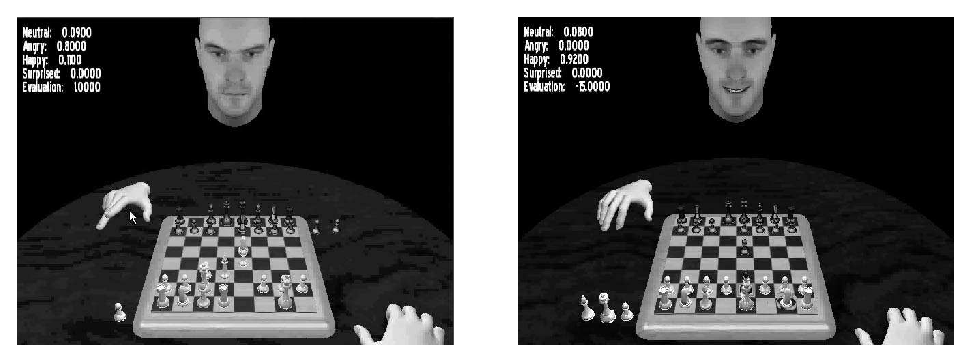
\includegraphics[width=\textwidth]{genimg-chess-emos-screens}
 
 \caption[Ukázka výrazů ve tváři hráče]{Ukázka výrazů ve tváři hráče při ztrátě pěšce (vlevo) a při sebrání dámy (vpravo). Převzato z \cite{AlvJoaCru-FuStMaAppEmoModEleGamCha}.} \label{img:ChessEmosScreens}
\end{figure}

Podobná technika je popsána v \cite{Hua+-LeaProbAutModChe}. Zde ovšem neslouží k popisu emocí hráče, ale predikci možného dalšího vývoje hry.

V \cite{FuLi-ForLeaAutAutGam} jsou učící automaty použity jako agenti v hře s nulovým součtem, která nemá jasné ekvilibrium, tj. vyvážený stav. Automaty se postupným hraním tahů učí a vylepšují svoji strategii tak, aby bylo dosaženo ekvilibria.

%%%%%%%%%%%%%%%%%%%%%%%%%%%%%%%%%%%%%%%%%%%%%%%%%%%%%%%%%%%%%%%%%%%%%%%%%%%%%%%
\subsection{Interakce s člověkem}
V \cite{HeiTri-SimEmoPerHumComInt} je prezentován prototyp systému pro modelování lidských emocí. Systém je založen na faktu, že velký vliv na emoce člověka má počasí. V jejich modelu pak konkrétně teplota vzduchu a množství světla. Oba tyto ukazatele popisují pomocí dvojice lingvistických proměnných, každá se třemi štítky. Navržený fuzzy automat je tvořen devíti stavy (odpovídající kombinacím hodnot těchto lingvistických proměnných).

Přechody mezi jednotlivými stavy prostředí poté modelují fuzzy automatem na základě změn počasí. Na základě aktuálního stavu automatu pak pomocí tzv. Plutchikova kola emocí určijí emoční stav pozorované osoby.


V \cite{Cas+-ProAutAspBasSenAna} pomocí pravděpodobnostních automatů analyzují tvrzení. U tvrzení sledují jeho tzv. polaritu, tedy zda je tvrzení míněno pozitivně, negativně nebo neutrálně). Každému slovu tvrzení je na základě slovníku přiřazena hodnota lingvistické proměnné \uv{polarita slova} se štítky např. \uv{velmi pozitivní}, \uv{pozitivní}, \uv{neutrální}, \uv{negativní} a \uv{velmi negativní}. Automat pak obsahuje stavy popisující možné stavy polarity tvrzení. Při zpracování pozitivního slova se automat přesouvá do stavu \uv{více} pozitivního, při negativním naopak a při neutrálním setrvává. Po zpracování celého tvrzení pak stav, ve kterém výpočet zkončil udává polaritu tvrzení.

V \cite{SchYou-ProSimHumMacDia} používají pravděpodobnostní automat pro řízení robotického pracovníka banky. Robot se ptá uživale v závislosti na tom, v jakém stavu se nachází (a na základě odpovědí svůj stav mění). Příkladem stavu automatu může být \uv{Uživatel si chce vybrat peníze}. Dotazy mohou být například \uv{Přejete si vybrat v Korunách?}, \uv{Přejete si vybrat v Eurech?} nebo \uv{Přejete si vrátit se k předchozí volbě?}.


%%%%%%%%%%%%%%%%%%%%%%%%%%%%%%%%%%%%%%%%%%%%%%%%%%%%%%%%%%%%%%%%%%%%%%%%%%%%%%%
\subsection{Sledování pohybu a aktivit osoby}
V \cite{TriHei-LinSumHumActSkiConAcc} je prezentován postup, jak pomocí sledování různých parametrů (pohyb získaný akcelerometrem a elektrická vodivost kůže) určit pravděpodobnou činnost (nicnedělání, chůze, práce, odpočinek) osoby. Ty jsou popsány lingvistickými proměnnými, které tvoří události automatu. Stavy automatu odpovídají aktivitám (např. odpočinek, pomalá chůze, běh). Pravidla jsou stanovena empiricky -- např. je pravděpodobnější, že člověk ze stavu nicnedělání přejde do stavu práce než do stavu běh.

Stejnou techniku využívají v \cite{Alv+-HumActRec+}. Zde však detekují činnosti: chůze, práce u sebe, hovor s kolegy, dávání si kávy, míting, a to pomocí polohy zařízení (chytrý telefon) (určené triangulací Wifi sítě) osoby a polohy těla. Poloha těla pak může být buď, že osoba stojí, sedí nebo jde. Tyto hodnoty jsou sledovány akcelerometrem, pohybovým čidlem, a gyroskopem. 

Podobnou techniku popisují v \cite{TurChe-MacRecHumActSur}. Zde však namísto fuzzy automatů používají pravděpodobnostní automat. Uvádějí však další aplikace pro tuto techniku, například identifikace pravděpodobného lupiče v bance.

%%%%%%%%%%%%%%%%%%%%%%%%%%%%%%%%%%%%%%%%%%%%%%%%%%%%%%%%%%%%%%%%%%%%%%%%%%%%%%%
\subsection{Průmyslové řídící systémy, fuzzy kontroléry}
Vztah fuzzy automatů a řídících systémů jsou popsány např. v \cite{HeKinSep-DecMakFuzEnvZUsOntCon+, Gra+-ApFuStFuOuFinMaPrRecVioOntAss, WeeFu-FormFuzAutAppModLeaSys, GraFodDri-HybFuzBooAutOntCont}. 

Systémy k modelování bývají často tak složité, že je obvykle nemožné popsat je zcela kompletně. Mohlo by tak například z důvodu chyby nebo neočekávaného vnějšího podnětu dojít k tomu, že model se octne v nekonzistením stavu, ze kterého nebude schopen se zotavit. Použití fuzzy automatů umožňuje do modelů určitou formu zotavení zanést.

V \cite{WeeFu-FormFuzAutAppModLeaSys, GraFod-FuzAutIntHybConSys} je fuzzy automat použit jako model pro návrh (obecných) řídících systémů. Řídící systém je stavový stroj, který je překlápěn mezi diskrétními stavy pomocí událostí. Řídící tak systém může být reprezentován automatem.

\TODO{vypsat z článků příklady}

V \cite{TzaRig-StaAnaAdaFuzzConSysUsiPetrNetLeaAut} používají učící se fuzzy událostmi řízené automaty, pro řízení výkonu při obloukovém svařování. Vstup automatu je realizován pomocí lingvistické proměnné \uv{naposledy bylo provedeno} se štítky \uv{zvýšení výkonu} a \uv{snížení výkonu}. Automat je sestaven tak, aby správně rozpoznával vhodné posloupnosti zvýšení a snížení výkonu za účelem zvýšení kvality sváru. 

V téže publikaci demonstrují obdobným způsobem uplatnění pro řízení robota pohybujícího se v neznámém prostředí. Systém sleduje změny rychlosti pohybu robota a na jejich základě řídí přidávání a ubírání výkonu tak, aby se robot v libovolném terénu pohyboval konstantní rychlostí.

%%%%%%%%%%%%%%%%%%%%%%%%%%%%%%%%%%%%%%%%%%%%%%%%%%%%%%%%%%%%%%%%%%%%%%%%%%%%%%%
\subsection{Problém městského růstu} \label{subs:UrbGrow}
Problém městského růstu je problém z oblasti urbanistiky. Řešením tohoto problému je co nejpřesnější predikce rozvoje městské zástavby na základě historických záznamů a současné situace. Ve zobecněné podobě se nemusí jednat jen o růst městské zástavby, ale například nárust vytíženosti silnic, kácení lesů nebo vytěženost ložisk. Stejně tak se nutně nemusí jednat o růst, ale obecný vývoj v čase. V této kapitole však budeme pro jednoduchost uvažovat standardní problém, tedy městský růst.

%\ T O D O{vyškrtat ne-fuzzy buněčné automaty}
Tento problém bývá často řešen pomocí buněčných fuzzy automatů. Věnují se jim např. v \cite{AlAhHep+-ModUrbGroDynUsCelAutGIS, Ahm+-CalFuzCelAutModUrbDynSauAr, War+-StoConCelModUrbGro, WhiEng-CelAutBasIntDynRegMod, LaiDraSch-IntMulEvCelAutMetLanSimMod, ManHatPra-FuzCelAutBasSheModUrGro+, ManHatPra-ModUrbGroUsFuzCelAut, Wu-CalStoCelAutAppRurUrbLanConv, PowSimWhi-HieFuzzPattMatcRegCompLanUseMap, Dra-CouFuzSetTheGisBaCelAutLanUseChaMod, WasPar-PreSpaDisEleEnCon+, LiuPhi-DevCelAutModUrbGroIncFuzSetApp}. V \cite{MraZimLapBaj-FuzCelAut+} podobnou technikou simulují šíření lesního požáru.

Problém bývá řešen obvykle tak, že sledovaná oblast (město) je rozděleno na parcely. Každá parcela je popsána obvykle několika ukazateli, např. jak moc je zastavěna či jak moc hluku parcela produkuje. Tyto ukazatele tvoří stav buňky bunečného automatu. Konfigurace automatu pak tedy popisuje celé město v určitý časový okamžik.

Přechodová pravidla pak mohou vypadat například:
\begin{itemize}
 \item Je-li vzdálenost parcely od centra města malá, pak růst zástavby bude velký
 \item Je-li vzdálenost od hlavní silnice velmi malá, pak růst zástavby bude malý a množství hluku bude velké
 \item Je-li vzdálenost od hlavní silnice velmi velká, pak růst zástavby bude malý
 \item Není-li lokalita atraktivní, pak růst zástavby bude malý
\end{itemize}

Ukázka vlivu různých pravidel na růst města je vyobrazena na obrázku \ref{img:VarTransRuls}. Na obrázku \ref{img:UrbGroProSample} je k vidění konkrétní ukázka městského růstu.

\begin{figure}
    \begin{subfigure}{0.9\textwidth}
      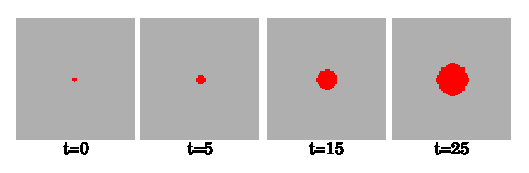
\includegraphics[width=\textwidth]{genimg-urban-growt-transitions-1}
      \caption{Růst města bez dalších dodatečných podmínek} 
    \end{subfigure}
    \\
    \begin{subfigure}{0.9\textwidth}
      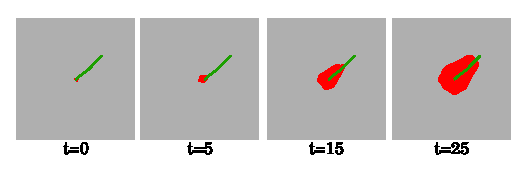
\includegraphics[width=\textwidth]{genimg-urban-growt-transitions-2}
      \caption{Růst města podél silnice} 
    \end{subfigure}
    \\
    \begin{subfigure}{0.9\textwidth}
      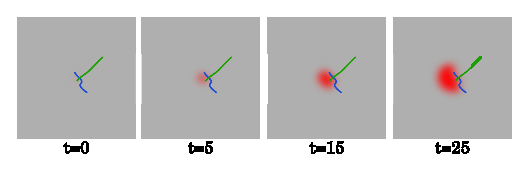
\includegraphics[width=\textwidth]{genimg-urban-growt-transitions-3}
      \caption{Růst města bržděn řekou} 
    \end{subfigure}

    \caption[Princip automatu pro problém městského růstu]{Ukázky chování automatu při různých počátečních konfiguracích. Šedě jsou znázorněny prázdné parcely, červeně zástavba, zeleně hlavní silnice a modře řeky. Převzato z \cite{LiuPhi-DevCelAutModUrbGroIncFuzSetApp}, upraveno.} \label{img:VarTransRuls}
\end{figure}

\begin{figure}
    \begin{subfigure}[t]{\textwidth}
      
\includegraphics[width=\textwidth]{genimg-urban-growt-city-1}
      \caption{Skutečný stav zástavby v uvedeném roce. Červená značí zástavbu, zelená přírodní oblasti (např. vodní plochy) a šedá nezastavěné plochy.} 
    \end{subfigure}
    \\
    \begin{subfigure}[t]{\textwidth} \centering
      
\includegraphics[width=\textwidth]{genimg-urban-growt-city-2}
      \caption{Simulovaný stav zástavby. Modrá značí zástavbu na počátku sledovaného období, červená značí (novou) zástavbu na konci sledovaného období, zelená přírodní oblasti (např. vodní plochy) a šedá nezastavěné plochy.} 
    \end{subfigure}

    \caption[Ukázky simulace městského růstu]{Ukázky simulace městského růstu. Převzato z \cite{Ahm+-CalFuzCelAutModUrbDynSauAr}.} \label{img:UrbGroProSample}
\end{figure}

%%%%%%%%%%%%%%%%%%%%%%%%%%%%%%%%%%%%%%%%%%%%%%%%%%%%%%%%%%%%%%%%%%%%%%%%%%%%%%%
\subsection{Další uplatnění}

V \cite{Maz+-ProTreAutAppBehMod} prezentují nástroj založený na pravděpodobnostních automatech, jehož úkolem je určovat nejpravděpodobnější aktivitu počítačového programu. Autoři mají k dispozici softwarový nástroj pro výpis nízkoúrovňového chování počítačového programu (např. systémová volání, změny na programovém zásobníku). Sledováním těchto informací při známém chování programu mohou stanovit vzory chování programu. Pravděpodobnostní automaty sestavené na základě těchto vzorů tak mohou modelovat chování programu. Automat tak například může předpovídat, že pokud program otevřel soubor, pak následující akcí bude s nejvyšší pravděpodobností alokace paměti na haldě.

V \cite{PedGac-LeaFuzzAut} navrhují používat učení fuzzy automatů pro konstrukci logických klopných obvodů. Tj. elektronických obvodů, které se na základě vstupů překlápí mezi různými diskrétními stavy. Autoři doporučují navrhovat elektronické takové obvody tak, že se dle očekávaného chování obvodu sestaví fuzzy automat (pomocí učení). Ten se poté \uv{zaokrouhlí}, tj. převede na bivalentní, a následně se sestaví odpovídající elektronický obvod.

%%%%%%%%%%%%%%%%%%%%%%%%%%%%%%%%%%%%%%%%%%%%%%%%%%%%%%%%%%%%%%%%%%%%%%%%%%%%%%%
%%%%%%%%%%%%%%%%%%%%%%%%%%%%%%%%%%%%%%%%%%%%%%%%%%%%%%%%%%%%%%%%%%%%%%%%%%%%%%%
%%%%%%%%%%%%%%%%%%%%%%%%%%%%%%%%%%%%%%%%%%%%%%%%%%%%%%%%%%%%%%%%%%%%%%%%%%%%%%%
\section{Zpracování obrazu} \label{cha:ImgProc}
Zpracování obrazu je velmi populární informatická disciplína. V této kapitole budou prezentovány některé problémy z této oblasti, které lze řešit pomocí fuzzy automatů. Vzhledem k tomu, že obraz bývá obvykle reprezentován bitmapou, bývá obraz obvykle zpracováván pomocí buněčných fuzzy automatů.

%%%%%%%%%%%%%%%%%%%%%%%%%%%%%%%%%%%%%%%%%%%%%%%%%%%%%%%%%%%%%%%%%%%%%%%%%%%%%%%
\subsection{Konvoluce} \label{subs:Convol}
Uvažujme obraz jako mřížku $m \times m$ pixelů s odstíny šedi jako hodnotami od $0$ do $1$. Hodnota $0$ značí černou, hodnota $1$ bílou. Jinými slovy, o pixelu můžeme hovořit jako o ligvistické proměnné \uv{pixel má bílou barvu}.

Každý obraz tak můžeme považovat za konfiguraci buněčného fuzzy automatu. Návrhem vhodné přechodové funkce tak můžeme vytvořit automat, který provádí určitou operaci pro úpravu obrazu. Typickou operací je tzv. obrazový filtr, což je zobrazení které obrazu přiřazuje jiný obraz stejných rozměrů.

Speciálním případem filtru je konvoluce \cite{Rus-ImaProHan}. Konvoluce je v základu obrazový filtr, který přiřazuje (novou) hodnotu pixelu na základě váženého součtu (stávající) hodnoty pixelu a hodnot pixelů sousedních. Váhy bývají reprezentovány tzv. konvoluční maticí. Například matice
$$
  B = \begin{pmatrix}
       1 & 2 & 1 \\
       2 & 4 & 2 \\
       1 & 2 & 1 
      \end{pmatrix}
$$
je konvoluční maticí jednoduchého rozostření. Konvoluční matice se aplikuje následujícím způsobem:
$$
  c'_{i,j} = \frac{1}{S} \; \sum_{\mathclap{k,l \in \{-1, 0, +1\}}} \; B_{k+1, l+1} c_{i+k, j+l}
$$
kde $c_{i,j}$ je pixel původního obrazu, $c'_{i,j}$ je pixel nového a $S$ je součet hodnot v matici $B$.

Další ukázkou grafického filtru pracujícího s využitím buněčného fuzzy automatu je například filtr pro zvýraznění tvarů. Je daný následujícím předpisem
$$
  c'_{i,j} = \max(0, \min(1, 
    \begin{dcases}
      \epsilon (c_{i,j} + 1) - 1	& \text{pokud $c_{i,j} > neighs_{i,j}$} \\
      \epsilon c_{i,j}			& \text{pokud $c_{i,j} < neighs_{i,j}$} \\
      c_{i,j}	& \text{pokud $c_{i,j} = neighs_{i,j}$} 
    \end{dcases}
    ))
$$
kde $\epsilon > 1$ je parametr udávají agresivitu zvýrazňování a $neighs_{i,j}$ je součet hodnot okolních buňek.

Ukázky aplikací obou filtrů jsou k nalezení na obrázku \ref{img:Filters}. V následujících podkapitolách budou prezentovány některé další (pokročilejší) techniky zpracování obrazu využívající buněčné fuzzy automaty.

\begin{figure}
 
\includegraphics[width=\textwidth]{genimg-filters}
 
 \caption[Ukázky jednoduchých filtrů]{Ukázky jednoduchých filtrů. Vlevo původní obrázek, uprostřed obrázek po $5$ generacích jednoduchého rozostřovacího filtru a vpravo obrázek po $8$ generacích filtru pro zvýraznění tvarů ($\epsilon = 1{,}1$). Původní obrázek převzat z \cite{web-Lenna}.} \label{img:Filters}
\end{figure}

%%%%%%%%%%%%%%%%%%%%%%%%%%%%%%%%%%%%%%%%%%%%%%%%%%%%%%%%%%%%%%%%%%%%%%%%%%%%%%%
\subsection{Hledání hran}
Hledání hran je jednou ze základních technik zpracování obrazu. Hledání hran je často klíčové pro rozpoznávání vzorů v obrazech. V dnešní době existuje značné množství technik pro rozpoznávání hran \cite{MaiAgg-StuComVarImDetEdTec}. V \cite{MarMeySol-HybMetGasDifModFuzCelAutImSha} je popsán poměrně elegantní způsob, jak hledání hran vyřešit pomocí buněčných fuzzy automatů. V \cite{PatMor-EdgDetTecFuzzLogCEllLeaAutFuzzImPro} pak tuto techniku vylepšují pomocí strojového učení.

Označme osmici směrů dle obrázku \ref{img:Directions:8Directions} jako $H$, $LH$, $L$, $LD$, $D$, $PD$, $P$ a $PH$. Množinu těchto směrů označme $dim$. Dále označme $c_X$ (kde $X \in dim$) jako sousední buňku buňky $c$ ve směru $X$.

\begin{figure}
   \begin{subfigure}[t]{0.4\textwidth}
      \includegraphics[width=\textwidth]{mpimg-rest4}
      \caption{8 směrů}  \label{img:Directions:8Directions}
    \end{subfigure}%
%
    \begin{subfigure}[t]{0.4\textwidth}
      \includegraphics[width=\textwidth]{mpimg-rest5}
      \caption{Ukázka hrany procházející buňkou. Ve směru $H$ (červené šipky) prochází hrana, ve směru $P$ (zelené šipky) neprochází.}  \label{img:Directions:Edges}
    \end{subfigure}
\end{figure}

Rozpoznávání hran vychází z následujcí úvahy: Má-li buňka $c_X$ výrazně jinou barvu, než buňka $c$, pak buňkou $c$ prochází hrana ve směru $X$ (červené šipky v obrázku \ref{img:Directions:Edges}). Má-li buňka $c_X$ velmi podobnou barvu než buňka $c$, pak buňkou $c$ neprochází hrana ve směru $X$ (zelené šipky v obrázku \ref{img:Directions:Edges}). 

Pomocí těchto pravidel tak lze sestavit buněčný fuzzy automat, který rozpoznává hrany. 

Dle \cite{MarMeySol-HybMetGasDifModFuzCelAutImSha} může být hodnota lingvistické proměnné \uv{buňkou $c$ prochází hrana} dále použita pro zaostřování obrazu.

%%%%%%%%%%%%%%%%%%%%%%%%%%%%%%%%%%%%%%%%%%%%%%%%%%%%%%%%%%%%%%%%%%%%%%%%%%%%%%%
\subsection{Ostraňování šumu} \label{subs:NoisRem}
Odstraňování šumu je další častý problém, který je třeba při zpracování obrazů řešit. Pro studium technik odstraňování šumu se používá typicky zašumnění tzv. impulzním šumem popř. šumem \uv{sůl a pepř}. Zašumnění impulzním šumem nahradí stanovený počet pixelů náhodnými barvami. Šumění \uv{sůl a pepř} pak narazuje pixely buď bílou ($1$) nebo černou ($0$) barvou.

V \cite{SadRetKam-EfMetImpNoiRedImFuzCelAut} je prezentována jednoduchá avšak efektivní technika, která kombinuje klasický bivalentní buněčný automat s buněčnýcm fuzzy automatem. 

V první fázi je klasickým buněčným automatem šum detekován. Buňka obsahuje šum, pokud rozdíl její barvy od průměrné barvy jejich sousedů překračuje stanovenou mez. Tato mez může být stanovena statisticky, například na základě směrodatné odchylky barev pixelů celého obrazu. V druhé fázi je aplikován buněčný fuzzy automat, který buňky obsahující šum nahradí hodnotami spočtenými z jejich okolí. Ukázky výsledků jsou na obrázku \ref{img:Noises}. 

\begin{figure}

  
\includegraphics[width=\textwidth]{genimg-noises}
    
  \caption[Ukázka odstraňování šumu]{Ukázka odstraňování šumu. Vlevo původní obraz, uprostřed zašumněn (šumem sůl a pepř), vpravo po $6$ generacích filtru na ostranění šumu. Původní obrázek převzat z \cite{web-Lenna}.} \label{img:Noises}
\end{figure}

Velmi podobný způsob ostranění šumu je popsán v \cite{SahUguSah-SalPepNoiFilFuzCelAut}. Zde však operace detekce šumu a jeho odstranění provádějí v jednom kroku.

%%%%%%%%%%%%%%%%%%%%%%%%%%%%%%%%%%%%%%%%%%%%%%%%%%%%%%%%%%%%%%%%%%%%%%%%%%%%%%%
\subsection{Rozpoznávání jednoduchých vzorů} \label{subs:SimpImgRec}

Ropoznávání vzorů je další z častých způsobů práce s obrazy. Obecně je problém definován (obdobně, jako rozpoznávání textových vzorů v kapitole \ref{sec:Rec}) jako problém určení, zda-li obraz obsahuje předem stanovený vzor či ne. Obvykle nás také zajímá, kde přesně se vzor v obraze vyskytuje.

V \cite{MajCha-FuzCelAutModPatClas} je popsán způsob, který popisuje rozpoznávání vzorů v obrazu velikosti $1 \times m$ pomocí (jednodimenzionálního) buněčného automatu. Automat pracuje s lingvistickou proměnnou \uv{pixel má šedou barvu}, která má několik štítků (reprezentující různé stupně šedi). Přechodová pravidla jsou navžena tak, aby rozpoznávaný (a případně jemu podobný) vzor zvýrazňovala. Přechodová pravidla však obvykle bývají tvořena všemi kombinacemi odstínů pro všechny sousední buňky, čímž značně roste její mohutnost. Tato technika je proto prakticky nepoužitelná.

Zcela jiný přístup pužívají v \cite{WanJiaZhoDu-ImProcBasFuzCelAuMod}. Vzor nepovažují za konkrétní kombinaci odstínů barev, ale jako část obrazu splňující určité vlastnosti. Konkrétně, skvrny jednolité barvy, které jsou obklopeny různorodě zabarvenou plochou. Podrobnější popis (včetně ukázky výstupů) je uveden v kapitole \ref{subs:MedImgs}.

%%%%%%%%%%%%%%%%%%%%%%%%%%%%%%%%%%%%%%%%%%%%%%%%%%%%%%%%%%%%%%%%%%%%%%%%%%%%%%%
\subsection{Složené geometrické útvary} \label{subs:CompGeoms}

V \cite{Lee-FuzTreAutSynPatRec} byl popsán způsob, jak pomocí fuzzy tree automatů rozpoznávat složené geometrické útvary. Složený geometrický útvar je chápán jako S-term, jehož listové S-termy reprezentují \uv{primitivní geometrické objekty} (čtverec, kruh, trojúhelník, aj.). Jeho vnitřní S-termy pak popisují vzájemný vztah či vlastnost (např. vzájemnou polohu) jednotlivých podobjektů. Na obrázku \ref{img:Geoms} je vyobrazena ukázka složeného geometrického útvaru vyobrazující \uv{budovu kostela} a stromová reprezentace jemu odpovídajícího S-termu.

%\begin{example}[Složený geometrický útvar]
%\end{example}

\begin{figure} 
 \begin{subfigure}{0.4\textwidth}
  \includegraphics{mpimg-rest6}
 \end{subfigure}
 %
 \begin{subfigure}{0.4\textwidth}
  \includegraphics{mpimg-rest7}
 \end{subfigure}
 
 \caption[Příklad složeného geometrického tvaru]{Příklad složeného geometrického tvaru a stromová reprezentace jemu odpovídajícímu S-termu. Symbol $t$ reprezentuje trojúhelník, symbol $o$ obdélník, symbol $c$ čtverec. S-term $N(t_1 t_2)$ symbolizuje \uv{$t_1$ je nad $t_2$} a $V(t_1 t_2 t_3)$ značí \uv{$t_1$, $t_2$ a $t_3$ leží vedle sebe}.} \label{img:Geoms}
\end{figure}

Mějme primitivní geometrický tvar $x$. Pak tento tvar je čtvercem, pokud je tvořen čtveřicí bodů a všechny jeho vnitřní úhly jsou pravé. Vlastnost \uv{být pravý úhel} můžeme snadno vyjádřit ve stupních pravdivosti. Tedy, že úhel $\pi/2$ je pravým ve stupni $1$ a například úhel $\pi$ v nulovém stupni. Díky tomu můžeme i vlastnost \uv{být čtvercem} uvažovat se stupni pravdivosti.

Obdobným způsobem můžeme popsat různé další primitivní geometrické tvary. Stejně tak můžeme stanovit stupně pravdivosti pro vlastnosti např. \uv{geometrický tvar $x$ má neprázdný průnik s geometrickým tvarem $y$} či \uv{geometrické tvary $x$ a $y$ jsou přímky a jsou navzájem rovnoběžné}.

Na základě těchto popisů může být navržen automat, který S-termy reprezentující geometrické tvary rozpoznává a to včetně geometrických tvarů \uv{podobných} vzoru.

%%%%%%%%%%%%%%%%%%%%%%%%%%%%%%%%%%%%%%%%%%%%%%%%%%%%%%%%%%%%%%%%%%%%%%%%%%%%%%%
\subsection{Detekce požárů}
V \cite{HamKoNam-FirFlaDetBasFuzFinAut, KoHamNam-ModForFuFiAuDetIrrFirFla} používají fuzzy automaty pro rozpoznávání vzorů ve videosekvenci, konkrétně pro detekci požárů.

V první fázi se snímek rozdělí na několik regionů. Je-li region tvořen teplými a světlými barvami, je označen jako tzv. kandidát. Pro každého kandidáta je pak sestaven fuzzy automat o čtyřech stavech $q_{VM}, q_{M}, q_{P}, q_{VP}$. Pokud se automat regionu nachází ve stavu $q_{VM}$, znamená to, že \uv{region je velmi málo pravděpodobně tvořen plamenem}. Obdobně pro $q_{M}$ (\uv{málo pravděpodobně}), $q_{P}$ (\uv{hodně pravděpodobně}) a $q_{VP}$ (\uv{velmi pravděpodobně}). Abecedou událostí jsou pak kombinace dalších atributů (svit, pohyb v určitém směru, vlnění) spočtených z předchozích snímků. Přechodové pravidlo pak může být např. \uv{pokud je region ve stavu $q_{P}$ a došlo k velkému posunu směrem nahoru a malému snížení svitu, pak přejdi do stavu $q_{VP}$}. Přesně byla přechodová funkce navržena statistickým pozorováním známých videosekvencí s požáry.

%%%%%%%%%%%%%%%%%%%%%%%%%%%%%%%%%%%%%%%%%%%%%%%%%%%%%%%%%%%%%%%%%%%%%%%%%%%%%%%
%%%%%%%%%%%%%%%%%%%%%%%%%%%%%%%%%%%%%%%%%%%%%%%%%%%%%%%%%%%%%%%%%%%%%%%%%%%%%%%
%%%%%%%%%%%%%%%%%%%%%%%%%%%%%%%%%%%%%%%%%%%%%%%%%%%%%%%%%%%%%%%%%%%%%%%%%%%%%%%
\section{Biologie a medicína}

Biologie a medicína jsou odvětví, které zpravidla disponují velikým množstvím dat, které je třeba zpracovat. Typicky, v datech získaných nějakým sledováním či měřením najít výskyt nějakého vzoru. Fuzzy popř. pravděpodobnostní automaty mohou být v této oblasti nápomocny.

Vzhledem k tomu, že většina biologických a medicínských uplatnění vyžaduje znalost dané problematiky, budou tato uplatnění rozebrána jen zevrubně.

%%%%%%%%%%%%%%%%%%%%%%%%%%%%%%%%%%%%%%%%%%%%%%%%%%%%%%%%%%%%%%%%%%%%%%%%%%%%%%%
\subsection{Rozpoznávání řetězců DNA} \label{subs:DNA}
Řetězec DNA je organická makromoleukula deoxyribonukleové kyseliny. Je tvořena sekvencí tzv. nukleotidů. Každý nukleotid obsahuje jednu ze čtyř nukleových bází, adeninu, guaninu, cytosinu a nebo thyminu. Nukleové báze se často značí po řadě $A$, $G$, $C$ a $T$ a celá DNA tak může být zapsána jako řetězec těchto symbolů.

Řetězce DNA často kódují základní informace o živých organizmech a je proto snaha pochopit její strukturu. Popis využití fuzzy a pravděpodobnostních automatů na rozpoznávání řětězců DNA je uveden v \cite{SnaKepAbrHas-AproxStriMatchFuzzAut, Ron-AutLeaApp, ZlaSteSch-FiStaConTraFemPro, Her-ProAriAutAppSoComFraBioSeqAna}. 

%%%%%%%%%%%%%%%%%%%%%%%%%%%%%%%%%%%%%%%%%%%%%%%%%%%%%%%%%%%%%%%%%%%%%%%%%%%%%%%
\subsection{Biologické simulace}
V \cite{CheMyn-ModAlgBloDutCosWat+} je prezentován model založený na buněčných fuzzy automatech modelující růst mořských řas. Funguje na velmi podobném principu jako problém městského růstu (viz kapitola \ref{subs:UrbGrow}).

V \cite{MilAtl-ProAuModEpiCelNet} používají pravděpodobnostní automaty na simulaci živého ogranizmu. Princip je podobný, jak u buněčných automatů, jen model není založen na pevné mřížce, ale buňky vznikají a mizí. Každá buňka se nachází v některém stavu z množiny stavů (jako je např. \uv{buňka se zrodila}, \uv{buňka je přípravena k dělení}, \uv{buňka je rodičovskou buňkou jiné buňky}). Přechodová pravidla mohou vypadat například následovně: je-li buňka \uv{připravena k dělení}, pak v dalším kroku provede dělení, tj. vytvoří novou buňku ve stavu \uv{buňka se zrodila} a buňka samotná přechází do stavu \uv{buňka je rodičovskou buňkou jiné buňky}. Díky využití pravděpdobnostních automatů se takovéto modely mohou značně více přiblížit reálným buněčným sítím.

V \cite{BocChe-CriBePrAuNetModSprInfDis+} používají systém podobný pravděpodobnostnímu buněčnému automatu pro modelování šíření infekčních nemocí. Každá buňka je buďto prázdná nebo se v ní nachází osoba. Osoba může být ve stavu \uv{nenakažena} nebo \uv{nakažena}. Nachází-li se v okolí \uv{nenakažené} osoby alespoň jedna \uv{nakažená} osoba, pak s určitou pravděpodobností přejde při dalším časovém kroku do stavu \uv{nakažena}, jinak zůstává ve stavu \uv{nenakažena}. 

Autoři navíc do modelu zanášejí pohyb jedinců, tj. že s určitou pravděpodobností se může osoba přesunout na některou sousední buňku je-li neobsazena. Změnou parametrů systému (jednotlivých pravděpodobností) tak lze nasimulovat vymícení choroby nebo naopak vznik epidemie.

%%%%%%%%%%%%%%%%%%%%%%%%%%%%%%%%%%%%%%%%%%%%%%%%%%%%%%%%%%%%%%%%%%%%%%%%%%%%%%%
\subsection{Analýza zdravotního stavu pacienta}
V \cite{Jia+-ExHeaSimMetBasIntHumTheMod, GupRah-CliMonUsFuzSys, CamMerNun-UsFuzAutDiagPrHeaPro, SteAdl-CliMonFuzAut} jsou popisovány způsoby, jak pomocí fuzzy automatů sledovat zdravotní stav pacienta. 

Technika pracuje s událostmi řízeným fuzzy automatem. Stavy automatu v tomto případě reprezentují choroby (popř. stádia jedné choroby), přechodová funkce pak přechody mezi nimi. Přechodová pravidla pak popisují přechody při různých událostech či akcích (např. medikace). 

Tato technika tak může sloužit k porovnávání simulovaného a skutečného stavu (např. po medikaci, zákroku) pacienta a případně včas reagovat na odchylku. Výhodou této techniky je, že značně zjednodušuje sledování více diagnóz současně.

V \cite{CamMerNun-UsFuzAutDiagPrHeaPro} se fuzzy automaty používají pro diagnózu srdečních chorob. Po spuštění automat na základě pohlaví a věkové skupiny přejde do odpovídajícího podautomatu. Ten si poté sám žádá měření různých parametrů (aktuální tepová frekvence, aktuální variabilita srdeční frekvence) v závislosti na tom, kdy je který pro proces diagnózy aktuálně potřebný. V případě stanovení rizika je riziko ohlášeno a automat se vrací do počátečního stavu a proces se spouští znovu (aby diagnózu ověřil). 

V \cite{GupRah-CliMonUsFuzSys} tuto techniku používají pro sledování systolického krevního tlaku a množství krevního cukru. V \cite{Jia+-ExHeaSimMetBasIntHumTheMod} používají podobnou techniku pro sledování těla při sportu (konkrétně tělní teplotu, dehydrataci a srdeční tep).


%%%%%%%%%%%%%%%%%%%%%%%%%%%%%%%%%%%%%%%%%%%%%%%%%%%%%%%%%%%%%%%%%%%%%%%%%%%%%%%
\subsection{Analýza lékařských snímků} \label{subs:MedImgs}
V \cite{Est+-CytImAnaGenFuFiStMa} využívají učící se fuzzy automat pro rozpoznávání zhoubných (maligních) nádorových buněk. Vstupem této techniky je mikroskopický snímek z buněk z prsní tkáně, výstupem pak nalezené maligní buňky. Využívají faktu, že nezhoubné buňky mají na snímcích obvykle symetričtější tvary a obsahují méně \uv{skvrn}.

Proces rozpoznávání probíhá následujícím způsobem:
\begin{itemize}
 \item Snímek je převeden do odstínů šedi.
 \item Jednotlivé buňky na snímku jsou izolovány do samostatných obrazů. Následně jsou zpracovávány všechny obrazy postupně.
 \item Na obraze jsou rozpoznány plochy stejné nebo podobné barvy.
 \item Z ploch je na základě relace \uv{plocha $X$ obsahuje plochu $Y$} zkonstruován strom ploch.
 \item Strom je následně zakódován do řetězce a rozpoznán fuzzy automatem.
\end{itemize}

Strom je do řetězce kódován tak, že strom je projit průchodem do šířky a každému uzlu je přiřazen symbol odpovídající počtu jeho potomků. Automat, který tyto řetězce rozpoznává, byl sestaven učením z veřejné databáze snímků.

V \cite{WanJiaZhoDu-ImProcBasFuzCelAuMod} popisují, jak pomocí buněčných fuzzy automatů rozpoznávat folikuly\footnote{Folikula je dutinka ve vaječníku, v níž probíhá zrání vajíčka. \cite{web-Folikul}} v ultrazvukových snímcích vaječníků. Poukazují na to, že folikula je na snímku tvořena jednolitou skvrnou stejné barvy, obklopena ostatní tkání (různorodě zabarvená plocha).

Automat v první fázi vyhledává kandidáty na folikuly. Ty posléze automat zvýrazňuje. Na obrázku \ref{img:Follicles} jsou k nahlédnutí ukázky rozpoznaných folikul pomocí této techniky.

\begin{figure}
  \begin{subfigure}[t]{\textwidth}
    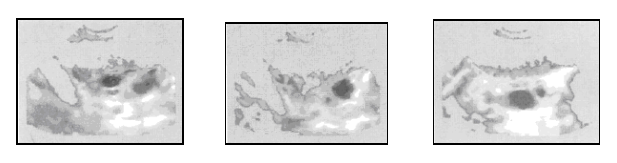
\includegraphics[width=\textwidth]{genimg-follicles-1}
    \caption{Ultrazvukové snímky vaječníků} \label{img:Follicles:Screens}
  \end{subfigure}
  \\
  \begin{subfigure}[t]{\textwidth}
    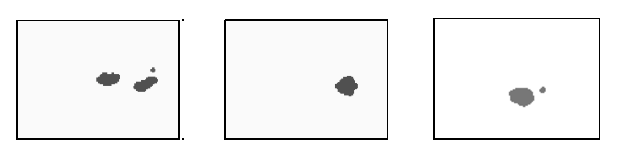
\includegraphics[width=\textwidth]{genimg-follicles-2}
    \caption{Rozpoznané folikuly}
  \end{subfigure}
 
  \caption[Ukázky rozpoznávání folikul]{Ukázky rozpoznávání folikul. Převzato z \cite{WanJiaZhoDu-ImProcBasFuzCelAuMod}, upraveno.} \label{img:Follicles}
\end{figure}

V \cite{PatPal-FuzGraSynRecSkeMatXra} popisují způsob, jak pomocí fuzzy automatů sledovat vývoj kostí ruky dítěte. Z R\"{o}ntgenového snímku ruky pomocí detekce hran obrdrží obrysy kostí. Ty pak pomocí techniky podobné rozpoznávání složených geometrických tvarů (kapitola \ref{subs:CompGeoms}) používají k určování stádia vývinu patřičné kosti.

%%%%%%%%%%%%%%%%%%%%%%%%%%%%%%%%%%%%%%%%%%%%%%%%%%%%%%%%%%%%%%%%%%%%%%%%%%%%%%%
\subsection{Další aplikace} \label{subs:BioMedRest}
V \cite{PedGac-LeaFuzzAut}, popř. i \cite{RigTza-FuzAutFauDia} analyzují elektrokardiogram (EKG), tj. záznam srdeční aktivity v čase. Využivají při tom techniky uvedené v kapitole \ref{subs:RozpSign}. Model dokáže sledovat činnost srdečního cyklu a případně detekovat např. srdeční arytmie.

\TODO{příklad?}

V \cite{Alv-HumGaiModUsGenFuzFinStaMac} (popř. i \cite{AlvTri-ComModQuaPerSig})
používají fuzzy automaty pro modelování fungovaní protézy dolní končetiny. Pomocí akcelerometrů sledují pohyb patřičné náhrady a pomocí známých vzorů spouštějí automat, který určuje, v jaké fázi pohybu protéza je.

%%%%%%%%%%%%%%%%%%%%%%%%%%%%%%%%%%%%%%%%%%%%%%%%%%%%%%%%%%%%%%%%%%%%%%%%%%%%%%%
%%%%%%%%%%%%%%%%%%%%%%%%%%%%%%%%%%%%%%%%%%%%%%%%%%%%%%%%%%%%%%%%%%%%%%%%%%%%%%%
%%%%%%%%%%%%%%%%%%%%%%%%%%%%%%%%%%%%%%%%%%%%%%%%%%%%%%%%%%%%%%%%%%%%%%%%%%%%%%%
\section{Implementace vybraných problémů}
V rámci této práce byly vybrané aplikace naimplementovány. Tato kapitola popisuje základní informace o způsobu, jak byly tyto aplikace naimplementovány.

Studium této kapitoly předpokládá alespoň základní znalost objektového programování, nejlépe pak znalost programovacího jazyka Java.

%%%%%%%%%%%%%%%%%%%%%%%%%%%%%%%%%%%%%%%%%%%%%%%%%%%%%%%%%%%%%%%%%%%%%%%%%%%%%%%
\subsection{Základní informace}
Aplikace byly implementovány v programovacím jazyce Java na platformě Java Standart Edition. Projekt byl strukturován tak, aby bylo možné jej automaticky sestavit a spustit pomocí nástroje Apache Maven \cite{web-Maven}. Pro jeho sestavení a spuštění nejsou potřebné žádné dodatečné nástroje či knihovny. Implementace by měla být platformově nezávislá, vyvíjena a testována byla na platformě GNU/Linux.

Samotný projekt je rozdělen na moduly (podprojekty) odpovídající použitému typu automatu, tj. \verb|fuzzy-automata| (nedeterministický fuzzy automat), \verb|event-driven-fuzzy-automata| (událostmi řízený fuzzy automat), \verb|fuzzy-tree-automata| (fuzzy tree automat) a \verb|cellular-fuzzy-automata| (buněčný fuzzy automat). Pravděpodobnostní automaty implementovány nebyly.

Každý z těchto modulů obsahuje vždy základní, abstraktní, třídu implementující definici patřičného automatu (tj. datovou strukturu). Dále pak obsahuje třídu, která je jejím potomkem a rozšiřuje ji o implementaci vybraných algoritmů (např. výpočet, determinizace a podob.).

Každý modul je koncipován jako softwarová knihovna. Pro snažší použití však každý modul obsahuje obvykle několik spustitelných tříd (tj. tříd s metodou \verb|main|), které zaobalují vybranou funkcionalitu modulu do spustitelného programu. Každý modul zpravidla obsahuje také adresář \verb|test-data| obsahující testovací data.

Implementované aplikace jsou umístěny v modulech podle typu automatu, se kterým pracují. Každá aplikace je implementována (obvykle) samostatnou třídou a obsahuje patřičné spustitelné třídy a testovací data.

Projekt dále obsahuje modul \verb|core|, který implementuje základní funkcionalitu společnou pro všechny moduly. Tedy implementaci abeced, symbolů, řetězců, fuzzy množin a relací a podob. Implementuje také tzv. \textsc{TIMFile}, což je speciální formát souboru navržený pro vstup a výstup dat z aplikace.

Veškeré podrobnější informace jsou k nalezení v javadoc dokumentaci v samotném kódu, popř. v \textsc{README} souborech jednotlivých modulů. Nyní budou ve stručnosti popsány jednotlivé aplikace, které byly implementovány.

%%%%%%%%%%%%%%%%%%%%%%%%%%%%%%%%%%%%%%%%%%%%%%%%%%%%%%%%%%%%%%%%%%%%%%%%%%%%%%%
\subsection{Korekce překlepů}
Detekce a korekce překlepů byla implementována na základě popisu v kapitole \ref{subs:DetTyp}. Realizuje ji třída \verb|TyposCorrecter| a spouští se pomocí \verb|TyposCorrecterApp|. Proces korekce je konfigurován slovníkem (seznam korektních slov), popisem klávesnice a stupni, v jakých má být akceptován stisk právě jedné extra klávesy, stisk více extra kláves, stisk jiné klávesy či vynechání klávesy.

Instance třídy \verb|TyposCorrecter| bere na svém vstupu textový řetězec tvořený jedním nebo více slovy oddělených mezerou. Výstupem je posloupnost slov dle následujího klíče:
\begin{enumerate}
 \item výstupem je slovo $x$, jestliže je vstupní slovo $x$ ve slovníku
 \item výstupem je slovo $y$, jestliže je vstupní slovo $x$ nejpodobnější slovu $y$, které je ve slovníku
 \item výstupem je slovo $x$, pokud žádné slovo ze slovníku mu není podobné
\end{enumerate}

Podobnost řetězců je počítána pomocí deformovaných automatů rozpoznávající slova ze slovníku. Ukázka korekce překlepů (při výchozím nastavení) je uvedena v tabulce \ref{tab:TyposOut}. Jak je v tabulce vidět, program má problém s krátkými slovy, avšak u dlouhých slov dokáže obnovit i velmi \uv{poškozené} slovo.

\begin{table}
 \centering
  \begin{tabular}{|l||l|l|l|l|l|l|l|l|l|}
    \hline
    vstup 	& februacy & jaruanry & devmber  & october & asdbril	\\\hline
    výstup 	& february & january  & december & october & april	\\\hline
    \hline
    vstup 	& maj   & jana & poctober & asauguszt  & mnobmvmert	\\\hline
    výstup	& march & may  & october  & august     & november	\\\hline
  \end{tabular}

 \caption[Ukázka korekce překlepů]{Ukázka korekce překlepů při slovníku anglických názvů měsíců} \label{tab:TyposOut}
\end{table}

%%%%%%%%%%%%%%%%%%%%%%%%%%%%%%%%%%%%%%%%%%%%%%%%%%%%%%%%%%%%%%%%%%%%%%%%%%%%%%%
\subsection{Rozpoznávání ručně psaného textu}
Rozpoznávání ručně psaného textu bylo naimplementováno dle kapitoly \ref{subs:RecHandWrit}. Tato aplikace je naimplementována jako interaktivní grafická aplikace spouštěná třídou \verb|HandwrittenTextGuiApp|. 

V prostřední části okna aplikace se nachází plátno, kde je možno pomocí tahu myší psát. Na plátně se červeně zvýraznůjí body, ve kterých se lámou segmenty. Ve stavovém řádku se zobrazuje řetězec, který napsanému tvaru odpovídá. V levé části okna se nachází tabulka s automaty a stupni pravdivosti, jak moc je jimi napsaný tvar přijímán. Nástrojová lišta pak obsahuje prvky pro konfiguraci a ovládání programu. Parametr \textit{Shake reduction} udává minimální délku segmentu, zaškrtávací tlačítko \textit{Immediate} zapíná automatické spuštění výpočtu při uvolnění tlačítka myši.

Seznam automatů se zadává při spuštění programu. Pro vygenerování automatu rozpoznávající vzor a jeho následnou deformaci lze použít spustitelné třídy \verb|AutomatonOfWordApp| a \verb|DeformAutomatonApp|. Pro testování bylo v adresáři s testovacími daty vytvořeno $10$ vzorů odpovídající číslicím $0$ až $9$ (každá ve více variantách). 

Ukázka okna aplikace je na obrázku \ref{img:HandWritScreen}.

\begin{figure}
 \centering
 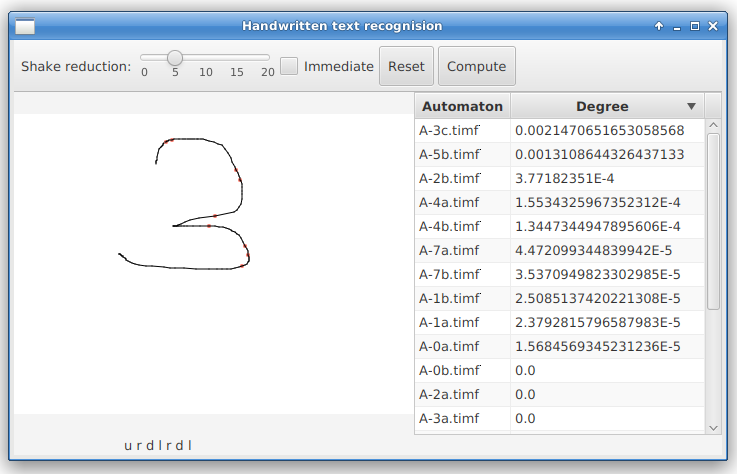
\includegraphics[width=0.8\textwidth]{genimg-handwritrec-screen}
 \caption{Ukázka aplikace pro rozpoznávání ručně psaného textu} \label{img:HandWritScreen}
\end{figure}

%%%%%%%%%%%%%%%%%%%%%%%%%%%%%%%%%%%%%%%%%%%%%%%%%%%%%%%%%%%%%%%%%%%%%%%%%%%%%%%
\subsection{Detekce úplných $m$-árních stromů}
Detekce úplných $m$-árních stromů je naimplementována pomocí fuzzy tree automatů a to dle kapitoly \ref{subs:DetComTrees}. V adresáři s testovacími daty se nachází vzorové stromy pro úplný ternární a kvadrární strom. Testování se spouští třídou \verb|TreeOnFTaRunner|.

%%%%%%%%%%%%%%%%%%%%%%%%%%%%%%%%%%%%%%%%%%%%%%%%%%%%%%%%%%%%%%%%%%%%%%%%%%%%%%%
\subsection{Simulace spotřeby elektrického produdu}
Simulace spotřeby elektrického proudu byla naimplementována dle kapitoly \ref{subs:MonElComNet}. Výpočet realizuje třída \verb|PowerConsumptionComputer|. Jejím vstupem jsou informace o spotřebičích v síti, jejich možných stavech a spotřebách. Dále pak seznam naměřených spotřeb elektrického proudu a dodatečné parametry. 

Pomocí třídy \verb|PowerConsumptionsToFEDA| jsou tato data transformována na fuzzy událostmi řízený automat a sekvenci fuzzy událostí. Automat je posléze spuštěn s těmito událostmi a výsledný stav je opět převeden na informace o spotřebičích a jejich stavech. 

%%%%%%%%%%%%%%%%%%%%%%%%%%%%%%%%%%%%%%%%%%%%%%%%%%%%%%%%%%%%%%%%%%%%%%%%%%%%%%%
\subsection{Zpracování obrazu}
Naimplementovány byly také vybrané techniky pro zpracování obrazu. Realizovány byly pomocí buněčných fuzzy automatů. Pro import a export (převod mezi bitmapou a souborem konfigurace buněčného automatu) je slouží spustitelná třída \verb|ImageConfigConverter|.

Byly implementovány některé grafické filtry uvedené v kapitole \ref{subs:Convol}. Třída \verb|ConvolutionalCFA| implementuje automat realizující obecnou konvoluci. Třída \verb|SimpleBlurFilterAutomaton| pak pomocí konvoluce implementuje jednoduché rozostření. Třída \verb|MyBEFilterAutomaton| implementuje BE filtr. 

Třída \verb|NoiseReductionAutomaton| implementuje metodu pro odstranění šumu z obrazu popsanou v kapitole \ref{subs:NoisRem}. Pro přidání šumu do obrázku je možné použít spustitelnou třídu \verb|ConfigNoiserTool|.

Ukázky výstupů jsou na obrázcích \ref{img:Filters} a \ref{img:Noises}.

%%%%%%%%%%%%%%%%%%%%%%%%%%%%%%%%%%%%%%%%%%%%%%%%%%%%%%%%%%%%%%%%%%%%%%%%%%%%%%%
\subsection{Metoda lisování dat} \label{subs:DataPresImpl}

Metoda lisování dat byla popsána v kapitole \ref{subs:DataPresTech}. Metoda byla naimplementována tak, aby bylo možné ji použít nejen na binární data. Implementace je vybavena jednoduchým binárním škálováním, tedy nahrazením hodnoty každého atributu $0$ resp. $1$ pokud překračuje stanovenou prahovou hodnotu. Pokud prahové hodnoty nejsou uvedeny, jsou spočítány jako medián hodnot daného atributu.

Samotnou metodu implementuje třída \verb|DataPressurePerformer|. Data pro tuto třídu, tj. prahové hodnoty, trénovací a testovací množina a parametr $\delta$ jsou reprezentovány instancemi třídy \verb|DataPressureDataset|. Program se spouští třídou \verb|DataPressureApp|. Pro minimalizaci byl použit algoritmus minimalizace bivalentních automatů z \cite{Koz-AutComp} upravený tak, aby pracoval s fuzzy koncovými stavy a fuzzy přechodovou funkcí.

Metoda byla otestována na datasetu \textsc{Iris} \cite{web-IrisDataset}. Dataset je tvořen $150$ záznamy spadající do tří tříd (\textsc{setosa}, \textsc{versicolor} a \textsc{virginica}). Každý záznam je tvořen čtyřmi vstupními reálněčíselnými atributy.

Bylo provedeno několik experimentů. Ukázalo se, že nejlepších výsledků se podařilo dosáhnout při $\delta = 0$, produktové t-normě a rozpoznávání třídy (tj. určování zda-li záznam patří či nepatří do třídy) \textsc{setosa}. Při testování byly dva náhodné záznamy z každé třídy odebrány z trénovací množiny a vloženy do testovací. Při této konfiguraci model fungoval korektně (tj. všechny testovací záznamy z třídy \textsc{setosa} označil vyšším stupněm pravdivosti, než záznamy z jiných tříd) přibližně ve $3/4$ takovýchto pokusů.

Metoda byla také otestována na datasetu \textsc{flag data} \cite{web-FlagsDataset} ve snaze určit, zda-li stát (záznam v tabulce) se nachází či nenachází v Evropě na základě barev (červená, zelená, modrá, zlatá, bílá, černá, oranžová), které obsahuje jeho vlajka. Zde však metoda nepřinesla žádné výsledky, tj. tuto třídu nedokázala rozpoznávat při žádné konfiguraci.

Je vhodné upozornit, že metoda lisování dat je přímo závislá jednak na kódování (v tomto případě škálování) vstupních dat do symbolů (a řetězců), ale také na použitém algoritmu minimalizace fuzzy automatu. Oba tyto kroky byly v tomto případě implementovány velmi jednoduchým způsobem. Pokud by bylo kódování hodnot na symboly řešeno vícestupňovým škálováním, automat by tak snáze mohl reflektovat\footnote{Toho by šlo dosáhnout například deformací \uv{náhrada symbolu}} podobnost blízkých hodnot. Stejně tak, návrh účinnějšího minimalizačního algoritmu by mohl přispět pro přesnější rozpoznávání tříd.

% \ T O D O{unární lingvistická proměnná? jakože \uv{barva je bílá ve stupni}. Nebo nulární \uv{nastal mat}. Nebo jen jako nuární/unární/... událost. Co s tím? :-O }

%%%%%%%%%%%%%%%%%%%%%%%%%%%%%%%%%%%%%%%%%%%%%%%%%%%%%%%%%%%%%%%%%%%%%%%%%%%%%%%
%%%%%%%%%%%%%%%%%%%%%%%%%%%%%%%%%%%%%%%%%%%%%%%%%%%%%%%%%%%%%%%%%%%%%%%%%%%%%%%
%%%%%%%%%%%%%%%%%%%%%%%%%%%%%%%%%%%%%%%%%%%%%%%%%%%%%%%%%%%%%%%%%%%%%%%%%%%%%%%
\section{Závěr}
Úkolem této práce bylo ukázat, že fuzzy a pravděpodobnostní automaty mohou najít uplatnění v praxi. V rámci této práce bylo nastudováno více než $200$ kusů literatury (článků a knih), ve kterých bylo vyhledáno značné množství praktických aplikací těchto modelů.

Tato práce tedy prokázala, že fuzzy a pravděpodobnostní automaty nacházejí uplatnění pro řešení různých problémů. V mnoha případech fuzzy či pravděpodobnostní automaty značně zjednodušují či zpřehledňují řešení patřičného problému.

Na druhou stranu, použití těchto modelů je spjato s některými dalšími problémy. V drivé většině případů je nutné provést vhodné předzpracování dat, které výrazně ovlivňuje podobu použitého automatu. Stejnětak, samotný automat obvykle nedokáže dostatečně pružně pracovat s reálnými vstupy a je třeba upravit např. deformováním nebo strojovým učením.

Dalším faktorem, který výrazně komplikuje nasazení fuzzy automatů v praxi, je časová složitost jejich výpočtu. Již při prováděných experimentech na relativně malých datech se ukázalo, že $1$ výpočet na běžném počítači mnohdy překročí jednu sekundu. Pro použití v praxi je tak obvykle nutné provést značné optimalizace. To často vede ke vzniku kompletně nového modelu, jehož je fuzzy automat pouze základní myšlenkou.

Zatímco při delších vstupních řetězcích automat trpí dlouhým časem výpočtu, při krátých pak naopak automat obvykle \uv{bojuje} s korektností výsledků. Stává se, že automat chybně krátký řetězec rozpozná ve vyšším stupni, protože automat \uv{nestihne} přejít do stavu, který by jej zamítal.

Přes to všechno je patrný rostoucí zájem o uplatnění fuzzy a pravděpodobnostních automatů. Jen za poslední tři roky, kdy tato práce vznikala, byla vydáno několik dalších publikací (\cite{MukRay-StaSplMerProbFiStaAuSigRepAna, ManPra-PriPatDetUsFiStMaFuzTra, Jia+-ExHeaSimMetBasIntHumTheMod, GupRah-CliMonUsFuzSys, CamMerNun-UsFuzAutDiagPrHeaPro}) věnující se aplikaci fuzzy automatů. Dle autorova názoru však využití fuzzy a pravděpodobnostních automatů bude v budoucnu utlačováno stále vyšší popularitou umělé inteligence. Ta většinu z představených problémů dokáže řešit mnohdy i jednouššeji, ovšem na úkor elegance řešení.

Další z poznatků, který dle autorova názoru práce přinesla, je, že značné množství autorů si nedostatečně uvědomuje rozdíl, mezi fuzzy a pravděpodobnostním přístupem. V práci bylo opakovaně naráženo na problémy, které bylo vhodné řešit spíše pomocí fuzzy automatů namísto pravděpodobnostních (a naopak). Stejnětak, některá literatura popisující aplikace fuzzy automatů na problematiku nahlížela z pohledu gramatik, přestože to není zcela přesné.

% 
% 
% %%%%%%%%%%%%%%%%%%%%%%%%%%%%%%%%%%%%%%%%%%%%%%%%%%%%%%%%%%%%%%%%%%%%%%%%%%%%%%%
% %%%%%%%%%%%%%%%%%%%%%%%%%%%%%%%%%%%%%%%%%%%%%%%%%%%%%%%%%%%%%%%%%%%%%%%%%%%%%%%
% %%%%%%%%%%%%%%%%%%%%%%%%%%%%%%%%%%%%%%%%%%%%%%%%%%%%%%%%%%%%%%%%%%%%%%%%%%%%%%%
% 
% \bibliographystyle{alpha}
% \bibliography{resources}
% 
% %%%%%%%%%%%%%%%%%%%%%%%%%%%%%%%%%%%%%%%%%%%%%%%%%%%%%%%%%%%%%%%%%%%%%%%%%%%%%%%
% %%%%%%%%%%%%%%%%%%%%%%%%%%%%%%%%%%%%%%%%%%%%%%%%%%%%%%%%%%%%%%%%%%%%%%%%%%%%%%%
% %%%%%%%%%%%%%%%%%%%%%%%%%%%%%%%%%%%%%%%%%%%%%%%%%%%%%%%%%%%%%%%%%%%%%%%%%%%%%%%
% 
% 
% \end{document}

%% -------------------------------------------------------------------

%% Vlastní text závěrečné práce. Pro povinné závěry, před přílohami,
%% použijte prostředí kiconclusions. Povinná je i příloha s obsahem
%% přiloženého CD/DVD.

%% Závěry práce. V jazyce práce a anglicky. Text pro jiný než
%% nastavený jazyk práce (nepovinným parametrem language makra
%% \documentclass, výchozí český) se zadává použitím makra s uvedením
%% jazyka jako nepovinného parametru.
\begin{kiconclusions}
Úkolem této práce bylo ukázat, že fuzzy a pravděpodobnostní automaty mohou najít uplatnění v~praxi. V~rámci této práce bylo nastudováno více než $200$ publikací, ve kterých bylo vyhledáno značné množství praktických aplikací těchto modelů.

Tato práce tedy prokázala, že fuzzy a pravděpodobnostní automaty nacházejí uplatnění pro řešení různých problémů. V~mnoha případech fuzzy či pravděpodobnostní automaty značně zjednodušují či zpřehledňují řešení patřičného problému.

Na druhou stranu, použití těchto modelů je spjato s~některými dalšími problémy. V~drivé většině případů je nutné provést vhodné předzpracování dat, které výrazně ovlivňuje podobu použitého automatu. Stejnětak, samotný automat obvykle nedokáže dostatečně pružně pracovat s~reálnými vstupy a je třeba jej upravit např. deformováním nebo strojovým učením.

Dalším faktorem, který výrazně komplikuje nasazení fuzzy automatů v~praxi, je časová složitost jejich výpočtu. Již při prováděných experimentech na relativně malých datech se ukázalo, že $1$ výpočet na běžném počítači může trvat i jednu sekundu. Pro použití v~praxi je tak obvykle nutné provést značné optimalizace. To často vede ke vzniku kompletně nového modelu, jehož je fuzzy automat pouze základní myšlenkou.

Zatímco při delších vstupních řetězcích automat trpí dlouhým časem výpočtu, při krátých pak naopak automat obvykle \uv{bojuje} s~korektností výsledků. Stává se, že automat chybně krátký řetězec rozpozná ve vyšším stupni, protože automat \uv{nestihne} přejít do stavu, který by jej zamítal.

Přes to všechno je patrný rostoucí zájem o~uplatnění fuzzy a pravděpodobnostních automatů. Jen za dobu, kdy tato práce vznikala, bylo vydáno několik dalších publikací (\cite{MukRay-StaSplMerProbFiStaAuSigRepAna, ManPra-PriPatDetUsFiStMaFuzTra, Jia+-ExHeaSimMetBasIntHumTheMod, GupRah-CliMonUsFuzSys, CamMerNun-UsFuzAutDiagPrHeaPro}) věnující se aplikaci fuzzy automatů. Dle autorova názoru však využití fuzzy a pravděpodobnostních automatů bude v~budoucnu utlačováno stále vyšší popularitou strojovým učením. To značnou část z~představených problémů dokáže řešit mnohdy i jednouššeji, ovšem na úkor elegance řešení.
\end{kiconclusions}

\begin{kiconclusions}[english]
The main task of this thesis was to show that fuzzy and probabilistic automata can be used in practice. It have been read over $200$ publications within this thesis and there have been found many of practical applications of such models.

This thesis have prooved that fuzzy and probabilistic automata can be used to solve various problems. In many cases fuzzy or probabilistic automata makes such solution much easier or more clear.

On the other hand, using of theese models is linked with some further problems. In the most cases it is necessary to perform data preprocessing, which strongly affects the resulting automaton. Moreover, the automata itself mostly cannot precisely work with the real-world inputs, so the automaton has to be somehow modified, for instance by deformation or machine learning.

Another circumstance, which makes application of fuzzy automata much more complicated, is the time complexity of their computation. Yet during the experiments within this thesis and on quite small data, it was shown that one computation on common computer can exceed one second. There are required some optimalisations to make this model usable. In many cases this leads to completely new model, which's the fuzzy automaton just a basic idea.

While for the longer inputs the automaton challenges the computation time, for the short ones automaton usually faces correctness of results. The automaton often incorrectly accepts short input string with higher degree, because automaton have not enough ``time'' to ``escape'' to state, which might reject it.

However, there is obvious increase of interrest of applications of fuzzy and probabilistic automata. Just during the work on this thesis it have been released a few more publications (\cite{MukRay-StaSplMerProbFiStaAuSigRepAna, ManPra-PriPatDetUsFiStMaFuzTra, Jia+-ExHeaSimMetBasIntHumTheMod, GupRah-CliMonUsFuzSys, CamMerNun-UsFuzAutDiagPrHeaPro}) about applications of fuzzy automata. However, by the author's opinion, the usage of fuzzy and probabilistic automata will be in the future more and more bounded by increasing popularity of machine learning. The machine learning can solve many of presented problems more simply, but in less elegant way.
\end{kiconclusions}

%% Přílohy obsahu textu práce, za makrem \appendix.
\appendix

%% Obsah přiloženého CD/DVD. Poslední příloha. Upravte podle vlastní
%% práce!
\section{Obsah přiloženého CD} \label{sec:ObsahCD}

Přiložené CD obsahuje následující soubory a adresáře:
\begin{description}

\item[\texttt{README.txt}] \hfill \\
  Textový soubor popisující základní informace o adresářové struktuře a instrukce k sestavení a spuštění aplikace a k vysázení plného textu práce.

\item[\texttt{doc/}] \hfill \\
  Adresář se zdrojovými soubory tohoto textu. Obsahuje plný text práce, veškeré obrázky a databázi referencí. Dále obsahuje distribuci stylů \verb|kidiplom| a Makefile pro vysázení práce do formátu PDF.

\item[\texttt{src/}] \hfill \\
  Zdrojové kódy aplikace \verb|fapapp| implementující vybrané aplikace. Adresář také obsahuje testovací data. 
  
\item[\texttt{run/}] \hfill \\
  Adresář se sestavenými JAR soubory aplikace \verb|fapapp| včetně pomocných skriptů pro snažší spouštění.

\end{description}

%% -------------------------------------------------------------------

%% Sazba volitelného seznamu zkratek, za přílohami.
%\printglossary

%% Sazba povinné bibliografie, za přílohami (případně i za seznamem
%% zkratek). Při použití BibLaTeXu použijte makro
%% \printbibliography. jinak prostředí thebibliography. Ne obojí!

%% Sazba i v textu necitovaných zdrojů, při použití
%% BibLaTeXu. Volitelné.
\nocite{*}

%% Vlastní sazba bibliografie při použití BibLaTeXu.
%% sloppypar, https://tex.stackexchange.com/questions/3033/forcing-linebreaks-in-url
\begin{sloppypar}
\printbibliography
\end{sloppypar}

%% Bibliografie, včetně sazby, při nepoužití BibLaTeXu.
% \begin{thebibliography}{9}
%\bibitem{kniha2} \uppercase{Hawke}, Paul. NanoHttpd: Light-weight HTTP server designed for embedding in other applications. GitHub [online]. 2014-05-12. [cit. 2014-12-06]. Dostupné z: \url{https://github.com/NanoHttpd/nanohttpd}
%
%\bibitem{jeske13} \uppercase{Jeske}, David; \uppercase{Novák}, Josef. Simple HTTP Server in \csharp: Threaded synchronous HTTP Server abstract class, to respond to HTTP requests. CodeProject: For those who code [online]. 2014-05-24. [cit. 2014-12-06]. Dostupné z: \url{http://www.codeproject.com/Articles/137979/Simple-HTTP-Server-in-C}
%
%\bibitem{uzis2012} \uppercase{ÚSTAV ZDRAVOTNICKÝCH INFORMACÍ A STATISTIKY ČR}. Lékaři, zubní lékaři a farmaceuti 2012 [online]. Praha 2, Palackého náměstí 4: Ústav zdravotnických informací a statistiky ČR, 2012 [cit. 2014-12-06]. ISBN 978-80-7472-089-5. Dostupné z: \url{http://www.uzis.cz/publikace/lekari-zubni-lekari-farmaceuti-2012}
% \end{thebibliography}

%% Sazba volitelného rejstříku, za bibliografií.
%\printindex

\end{document}
